\documentclass{report}
% \documentclass{article}
% Language
\usepackage[T1]{fontenc}
\usepackage[utf8]{inputenc}
\usepackage[english]{babel}

% Page formatting
\usepackage{geometry}
\geometry{a4paper, margin=25mm, includefoot}

% Font, line height, paragraph indentation
% \usepackage{mathptmx} % Times New Roman
\usepackage{newtxtext, newtxmath} % Times New Roman (Modern + Math symbols)
\linespread{1.2}
\setlength{\parindent}{0pt}
% \usepackage{setspace}

% Chapter/section title formatting
\usepackage{titlesec}
\titleformat{\chapter}[display]{\normalfont\Large}{\chaptertitlename\ \thechapter}{0pt}{\huge\bfseries}[\vspace{8pt}\titlerule]
\titlespacing{\chapter}{0cm}{0cm}{0.5cm}

\titleformat{\paragraph}
{\normalfont\normalsize\bfseries}{\theparagraph}{1em}{}
\titlespacing*{\paragraph}
{0pt}{3.25ex plus 1ex minus .2ex}{1.5ex plus .2ex}

% Multi-column TOC
\usepackage{multicol}
% \makeatletter
% \renewcommand{\tableofcontents}[1][\contentsname]{%
%     \chapter*{#1}
%     \begin{small}
%     % \setlength{\columnseprule}{0.5pt}
%     \setlength{\columnsep}{20pt}
%     \begin{multicols}{2}
%         \@starttoc{toc}
%     \end{multicols}
%     \end{small}
% }
% \makeatother

% Used for moving abstract from the center of the page to the top
\usepackage{etoolbox}
\patchcmd{\abstract}{\null\vfil}{}{}{}

% Figures and captions
% \usepackage{caption}
\usepackage{float}
\usepackage{graphicx}
\usepackage{wrapfig}
\usepackage[font=small,labelfont=bf]{caption}
\usepackage[labelformat=simple]{subcaption}
\renewcommand\thesubfigure{(\alph{subfigure})}

\def \FigureAbbreviaition {Fig.}
\newcommand{\figref}[1]{\FigureAbbreviaition\ \ref{#1}}
\newcommand{\tabref}[1]{Table \ref{#1}}
\newcommand{\chapref}[1]{Chapter \ref{#1}}

% Figure caption formatting
\AtBeginDocument{%
\captionsetup[figure]{name={\FigureAbbreviaition},aboveskip=10pt,belowskip=-10pt}
\captionsetup[subfigure]{aboveskip=10pt,belowskip=0pt}
\captionsetup[table]{aboveskip=10pt,belowskip=-10pt}
% \captionsetup[subtable]{aboveskip=10pt,belowskip=0pt}
}

% Array
\usepackage{array}
\usepackage{textpos}

% Math and symbols
% \usepackage{amsmath, amssymb, bm} % newtxmath has same defines as amssymb

\usepackage{amsmath}
\newtheorem{problem}{Problem}

% \theoremstyle{remark}

\usepackage{amsmath, bm}
\usepackage{mathtools}
\usepackage{verbatim}
\usepackage{xfrac}
\usepackage{tensor}
\usepackage{interval}
\usepackage{commath} % for \abs, \norm
\usepackage{physics} % for qty(), qty{} etc. (automatic parentheses)

% Custom commands
\usepackage{xstring}
\usepackage{xspace}




\newcommand{\fakecite}[0]{\hl{\textbackslash cite}\xspace}
\renewcommand{\vec}[1]{\ensuremath{\bm{#1}}} % vector [amsmath, bm]
\newcommand{\mat}[1]{\ensuremath{\bm{\mathrm{#1}}}} % matrix [amsmath, bm]
\newcommand{\T}[0]{\ensuremath{^\mathsf{T}}} % transpose ^T
\newcommand{\inv}[0]{\ensuremath{^{-1}}} % inverse ^{-1}
\newcommand{\pinv}[0]{\ensuremath{^{\dagger}}} % pseudo-inverse ^{-1}
\newcommand{\rvec}[1]{\ensuremath{\renewcommand{\arraystretch}{0.6}\begin{bmatrix} #1 \end{bmatrix}}}
\newcommand{\cvec}[1]{\ensuremath{\renewcommand{\arraystretch}{1.0}\begin{bmatrix} #1 \end{bmatrix}}}
\newcommand{\twodots}{\mathinner {\ldotp \ldotp}} % .. (two dots)
\renewcommand{\secref}[1]{\hyperref[#1]{\ref*{#1}\ \nameref*{#1}}}
% \newcommand{\tf}[3][T]{\ensuremath{\tensor[^{#2}]{\mat{#1}}{_{#3}}}}
\newcommand{\tf}[3][T]{\ensuremath{{\mat{#1}^{#2}_{#3}}}}
\newcommand{\highlight}[1]{\hl{#1}\xspace}
\newcommand*\of{\qty} % $f\of(x)$

% usage: \tf{from}{to} | \tf[T]{from}{to} | \tf[R]{from}{to} | \tf[t]{from}{to} etc.
% \newcommand{\tf}[3][T]{%
%     \IfEqCase{#1}{%
%         {T}{\ensuremath{\tensor[^{#2}]{\mat{#1}}{_{#3}}}}%
%         {R}{\ensuremath{\tensor[^{#2}]{\mat{#1}}{_{#3}}}}%
%         {t}{\ensuremath{\tensor[^{#2}]{\vec{#1}}{_{#3}}}}%
%         {p}{\ensuremath{\tensor[^{#2}]{\vec{#1}}{_{#3}}}}%
%     }[\PackageError{tf}{Undefined option: #1}{}]%
% }%

% Equation spacing
\AtBeginDocument{%
\abovedisplayskip=6pt plus 2pt minus 2pt
\abovedisplayshortskip=6pt plus 2pt minus 2pt
\belowdisplayskip=6pt plus 2pt minus 2pt
\belowdisplayshortskip=6pt plus 2pt minus 2pt
}

% SI units + config and custom units
\usepackage{siunitx}[=v2]
\sisetup{
    per-mode=fraction, fraction-function=\sfrac, % fractions
    % round-mode=figures, round-precision=3, % rounding
    output-exponent-marker=\ensuremath{\mathrm{e}},
    separate-uncertainty=true, multi-part-units=single, % for \SI{2 \pm 0.2}{\rad},
    binary-units=true, % for \byte, \giga etc.
}
\DeclareSIUnit \pixel {px}

% Text highlight (\hl)
\usepackage{soul}

% Enumeration and tables
\usepackage{enumerate}
\usepackage{enumitem}
\usepackage{multirow} 
\usepackage{multicol}
\usepackage{ltablex}
\usepackage{spreadtab}
\usepackage{booktabs}
\usepackage{tabto}

\usepackage{diagbox}
\usepackage{tabularx}
\usepackage[export]{adjustbox}

% Custom tables commands for fixed-column sizes
\newcommand{\PreserveBackslash}[1]{\let\temp=\\#1\let\\=\temp}
\newcolumntype{C}[1]{>{\PreserveBackslash\centering}p{#1}}
\newcolumntype{R}[1]{>{\PreserveBackslash\raggedleft}p{#1}}
\newcolumntype{L}[1]{>{\PreserveBackslash\raggedright}p{#1}}

\setlength\doublerulesep{0.3cm} % when using a double line, make extra space

% Enumeration formatting
\newcommand{\tabitem}{~~\llap{\textbullet}~~}
\newcommand{\sqrbulletsml}{\textcolor{black}{\raisebox{.45ex}{\rule{.6ex}{.6ex}}}}
\newcommand{\sqrbulletmed}{\textcolor{black}{\raisebox{.40ex}{\rule{.7ex}{.7ex}}}}

\renewcommand{\labelitemi}{\sqrbulletmed}
\renewcommand{\labelitemii}{\sqrbulletsml}
\renewcommand{\labelitemiii}{\sqrbulletsml}
\renewcommand{\labelitemiv}{\sqrbulletsml}

% Colors (latexcolor.com)
\usepackage[table]{xcolor}
\definecolor{cerulean}{rgb}{0.0, 0.48, 0.65}
\definecolor{earthyellow}{rgb}{0.88, 0.66, 0.37}
\definecolor{darkmagenta}{rgb}{0.55, 0.0, 0.55}
\definecolor{darkolivegreen}{rgb}{0.33, 0.42, 0.18}
\definecolor{codegray}{gray}{0.9}
\definecolor{gainsboro}{rgb}{0.86, 0.86, 0.86}
\definecolor{cyan}{rgb}{0.0, 1.0, 1.0}

\definecolor{light-yellow}{RGB}{255, 255, 137}
\definecolor{light-blue}{RGB}{148, 201, 233}

\definecolor{tableheader}{gray}{0.9}

\definecolor{metaorange}{rgb}{0.98, 0.54, 0.13} % also known as flame orange

% colored square box
% https://tex.stackexchange.com/questions/201300/inline-boxes-alternative-to-pifonts-non-filled-but-shadowed-box
\newcommand{\sqbox}[1]{\textcolor{#1}{\rule{1.2ex}{1.2ex}}}

% Code snippets
\usepackage{listings}
% \renewcommand{\arraystretch}{1.2}
\renewcommand{\tabcolsep}{0.2cm}

% Code snippets formatting
\lstset{
    backgroundcolor=\color{black!5},        % set backgroundcolor
    basicstyle=\footnotesize\ttfamily,      % basic font setting
    captionpos=b,                           % caption position
    frame=single,                           % draw a frame at the top and bottom of the code block
    framesep=5pt,                           % frame margin
    xleftmargin=5pt,                        % frame margin
    xrightmargin=5pt,                       % frame margin
    tabsize=4,                              % tab space width
    showstringspaces=false,                 % don't mark spaces in strings
    breaklines=true,                        % wrap lines
    commentstyle=\color{darkolivegreen},    % comment color
    keywordstyle=\color{darkmagenta},       % keyword color
    stringstyle=\color{earthyellow},        % string color
    identifierstyle=\color{cerulean},
}

% Custom inline-code command (\code)
%\newcommand{\lstinln}[1]{\colorbox{gainsboro}{\texttt{#1}}}
\newcommand{\code}[1]{%
  \begingroup\setlength{\fboxsep}{2pt}%
  \colorbox{gainsboro}{\texttt{\hspace{2pt}\vphantom{Ay}#1\hspace{2pt}}}%
  \endgroup
}

% package labels
\usepackage{tikz}
\newcommand{\meta}[1]{ \tikz[baseline=(X.base)]\node [draw=metaorange,fill=metaorange,semithick,rectangle,inner sep=2.5pt, rounded corners=2pt] (X) {  \textbf{\textcolor{white}{\textsf{#1}}}}; \hphantom}
\newcommand{\pkg}[1] { \tikz[baseline=(X.base)]\node [draw=blue,fill=blue,semithick,rectangle,inner sep=1.3pt, rounded corners=2pt] (X)             {  \textbf{\textcolor{white}{\textsf{#1}}}}; \hphantom}




% Appendices
\usepackage[toc]{appendix}

% Bibliography and citation
\usepackage[style=numeric, sorting=none]{biblatex}
\usepackage{csquotes}
\DeclareNameAlias{sortname}{family-given}
\DeclareNameAlias{default}{family-given}

\addbibresource{resources.bib}

% Section cross-referencing
\usepackage{nameref}
\usepackage{hyperref}

% Label counter formatting (e.g. Figure 1 or Figure 2.1)
% In case you want the numbering to to start with the chapter number e.g. 1.1 1.2 1.3 for chapter 1 figures, use this instead of the one below
\usepackage{chngcntr} 
\AtBeginDocument{%
    \counterwithin{figure}{chapter}
    \counterwithin{table}{chapter}
    \counterwithin{equation}{chapter}
    \counterwithin{lstlisting}{chapter}
}

% In case you want the numbering to continue between chapters e.g. 1 2 3 4 5, use this instead of the one above
% \usepackage{chngcntr} 
% \AtBeginDocument{%
%     \counterwithout{figure}{chapter}
%     \counterwithout{table}{chapter}
%     \counterwithout{equation}{chapter}
%     \counterwithout{lstlisting}{chapter}
% }

% Glossaries and acronyms
% must be loaded last + no empty includes in main document.
\usepackage[automake, acronym, nogroupskip, nonumberlist]{glossaries}
\usepackage{glossary-mcols}
\setglossarysection{section}

% command for dual entries
% \newdualentry[<options>]{<label>}{<abbrv>}{<long>}{<description>}
% https://tex.stackexchange.com/a/368666
\newcommand*{\newdualentry}[5][]{%
  \newglossaryentry{main-#2}{%
    name={#4 (\glslink{#2}{#3})},%
    text={#3\glsadd{#2}},%
    description={{#5}},%
    #1%
  }%
  \newglossaryentry{#2}{%
    type=\acronymtype,%
    first={\glslink{main-#2}{#4 (#3)}},%
    name={#3\glsadd{main-#2}},%
    description={\glslink{main-#2}{#4}},%
    plural={#2s},%
    firstplural={\glsentrydesc{#2}s (\glsentryplural{#2})}
  }%
}

% setup and load glossaries
\makeglossaries
\loadglsentries{glossary}

% only hyperlink first-time glossary entries
% \renewcommand*{\glslinkcheckfirsthyperhook}{%
%   \ifglsused{\glslabel}%
%   {%
%     \setkeys{glslink}{hyper=false}%
%   }%
%   {}%
% }

% generate word count text file wc.tex
\immediate\write18{bash wc.sh}

\begin{document}

% title page

\begin{titlepage}
    \begin{center}
   
        \vspace*{0.5cm}
        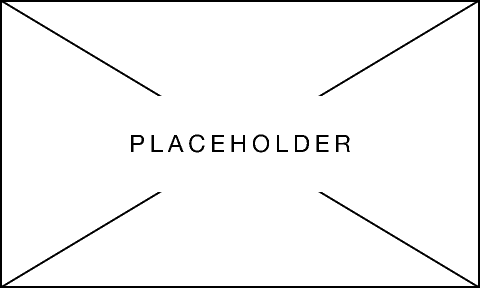
\includegraphics[width=5cm]{img/placeholder.png}
        \vspace{2cm}
        
        {\LARGE Some Placeholder Title \par}


        \vspace{1cm}
        \textbf{A Master Thesis}
        \vspace{0.5cm}
       
        written by
       
        \vspace{0.5cm}
        
        \begin{tabular}[t]{c@{\extracolsep{4em}}}
        \textbf{Name}\\
        my@email.dk\\
        potential-number \\
        \end{tabular}
        
        \vspace{8.0cm}
        
        \begin{center}
        The code for this project is available at\\
        \url{url-to-some-github}
        \end{center}
        
        \vfill
        
        \textbf{Overarching Institution}\\  
        Specific Department\\
        
        \vspace{0.5cm}
        
        Word Count : [some word count] \\
        Date of Hand In
        % \today
            
   \end{center}
\end{titlepage}

% preface
% \input{sections/0-preface}

% roman numbering for abstract, TOC, glossary etc.
\pagenumbering{roman}

% abstract
\clearpage
\begin{abstract}
\setlength{\parindent}{0pt}
\normalsize

% \noindent Some abstract text explaining the goal, methods and conclusion of the project. \\

% This project presents a new \gls{pnp} pipeline by excluding the vision systems and using purely tactile inputs to eliminate the weaknesses of vision algorithms such as transparency and reflectance. To develop this pipeline three subproblems were identified: tactile perception, pose estimation and in-hand manipulation. Tactile perception consisted of estimating the contact point, normals and skew forces. Using physics engine assistance, all three quantities were succesfully estimated. The pose estimation was successfully achieved on synthetic data with an orientation error less than \SI{5}{\degree} and translation error less than \SI{1}{\centi\meter} at \SI{10}{\percent} outliers. The in-hand manipulation problem was successfully solved using \gls{dapg}, which entailed an analysis of the training process and end performance. Finally, potential improvements to the pipeline is discussed for future iterations.

In this project, a novel pipeline for a \gls{pnp} task is presented, focusing on utilizing tactile inputs instead of vision systems to overcome the limitations of vision algorithms, such as transparency and reflectance issues. The development of this pipeline involved addressing three key subproblems: \gls{tp}, \gls{pe}, and in-hand manipulation. \gls{tp} involved accurately estimating the contact points, contact normals, and skew forces. The contact normals were successfully estimated using \gls{rls}, the contact points were found using the grasp matrix, while a \gls{dl} model was attempted to be used for skew force estimation without success. To compensate for the missing skew forces and cases of contact normals assistance of the Gazebo physics engine was applied successfully. The \gls{pe} task demonstrated promising results on synthetic data using \gls{gnc} for outlier rejection and \gls{rcqp} for transformation estimation. This resulted in an orientation error of \num{3} degrees and a translation error of  \SI{0.08}{\centi\meter} while in the presence of \SI{10}{\percent} outliers, which was within the criteria for success. For the in-hand manipulation problem, the use of \gls{dapg} proved successful in the MuJoCo dynamic simulator, and a comprehensive analysis of the training process and final performance was conducted. Lastly, potential enhancements for future iterations of the pipeline are discussed.



\end{abstract}

% table of contents
\clearpage
\tableofcontents

% workload distribution
\clearpage

\section*{Acknowledgements}

I would like to express my sincere gratitude to those who have supported and guided me throughout my thesis project. \medskip

First and foremost, I would like to extend my deepest appreciation to my thesis supervisor, Christoffer Sloth, Lector at SDU Robotics, for his exceptional guidance and support throughout the entire process. His expertise and knowledge in the field of robotics have been invaluable in shaping this project. \medskip

I would also like to thank Yitaek Kim for his invaluable support and sparring in solving key aspects of this project. His insights and advice have been critical to the successful completion of this thesis. \medskip

Furthermore, I would like to extend my thanks to Shadow Robotics for providing the underlying software for the project to build upon along with technical support, enabling this project. Their contribution has been essential in the successful completion of this project. \medskip

Finally, I would like to thank my family and friends for their unwavering support and encouragement throughout this journey. Their love and support have been a constant source of motivation and inspiration. \medskip

Once again, I express my deepest gratitude to all those who have played a significant role in this project.

\addcontentsline{toc}{section}{Acknowledgments}

% glossary & acronyms
\clearpage
\addcontentsline{toc}{section}{Acronyms and Terms}
\printglossary[type=acronym, title=Acronyms, style=mcolindex]
\printglossary[type=main, title=Terms]

% main document
\clearpage
\pagenumbering{arabic}
\glsresetall

% \pagebreak
% \chapter{Example section}\label{ch:example}

This document demonstrate the use of figures, references, SI units, glossary, math notation, lists, and otherwise relevant formatting specifications. Paragraphs are typically separated using \texttt{\textbackslash medskip}.\medskip

\begin{figure}[H]
    \centering
    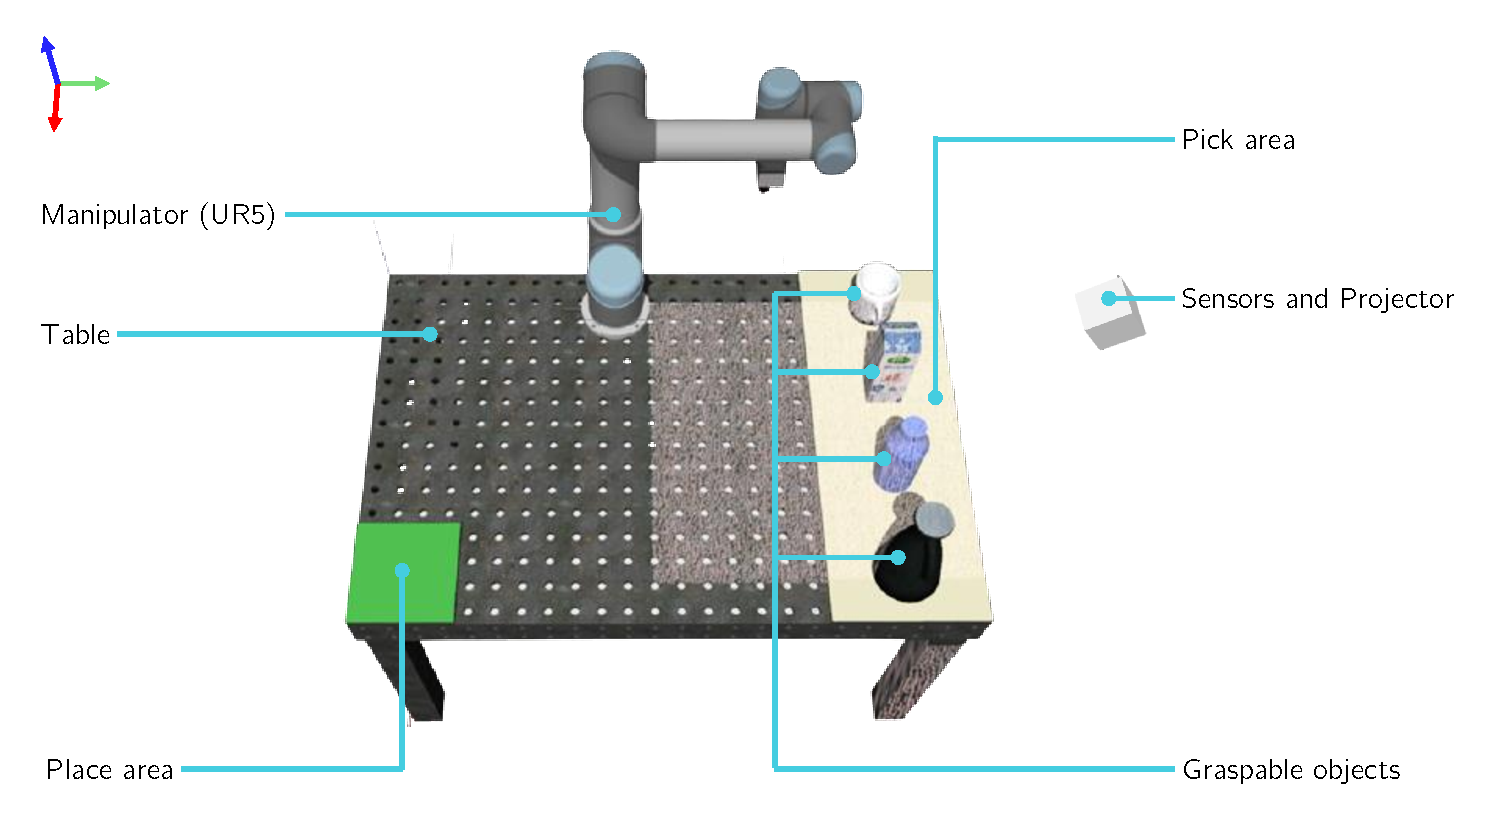
\includegraphics[width=.6\linewidth]{chapters/example/fig/figure.pdf}
    \caption{An example image using \acrlong{acronym-label}.}
    \label{fig:example-figure}
\end{figure}

To exemplify math notation, consider the mapping between the joint configuration of a robot
%
\begin{equation}
    \vec{q} = \rvec{q_1 & q_2 & \dots & q_n}\T,
    \label{eq:jnt-config}
\end{equation}

and \gls{glossary-label}, given as a homogeneous transformation
%
\begin{equation}
    \renewcommand{\arraystretch}{1.2}
    \tf{A}{B} = \begin{bmatrix}
        \tf[R]{A}{B}         & \tf[t]{A}{B} \\
        \vec{0}^{1 \times 3} & 1 
    \end{bmatrix},
\end{equation}

where \tf[R]{A}{B} and \tf[t]{A}{B} is the rotation and translation, respectively, from frame $\{A\}$ to frame $\{B\}$, denoted using a homogeneous transformation matrix $\mat{T}(\vec{q}) \in \mathbb{R}^{4 \times 4}$ as a function of the joint configuration in \eqref{eq:jnt-config}, as described in \cite{robotics-book}.\medskip

Complex table/figure hybrids with aligned captions and functioning labels can be implemented using \texttt{minipage}, as shown in \tabref{tab:example-table} and \figref{fig:example-plot}. Use \fakecite as a placeholder for citations.

\begin{center}
    \renewcommand{\arraystretch}{1.2}
    \begin{minipage}{.4\linewidth}
        \vspace{-10pt}
        \centering
        \begin{tabular}{|l|c|c|c|}
        \hline
        \diagbox[width=5.5em, font=\footnotesize\bfseries]{Method}{Pose} & 1 & 2 & 3 \\ \hline
        Linear    & \SI{18.97}{\second} & \SI{20.35}{\second} & \SI{22.85}{\second} \\ \hline
        Parabolic & \SI{13.66}{\second} & \SI{14.93}{\second} & \SI{17.33}{\second} \\ \hline
        \end{tabular}%
    \end{minipage}%
    \hfill%
    \begin{minipage}{.55\linewidth}
        \vspace{0pt}
        \centering
        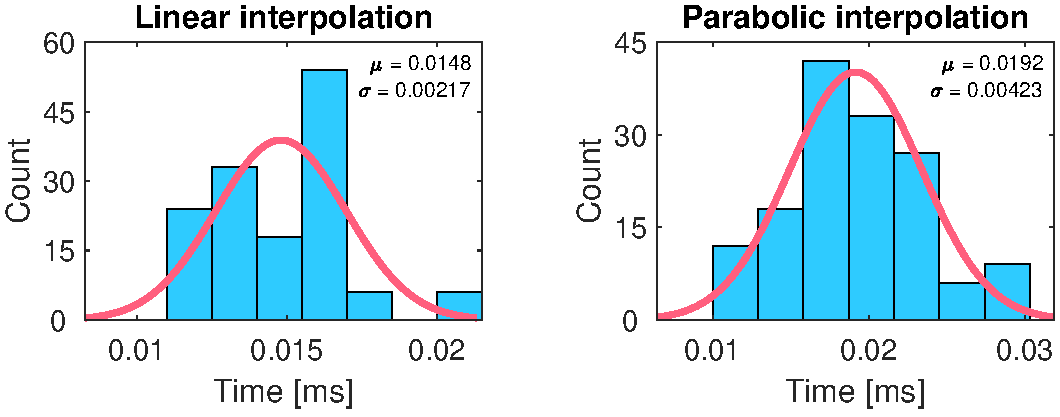
\includegraphics[width=.95\textwidth]{chapters/example/fig/plot.pdf}
    \end{minipage}%
    %    
    \vspace{15pt}
    %
    \begin{minipage}[t]{.4\linewidth}
        \vspace{0pt}
        \captionsetup{type=table}
        \captionof{table}{Trajectory durations of the interpolation-based trajectory generation methods.}
        \label{tab:example-table}
    \end{minipage}%
    \hfill%
    \begin{minipage}[t]{.55\linewidth}
        \vspace{0pt}
        \captionsetup{type=figure}
        \captionof{figure}{Average planning time for each of the interpolation-based trajectory generation methods.}
        \label{fig:example-plot}
    \end{minipage}%
\end{center}

For numbers, units and ranges, the \texttt{siunitx} package is used, which allows to express a number \num{10}, a range of \SIrange{5}{6}{\second}, or a SI unit of \SI{5.73 \pm 1.09}{\second}. Inline row-vectors (with the transpose symbol) can be written as $\vec{a} = \rvec{\vec{a}_p & \vec{a}_o}\T$, where as parentheses can be automatically written using $\qty(a, b)$ or $\qty{\frac{a}{b}, c}$. Also, shorthands for \mat{A}\inv, \mat{A}\pinv and \mat{A}\T.\medskip

\glsresetall

\pagebreak
\chapter{Introduction}\label{ch:intro}

\section{Context}\label{sec:intro-context}

% historical context
As of 2022 humanity has developed tools for unprecedented growth in wealth and technology on a global scale \fakecite. In such times a great deal of consumerism and interconnection is present with people needing product produced faster and more consistently than ever \fakecite. 
As one would expect, this creates a high demand for manufacturers to reliably and consistently being able to provide products, while also remaining flexible, as the demand for different product change rapidly. 
% argue for why automation is better
% https://www.fishmancorp.com/robotics-manufacturing/
% https://www.universal-robots.com/blog/solving-complex-problems-with-innovative-concepts-and-robotic-solutions/
In order to provide great volumes of products, manual labor has is essential as assembly, transport and manipulation processes rely on these. Due to these types of manual labor being largely done by unskilled workers, automation alternatives are being adopted which provides benefits. 
% this is referred to as industry 4.0
% benefits for employer
These include for the employer: Avoid having to pay monthly salaries to unskilled labored individuals doing manual tasks, here the automation solution only requires electrical energy and potential supervision by a qualified individual. Potential risks are also involved when hiring humans as the workforce can be inconsistent due to human error\fakecite or left out due to illness etc. Considerations with regards workers rights such as working conditions and wage also needs not to be considered. These cause production limitations in the form of stand still hours, such as bathroom and lunch breaks along with after work hours and holidays. 
% benefits for the employee 
This replacement of manual labor also benefits the employee, as boring and physically wearing work is automated, enabling the employees to take on different and less wearing roles. While the issue of labor unemployment becomes apparent solutions which provide support to already hired workers have been developed, such as \gls{cobot}\fakecite. \medskip

% categories of problems in robotics for factories
When implementing automation of production lines using robotics, certain categories of problems are revealed. These include: Assembly, alteration and \gls{pnp}, the last being the one of interest in this project. 
\section{Problem Description}\label{sec:intro-problem-description}
% applications
Pick and place \gls{manipulator}s are used in a wide variety of different fields such as 
sorting of waste \cite*{robotic-pick-and-toss-facilitates-urban-waste-sorting}
handling of food \cite*{automation-of-mobile-pick-and-place-robotic-system-for-small-food-industry}\cite*{development-of-a-food-handling-soft-robot-hand-considering-a-high-speed-pick-and-place-task} and factory bin picking \cite*{real-time-industrial-bin-picking-with-a-hybrid-deep-learning-engineering-approach} \cite*{a-bin-picking-benchmark-for-systematic-evaluation-of-robotic-pick-and-place-systems} \cite{generic-development-of-bin-pick-and-place-system-based-on-robot-operating-system}. The solutions in these industries are examples of subcategories under the pick and place problem, namely sorting and bin picking. Since both of these are sub categories of the pick and place problem, they fundamentally follow the same sequential four phases from start to end. 
% All of these problems fundamentally contain the same structure as shared among all pick-and-place problems.
These steps being pre-grasping, grasping, transport, and placement \cite*{a-bin-picking-benchmark-for-systematic-evaluation-of-robotic-pick-and-place-systems} for traditional .
% pre-grasp
The pre-grasp phase involves localizing the object(s), potentially estimating their pose and executing the trajectory to move the end effectors grasp, collision free to said object(s). Here different potential grasp can be considered in order to determine the best pose for the end effector.
% grasping
In the grasping phase the end effector gasps the object in such a manner that the object's entire weight is supported by the \gls{ee}, and ends when the object no longer is in contact with the environment, which often is the container holding the object.
% transport
The transportation phase involves the motion of the manipulator to move from the pose achieved after the grasping phase, to a pose ready for placement of the object in the desired placing area or fixture. Here considerations may be needed with regards to how much force and torque the \gls{ee} can tolerate without losing the object.
% placement
Finally the goal of the placing phase is to place the object within the placing area or fixture in a desired end pose. Here the constraints on the end pose might differ significantly based on the application, as the pose of greens in a crate might need less precision than if the manipulator hands a bolt to the next robotics system in the pipeline. \medskip

While these phases make up a traditional \gls{pnp} systems, certain assumptions are made regarding the objects of interest in order for this pipeline to function. Specifically the localization and pose estimation of the pre-grasp phase are assumed possible due to \gls{cv} often being the sensory system for such tasks. Due to \gls{cv} techniques mimicking the human eye the field's maturity has generated a wide range solution proposals to these problems.


solutions to computer vision: classical,old fashion, deep learning based 

deep learning on transparent objects and reflective objects, shown less than ideal results

classical approaches% https://ieeexplore.ieee.org/abstract/document/7860048


vision has been used for many years \fakecite 


% traditional pipeline makes assumptions -> 

% ind end effector pose est
\section{Thesis Overview}\label{sec:intro-thesis-overview}































































% The developments in robotics as a field has over the past years provided automation solutions to execute repetitive manual tasks with high efficiency and reliability \fakecite. One of the most common tasks being pick and place tasks which involves picking un an object from one position and placing is in another. This is can be parted into the following subparts: Object localization, pose estimation, grasping and placing. In the solutions currently present for industrial use \gls{cv} is used for object localization and \gls{pe} due to the low cost of cameras and the fields maturity. However, while these solutions may be sufficient for certain tasks they fundamentally suffer from the weaknesses introduced by vision techniques. These include a great number of outliers caused by occlusions, reflecting, transparent or homogeneous surfaces, and repetitive structures when solving the \gls{corr-problem}. These problems as of the writing of this project have jet to be completely solved. Promising results have been found with the rise of \gls{dl} which in present time has proven its versatility and provides proof of concept solutions for narrow cases in pose estimation of transparent \cite{6dof-pose-estimation-of-transparent-object-from-a-single-rgb-d-image} and reflective \medskip

% \begin{minipage}{0.45\textwidth}
% 	objects \cite{6d-pose-estimation-of-objects:-recent-technologies-and-challenges}. This is relevant since industrial settings often contain transparent and especially reflecting objects as metallic parts tend to appear frequently and have high reflectances. To solve these problems this project aims to perform in-hand pose estimation through only the use of tactile sensors. Specifically this will be done on a Shadow Dexterous Hand \cite{shadow-dex-hand} with 20 \gls{dof}. Using tactile inputs rather than visual, eliminates the weaknesses mentioned above. A schematic showing the hand can be seen in \figref{fig:shadow-dex-hand-schematic}. Using this approach, the overall problem can be partitioned into 3 sub-problems labeled problem 1, 2 and 3. Problem 1 involves modeling the contact between the gripper's fingers and the object, also referred to as tactile perception. Problem 2 is to convert the collected data from problem 1 to meaningful surface data, treat these data as features and use them to estimate pose candidates. Finally problem 3 involves in-hand manipulation, such that further information is gained by probing the object. Here new desired surface points are found through intelligent probing such that strong surface features are found to better identify the object's correct pose. \medskip
% 	\end{minipage} 
% 	\hfill
% 	\begin{minipage}{0.45\textwidth}
% 	\begin{figure}[H]
% 		\begin{small}
% 			\begin{center}
% 				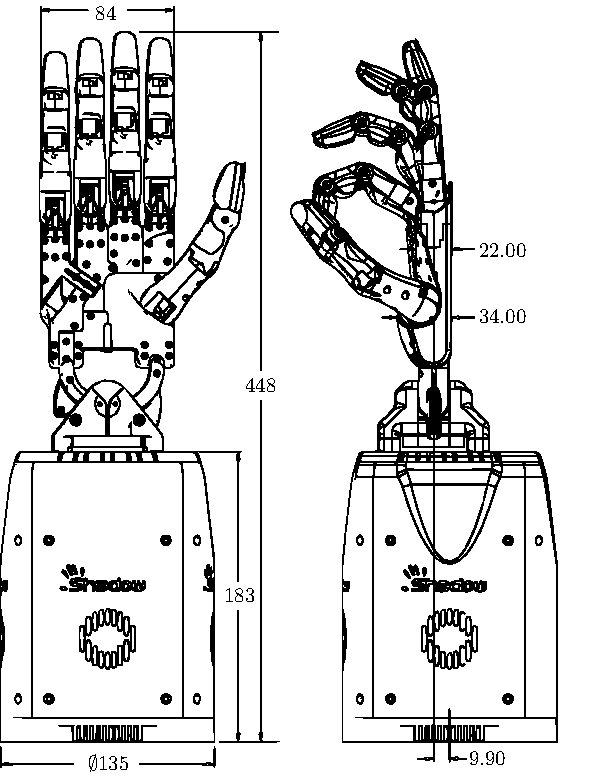
\includegraphics[width=0.95\textwidth]{chapters/introduction/fig/shadow-dex-hand-vector.pdf}
% 			\end{center}
% 			\caption{Schematic of Shadow Dexterous Hand from Shadow Robots, based on \cite{shadow-dex-hand-schematic}. The measurements are in \SI{}{\milli\metre}.}
% 			\label{fig:shadow-dex-hand-schematic}
% 		\end{small}
% 	\end{figure}
% \end{minipage}

% Thus the hypothesis of this projects $\text{H}_1$, will be testing if intelligent probing for strong features increases in-hand pose estimation performance, with the null hypothesis $\text{H}_0$ being that there is no statistical significant difference in the pose estimation performance of the system if the probing is done randomly or intelligently at a certainty level of \highlight{95\%}. Here pose estimation performance is quantified in terms of mean execution time for estimating the pose with an accuracy greater than \highlight{95\%}. \medskip

% The development of this project is done in the \gls{docker} provided by Shadow Robotics for simulation, control and development of the hand \cite{shadow-dex-github}. Here a hardware-simulation agnostic \gls{ros} \cite{ros} control \cite{ros-control} interface is found, which contains fundamental tools to interact with the robot hand. The dynamic simulation environment Gazebo \cite{gazebo} is likewise packaged as part of the \gls{docker} and is thus the one used for this project.
% To solve the problems presented, the \gls{ros} packages in \tabref{tab:software-package-table} will be applied, where \texttt{ros\_utils} and \texttt{in\_hand\_pose\_estimation} will be developed during this project.

% \begin{table}[h]
% 	\begin{small}
% 		\begin{center}
% 			\begin{tabular}[c]{ | l r | l | } \hline
% 				\cellcolor{tableheader} \textbf{Package}           & \cellcolor{tableheader} & \multicolumn{1}{l|}{\cellcolor{tableheader} \textbf{Description}} \\ \hline \hline
% 				\texttt{in\_hand\_pose\_estimation}                & \meta{meta} & \textbf{Project package of the in-hand pose estimation system} \\ \hline
% 				\hspace{0.3cm} \texttt{in\_hand\_pose\_estimation} &             & Integration of the full in-hand pose estimation pipeline  \\ \hline
% 				\hspace{0.3cm} \texttt{sr\_tactile\_image}         & \pkg{pkg}   & Extraction of tactile perception  \\ \hline
% 				\hspace{0.3cm} \texttt{sr\_pose\_estiamtion}       & \pkg{pkg}   & Estimate the pose of object based on tactile perception \\ \hline
% 				\hspace{0.3cm} \texttt{sr\_hand\_manipulation}     & \pkg{pkg}   & Manipulate object in hand to probe for strong features \\ \hline \hline
% 				\texttt{sr\_common}                                & \meta{meta} & \textbf{Shadow package for commonly used tools} \\ \hline
% 				\hspace{0.3cm} \texttt{sr\_common}                 &             & Implements commonly used tools such as messages \\ \hline
% 				\hspace{0.3cm} \texttt{sr\_robot\_msgs}            & \pkg{pkg}   & Messages used to communicate with the robot hand  \\ \hline 
% 				\hspace{0.3cm} \texttt{\dots}                      &             &  \\ \hline \hline
% 				\texttt{sr\_core}                                  & \meta{meta} & \textbf{Shadow package for core tools} \\ \hline
% 				\hspace{0.3cm} \texttt{sr\_core}                   &             & Implements core features of the hand such as hardware interfacing \\ \hline
% 				\hspace{0.3cm} \texttt{sr\_hand}                   & \pkg{pkg}   & Contains the hand commander for controlling the robot hand  \\ \hline
% 				\hspace{0.3cm} \texttt{\dots}                      &             &  \\ \hline \hline
% 				\texttt{ros\_utils}                                & \pkg{pkg}   & \textbf{Utilities for interfacing ROS/Gazebo/MoveIt/Eigen etc} \\ \hline
% 			\end{tabular}
% 		\end{center}
% 		\caption{Software packages used in the in-hand pose estimation system.}
% 		\label{tab:software-package-table}
% 	\end{small}
% \end{table}

% To present this work, the \gls{sota} solutions to each of the three problems described above will be presented in \chapref{ch:state-of-the-art}, where the best fitting methods for this use case will be chosen. In \chapref{ch:1-tactile-perception} to \chapref{ch:3-in-hand-manipulation} these solutions will be presented, analyzed, and their performance discussed and concluded upon. In \chapref{ch:4-system-integration} the system integration will be presented and the total performance of the system will be concluded. Finally in \chapref{ch:discussion} and \chapref{ch:conclusion} the results and methods will be discussed with potential improvement for future iterations and the project til be concluded.

\pagebreak

\chapter{State of the Art} \label{ch:state-of-the-art}

\section{Problem 1 - Tactile Perception} \label{sec:lit-rev-problem-1}

In order to model the contact between the \gls{ee}'s tactile sensors, eight different taxonomies are present\cite*{articulated-hands-force-control-and-kinematic-issues} whereas three most common ones are \gls{pwof}, \gls{hf} and the \gls{sf} model as shown in \figref{fig:contact-models}, within the field of robotics\cite[Chapter 37]{handbook-of-robotics}. \medskip

\begin{figure}[h]
	\centering
	\begin{subfigure}[b]{0.3\textwidth}
		\centering
		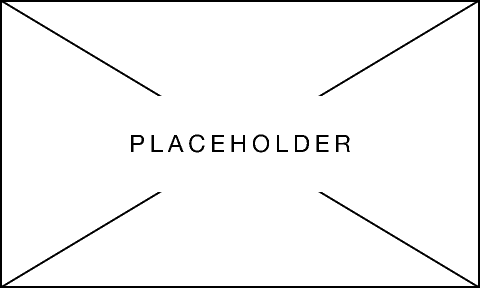
\includegraphics[width=\textwidth]{img/placeholder.png}
		\caption{Point contact model without friction.}
		\label{fig:pwof}
	\end{subfigure}
	\hfill
	\begin{subfigure}[b]{0.3\textwidth}
		\centering
		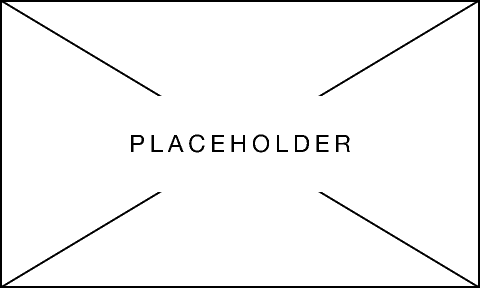
\includegraphics[width=\textwidth]{img/placeholder.png}
		\caption{Point contact model with friction.}
		\label{fig:hf}
	\end{subfigure}
	\hfill
	\begin{subfigure}[b]{0.3\textwidth}
		\centering
		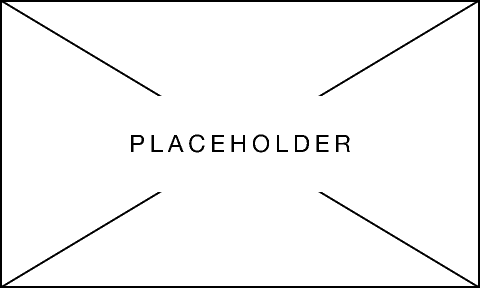
\includegraphics[width=\textwidth]{img/placeholder.png}
		\caption{Soft-finger model.}
		\label{fig:sf}
	\end{subfigure}
	   \caption{The three most commonly used contact models.}
	   \label{fig:contact-models}
\end{figure}

% no friction
The \gls{pwof} model, as shown in \figref{fig:pwof}, can only represent forces along with the normal of the object's surface at the point of contact and thus the model does not support surface deformations between the two contacting objects. This model is applied in cases where very little deformation is present along with the contact being slippery\cite[Chapter 38]{handbook-of-robotics}.\medskip

% Hard finger
The \gls{hf} model, as shown in \figref{fig:hf}, is representative when the friction between objects is great enough to be significant, while the contact deformation is small enough to ignore friction moments\cite[Chapter 38]{handbook-of-robotics}. To model the friction acting on the contact point a great number of methods exist, the most common being the Column friction with different modifications depending on the use case\fakecite. \medskip

% Soft finger
The \gls{sf} model, as shown in \figref{fig:sf}, is used to represent scenarios where both friction and surface deformations are great enough to be impactful in the systems behavior. Due to deformations of the finger an additional torsional moment about the contact normal will be present.
\cite[Chapter 38]{handbook-of-robotics}  \medskip


% draw the model as applied in our case

% subcategories of sf models
Based on the contact model categories described above, the most representative is \gls{sf} since these models can provide descriptions of the contact surface topology, and thus enable the solving of the \gls{iep} by deriving surface features for pose estimation. Within the category of \gls{sf} models a method fit for this project's use case is to be chosen to solve problem \ref{prob:1}. \gls{sf} models can furthermore be divided up into three different categories: \gls{aebm}, \gls{efm} and \gls{fem} \cite{a-modified-elastic-foundation-contact-model-for-application-in-3d-models-of-the-prosthetic-knee}. \medskip


% reformulate
% \gls{aebm} are theoretical formulations of elasticity calculating contact areas and stresses on both the surface and the sub-surface of the contacting bodies, but are restricted to simple geometries. The classical Hertz contact model (Hertz, 1882; Johnson, 1995)

% 

% 1) I want to model contacts
% 2) there exist 8 different modeling taxonolies
% 3) three are most common
% 	3.a) explain each of the three 
% 4) since soft supports the behavior we want we choose that one
% 5) what method categories exist within soft finger modelling



% In order to model the pressure distribution in the contact area different models have been devel-
% oped that fall into three main categories: analytical elasticity-based models, elastic foundation models
% (EFM) and finite element models (FEM) (Pérez-González et al., 2008). Analytical models are based on
% theoretical formulations of elasticity calculating contact areas and stresses on both the surface and the
% sub-surface of the contacting bodies, but are restricted to simple geometries. The classical Hertz con-
% tact model (Hertz, 1882; Johnson, 1995) and others derived from it are part of this category. However,
% robotic fingertips are made of nonlinear elastic materials. For that reason, the Hertzian contact model
% does not accurately represent this type of contact. EFMs were developed in order to allow a simple
% discrete contact calculation in more general surface geometries modelling the deformable part of the
% contact as a layer over a rigid base, and a series of discrete and independent springs in the contact
% normal direction. An application of this category of models is presented in Section 3.4 where it is used
% to create a simulation of a general tactile sensor and validated in robot grasping applications. FEMs
% have been increasingly used over recent years given that they supply information about the sub-surface
% stresses and strain in volumetric finite elements. However, they are excessively time consuming for fast
% simulation in dynamic grasping and manipulation models. Therefore, simplified numerical models are
% interesting alternatives.

% with friction



% soft finger


% When choosing a representative contact model, two overarching groups exist: linear and non linear models. While the linear models often are too simple to properly represent the real phenomena, their simplicity often make them a popular choice for practical reasons. \medskip

% Within the linear models group we find the most common model: The Hertzian contact model\cite*{on-the-contact-of-rigid-elastic-solids-and-on-hardness}. This model makes the assumptions that
% the objects consist of linear elastic materials when in contact and the contact deformations are small compared to the dimension of object.


% non-linear models

% When considering the non linear contact models, the simpler 

% The Hertzian contact model specifically assumed linear elastic objects in contact with small deformation. Later, the study of contact mechanics became a branch in mechanics. One of the important results in his seminal paper postulated that where N is the normal force, a is the radius of circular contact area, and C is a proportional constant. Equation (2), derived by Hertz [13], describes the growth of radius of circular contact area as proportional to the normal force raised to the power of 3 1 . It is important to note that Hertz had assumed that ( i ) the contact is linear elastic and ( ii ) the deformation is small.



% 

% \begin{center}
%     \renewcommand{\arraystretch}{1.2}
%     \begin{minipage}{.48\linewidth}
%         \vspace{0pt}
%         \centering
%         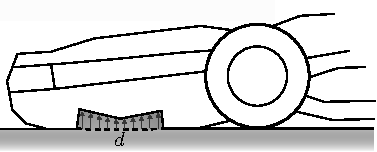
\includegraphics[width=.95\textwidth]{chapters/modeling/fig/measure-displacement.pdf}
%     \end{minipage}%
%     \vspace{15pt}
%     \begin{minipage}[t]{.48\linewidth}
%         \vspace{0pt}
%         \captionsetup{type=figure}
%         \captionof{figure}{The friction forces $\mathbf{f}_f$ and contact model keeps the object $\{O\}$ from slipping between the \gls{ee}'s fingers when the gravitational pull $\mathbf{f}_g$ is acting on it.}
%         \label{fig:measure-displacement}
%     \end{minipage}%
% \end{center}

% in order to perform tactile perception we need to model the contact between the end effector and the object of interest -> 
% 	This model needs to provide descriptions of parameters such as pressure and area for the contact to be 
% 	This model needs to contain the pressure and deformation caused by the contact in order to recreate the surface of contact





% What are contact models and what do they describe?
% For tactile perception it is needed to model the contact between the robotic manipulator finger and the object. The model will here 

% we need a model


%  what do we wish to model contact forces and how they can relate to deformation. Friction to determine how much force to apply in order to keep the object in the grasp.


%  


% flush out what exactly the model i want to use looks like


% When considering different methods for modeling contact interfaces, each can be categorized depending on which parameters the model describe the relation between. This results in the following groupings: contact-area-force models, stress-strain models, force-displacement models and 

% How are models grouped and what groupings exist?

% Contact models can be grouped based on the what parameters the relation is describing.







% Contact Area vs. Applied Force


% Hertzian contact model

% Soft Contact Model (More general Hertzian model)

% Viscoelastic Soft Contact Model.

% 	 Kelvin–Voigt/Maxwell model
% 	  Fung’s model

% Other contact models (research)



% Boussinesq–Cerruti’s

% Love’s solution 




% Love's formulation 




% What is tactile perception? Why is it relevant? \\
% How is a tactile sensor constructed \cite{recent-progress-in-technologies-for-tactile-sensors}
% what different types exist and which one is present in the model provided.


% \textit{"Representations of tactile data are commonly either inspired by machine vision feature descriptors"}

% often used in computer vision context, where each tactile image 

% Addressing the problem 





\section{Problem 2 - Pose Estimation} \label{sec:lit-rev-problem-2}

\section{Problem 3 - In-Hand Manipulation} \label{sec:lit-rev-problem-3}

\pagebreak
\chapter{Tactile Perception} \label{ch:1-tactile-perception}

\section{Introduction} \label{sec:1-tactile-perception-introduction}

\begin{itemize}
	\item start with performance specifications regarding the two problems the tactile perception should be able to solve: can the are the points representative, according to the source yes, but are the normals also representative. This is important for the pose estimation problem. When manipulating the object the finger needs to be able to exert enough friction to be able to hold the object, is this true. compute the contact friction and see if it is stronger than the gravity on the subject. Use numbers to verify if the performance is acceptable
	\item 
\end{itemize}


\section{Method}\label{sec:1-tactile-perception-method}


\section{Experimental Setup}\label{sec:1-tactile-perception-experimental-setup}


\section{Results}\label{sec:1-tactile-perception-results}


\section{Discussion \& Conclusion}\label{sec:1-tactile-perception-discussion-and-conclusion}



% \section{Related Work} \label{sec:1-tactile-perception-related-work}

% Here we cite the related work by \texttt{\textbackslash cite\{source-label\}} like this \cite{recent-progress-in-technologies-for-tactile-sensors}

\pagebreak
\chapter{Pose Estimation}\label{ch:2-pose-estimation}

This chapter focuses on pose estimation, specifically addressing the optimization-based PCR problem. It introduces the \gls{rcqp} and \gls{gnc} methods used to solve this problem and evaluates their performance in estimating the pose of the object of interest. The primary objective is to assess the extent to which \gls{rcqp} and \gls{gnc} can accurately estimate the position and orientation of the object, aiming for an orientational error less than \SI{5}{\degree} and a positional error less than \SI{1}{cm} as mentioned in \secref{sec:intro-problem-description}. Importantly, it is assumed throughout the chapter that the object of interest is known, eliminating the need for classification.\medskip

To achieve this goal, the chapter presents the methodologies employed, the experimental setup, and the obtained results. The results obtained in this chapter encompass two main aspects 1) synthetic source data is utilized, and generated from the target data to ensure accurate correspondences. This allows for the evaluation of the methods' robustness by introducing varying percentages of outliers. 2) the methods are applied to sampled data from~\chapref{ch:1-tactile-perception} to estimate the pose of the object based on computed correspondences.\medskip

Furthermore, in addition to solving the pose estimation problem, the chapter includes an estimation of the signal-to-outlier ratio. This is achieved by utilizing the weights produced by \gls{gnc}. The estimation is conducted firstly on the synthetic source data where the ground truth is known and secondly on the sampled source data where the outlier ratio is unknown.

% In this chapter, the pose estimation is presented as an optimization-based \gls{pcr} problem, along with the \gls{rcqp} and \gls{gnc} methods used for solving said problem and their performance in solving the \gls{pcr} problem. The goal of this chapter is to determine to what extent \gls{rcqp} and \gls{gnc} are capable of sufficiently estimating the pose of the object of interest. According to~\ref*{sec:intro-problem-description} \SI{95}{\percent} accuracy in both position and orientation estimates. It is throughout this chapter assumed that the object of interest is known, and thus no classification is needed. \medskip

% This is achieved by presenting the methods used, along with the experimental setup and results. The results gained in this chapter will be two fold 1) The methods will be performed on synthetic source data, meaning point clouds generated from the target data to ensure accurate correspondences while enabling the enforcement of certain outliers percentages, which will be applied to determine the methods robustness. 2) the methods will be applied on sampled data from~\chapref{ch:1-tactile-perception} to determine the object's pose from computed correspondences. \medskip

% In addition to the pose estimation problem solved, the signal-to-outlier ratio is estimated based on the weights produced by \gls{gnc}, first on the synthetic source data where the \gls{gt} in known and secondly on the sampled source data where the outlier ratio is unknown. \medskip

\section{Problem}\label{sec:2-pose-estimation-problem}



In this chapter, the \gls{rcqp} method with \gls{gnc} will be presented along with its performance in solving the \gls{pcr} problem. The produced source data \mat{X} in~\chapref{ch:1-tactile-perception} is a \gls{pc} of the form
%
\begin{equation} \label{eq:data-matrix-structure}
	\mat{X} = 
	\begin{bmatrix}
		c_x & c_y & c_z & n_x & n_y & n_z \\
		c_x & c_y & c_z & n_x & n_y & n_z \\
		 &  & \vdots &  &  &  \\
		c_x & c_y & c_z & n_x & n_y & n_z \\
	\end{bmatrix}\inR{M\times 6},
\end{equation}

where \mvar{\vec{c}=\rvec{c_x, c_y, c_z}} is a contact point, \mvar{\vec{n}=\rvec{n_x, n_y, n_z}} is the corresponding point's normal vector and \mvar{M} is the number of source data points. The target data \mat{Y} is structured likewise, except for the number of target data points being \mvar{N}, where \mvar{N\ge M}. For convenience, the \mvar{i}'th row in source data is referred to as \mvar{\vec{x}_i} while the \mvar{i}'th row in the target data is referred to as \mvar{\vec{y}_i}. \medskip 

Under the assumption of already knowing the object of interest, \mat{Y} is generated from the mesh of the Stanford bunny model~\cite{stanford-bunny} with a resolution of \num{10,000} data points as shown in figure~\figref{fig:pe-pc-target}. The source data \mat{X} can likewise be seen in~\figref{fig:pe-pc-source} as generated in~\chapref{ch:1-tactile-perception}. \medskip

\begin{figure}[!h]
	\centering
	\begin{subfigure}[b]{0.48\textwidth}
		\centering
		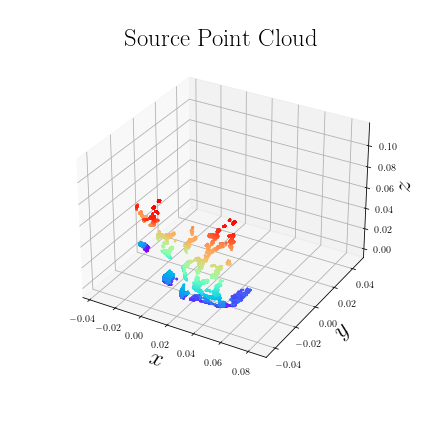
\includegraphics[width=\textwidth]{chapters/1-tactile-perception/fig/matplotlib/pc_source.png}
		\caption{The source data \mat{X} \gls{pc} generated from simulated contact points, normals are also included, but not illustrated here for the sake of simplicity.}
		\label{fig:pe-pc-source}
	\end{subfigure}
	\hfill
	\begin{subfigure}[b]{0.48\textwidth}
		\centering
		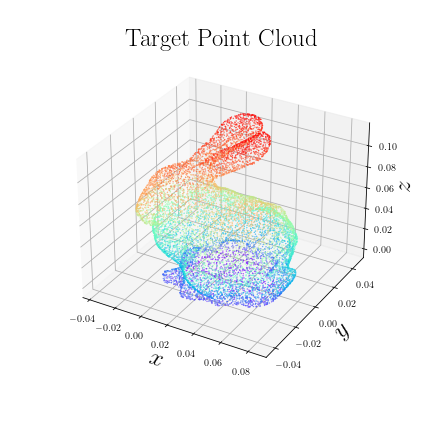
\includegraphics[width=\textwidth]{chapters/1-tactile-perception/fig/matplotlib/pc_target.png}
		\caption{The target \gls{pc} generated by sampling the model mesh with \num{10,000} points, normals are also included, but not illustrated here for the sake of simplicity.}
		\label{fig:pe-pc-target}
	\end{subfigure}
	\caption{3D plots showing source and target data.}
	\label{fig:pe-contact-position-gazebo}
\end{figure}

To determine the transformation between the two point clouds \tf[T]{\mat{X}}{\mat{Y}}, correspondences must be found according to the \gls{corr-problem}. Due to \mat{X} being produced by local sensing with high-density sensor regions, a \gls{pc} feature which exploits this is desired. The one chosen is \gls{fpfh} which is a feature descriptor used in 3D point cloud analysis and registration tasks and provides a feature matrix \mvar{\mat{F}\inR{N\times 33}}. The feature descriptor calculates a histogram representation for each point by considering the local geometric properties of its neighboring points. It captures information about the distribution of surface normals and distances between points within a local neighborhood. Additionally, \gls{fpfh} is computationally efficient and provides robust feature representations. \medskip

Using the correspondences found from \gls{fpfh}, the pose estimation problem can be formulated as an optimization problem for determining the optimal homogeneous transformation matrix between the two points clouds \tf[T]{\star\mat{X}}{\;\;\mat{Y}}, which for convenience is from now on referred to as \tf[T]{\star}{}, by
% \colorbox{red}{obs, what makes GNC special is the fact that it changes the \mvar{\mu} either up or down depending on GM or TLS, which gradually causes non-convexity. RCQP is used to solve for x in gnc paper}
%
\begin{equation} \label{eq:point-cloud-registration-problem}
	\tf[T]{\star}{} = \arg \min_{(\mat{R},\vec{t})\in\SE (3)} \sum^M_{i=1} d_{P_i}\left( \vec{x}_i, \mat{T} \right)^{2}.
\end{equation}

Here \mvar{\tf[T]{}{}=(\tf[R]{}{}, \vec{t})\in\SE (3)} refers to the homogeneous transformation matrix \mvar{\tf[T]{}{}\inR{4\times 4}} from \mat{X} to \mat{Y}, which consists of a rotation matrix \mvar{\tf[R]{}{}\inR{3\times 3}} and a translation vector \mvar{\vec{t}\inR{3}} as members of the \gls{se} group in 3D, and \mvar{d_{P_i}(\cdot)} is the distance to the matching primitive \mvar{P_i}. The primitives of interest in this project are point-to-point and point-to-plane, due to the presence of contact normals. The distance function will differ between primitive, and thus the ones of interest are listed as
%
\begin{align}\label{eq:distance-functions}
	\min_{\vec{y}'\in P} \|\vec{x}-\vec{y}'\|^2_2 &=  \\
		& =\|\vec{x}-\vec{y}\|_2^2=\|\vec{x} - \vec{y}\|_{\mat{I}_3}^2 & \text{(point)} \\
		& = \left( \vec{n}^\T (\vec{x} - \vec{y}) \right)^2=\|\vec{x}-\vec{y}\|^2_{\vec{n}\vec{n}^\T} & \text{(plane)}
\end{align}
where \mvar{\vec{y}'\inR{3}} is the term used as a substitute for each primitive, \vec{x} is a 3D point, \mvar{\mat{I}_3\inR{3\times 3}} is the identity matrix and \mvar{\vec{n}_i} is the unit normal vector for a plane. However, these are highly sensitive to outliers and noise, and thus a robust cost function \mvar{\rho(\cdot)} is applied. Of the two presented in~\cite{graduated-non-convexity-for-robust-spatial-perception:-from-non-minimal-solvers-to-global-outlier-rejection} i.e. \gls{tls} and \gls{gm}, \gls{tls} was chosen, as it shows slightly better performance. The problem can thus be written as
%
\begin{equation}\label{eq:point-cloud-registration-problem-robust}
		\tf[T]{\star}{} = \arg \min_{(\mat{R},\vec{t})\in\SE (3)} \sum^M_{i=1} \rho\left(d_{P_i}\left( \vec{x}_i, \mat{T} \right)^{2}\right).
\end{equation}

However solving the \gls{pcr} problem globally is still a challenging endeavor, even when known correspondences are available, primarily because of the non-convex nature of the rotation constraints, where \mvar{\mat{R}\in\SE (3)}. For this reason, global approaches are applied to deal with the problem of local minima, by starting from a convex problem, and gradually increasing the non-convexity until the original problem is retrieved, this being the purpose of \gls{gnc}. However, not all solutions when found globally are of interest, as the structure of the rotation matrix places certain quadratic constraints on the solution to be valid, such as orthonormality. From a then estimated optimal \mvar{\mat{R}^\star}, the optimal translation \mvar{\vec{t}^\star} can be found~\cite{convex-global-3d-registration-with-lagrangian-duality}. Thus the problem has been reduced to an orientation estimation problem to find \tf[R]{\star}{}.

\section{Method}\label{sec:2-pose-estimation-method}

% The method chosen for this chapter is twofold: first outliers are rejected using \gls{gnc} and \gls{rcqp} for determining the optimal transformation \mvar{\mat{T}^\star}. One of the common problems of \gls{pcr} is the presence of outliers, exceeding \SI{95}{\percent} is not uncommon~\cite{guaranteed-outlier-removal-for-point-cloud-registration-with-correspondences}. Outlier removal is thus necessary, which is chosen in the form \gls{gnc}. To find correspondences, a point cloud feature which utilizes the clusters of points produced by the fingertips. Thus the \gls{fpfh} descriptor is chosen. Using these features descriptors \mvar{d_{t}} are found for the target data i.e. \mat{Y} and the source data \mat{X} i.e. \mvar{d_s}. Using these matching pairs of points are found using an exhaustive search and a similarity threshold of \num{0.01}

% the distance is the normalized Euclidean distance between the matching features.

% The data is then organized in matrices \mat{X} and \mat{Y} for the source and target data, but organized such that each row corresponds 

% in the outlier-free case, we can simply solve

% \begin{equation} \label{eq:outlier-free-problem}
% 	\tf[T]{\star}{} = \arg \min_{\mat{T}\in\SE (3)} \sum^M_{i=1} r^2\left( \vec{x}_i, \tf[T]{}{} \right),
% \end{equation}

% where \mvar{\vec{x}_i} is the \mvar{i}'th sample in the data matrix \mat{X}, \mvar{\tf[T]{}{}\inR{4\times 4}} is a homogeneous transformation matrix and \mvar{\tf[T]{\star}{}\inR{4\times 4}} is the 

% quadratic cost in the least squares problem (1) with a robust cost $\rho(\cdot)$:


\subsection{Graduated Non-Convexity}\label{subs:2-pose-estimation-graduated-non-convexity}

Rather than applying \gls{gnc} for optimizing the robust cost function \mvar{\rho(\cdot)}, we fix constant \mvar{\mu} to instead optimize
%
\begin{equation}
	\tf[R]{\star}{}=\arg \min_{\mat{R}\in\SE (3)} \sum^M_{i=1} \rho_\mu \left(d_{P_i}\left(\vec{x}_i, \mat{R} \right)^{2}\right)
\end{equation}
However, since this problem cannot be solved using a non-minimal solver, the \gls{br} duality can be applied, given the necessary conditions are met. These conditions are as follows
%
\begin{align}\label{eq:br-condition-1-2-3}
	\lim_{z\rightarrow 0} \phi'(z) &= 1 & \text{condition 1} \\
	\lim_{z\rightarrow \infty}\phi'(z) &= 0 & \text{condition 2} \\
	\phi''(z) &< 0 & \text{condition 3}
\end{align}
Here \mvar{\phi(z)} is defined with respect to the robust cost function \mvar{\rho} in the following manner
%
\begin{equation}
	\phi(z) \overset{\cdot}{=} \rho(\sqrt{z}).
\end{equation}

Condition 1 indicates that as the argument \mvar{z} approaches \num{0}, the derivative of \mvar{\phi(z)} approaches \num{1}. Geometrically, it implies that near the origin, the function \mvar{\phi(z)} grows at a similar rate as the square root function itself. This behavior ensures that small values of \mvar{z} are penalized appropriately by the robust cost function \mvar{\rho(\cdot)}, allowing for robustness against outliers or deviations from the assumed distribution. \medskip

Condition 2 states that as \mvar{z} approaches \mvar{\infty}, the derivative of \mvar{\phi(z)} tends towards \num{0}. This implies that as the argument becomes larger, the function \mvar{\phi(z)} approaches a plateau or a constant value. Consequently, large values of \mvar{z} have a diminishing effect on the robust cost function, making it less sensitive to extreme observations. \medskip

Condition 3 states that the second derivative of \mvar{\phi(z)} is negative, indicating that the function \mvar{\phi(z)} is concave. This concavity is crucial as it ensures that the robust cost function \mvar{\rho(\cdot)} is monotonically increasing. In other words, as the argument \mvar{z} increases, the robust cost increases as well. This property is desirable in robust estimation problems, as it helps in downplaying the impact of outliers or influential points on the overall estimation. \medskip

All of these conditions are met by the \gls{tls}~\cite{graduated-non-convexity-for-robust-spatial-perception:-from-non-minimal-solvers-to-global-outlier-rejection}.\medskip

With these conditions fulfilled, the \gls{br} duality enables
%
\begin{equation}\label{eq:br-result}
	\arg \min_{\mat{R}\in\SE (3)} \sum^M_{i=1} \rho_\mu \left(d_{P_i}\left( \vec{x}_i,\mat{R} \right)^{2}\right) = 
	\arg \min_{\substack{\mat{R}\in\SE (3),\\ w_i\in [0,1]}} \sum^M_{i=1} \left[ w_i d_{P_i}\left( \vec{x}_i,\mat{R} \right)^{2} + \Phi_{\rho_\mu}(w_i)\right],
\end{equation}
whereas the rightmost side will be the problem of interest. In this expression \mvar{w_i\in[0,1]\forall i=1,2,\dots,N} are weights associated with each measurement \mvar{\vec{x}_i} and the outlier process function \mvar{\Phi_{\rho_\mu}(w_i)}, which computes a penalty based on the weight. The exact shape of \mvar{\Phi_{\rho_mu}(w_i)} is determined by the chosen robust cost function. \medskip

\mvar{\Phi_{\rho_\mu}(w_i)} can simply be computed by
%
\begin{equation}
	\Phi_{\rho_\mu}(w_i) = \frac{\mu(1-w_i)}{\mu+w_i}\bar{c}^2,
\end{equation}
where \mvar{\mu} is the control parameter used to dictate to what extent the \mvar{\Phi_{\rho_mu}(w_i)} should be convex or non-convex. For \gls{tls} \mvar{\Phi_{\rho_mu}(w_i)} will become less convex as \mvar{\mu\rightarrow \infty}, while completely convex at \mvar{\mu=0}. This effect can be seen in~\figref{fig:tls-cost}.

\begin{figure}[!h]
	\begin{center}
		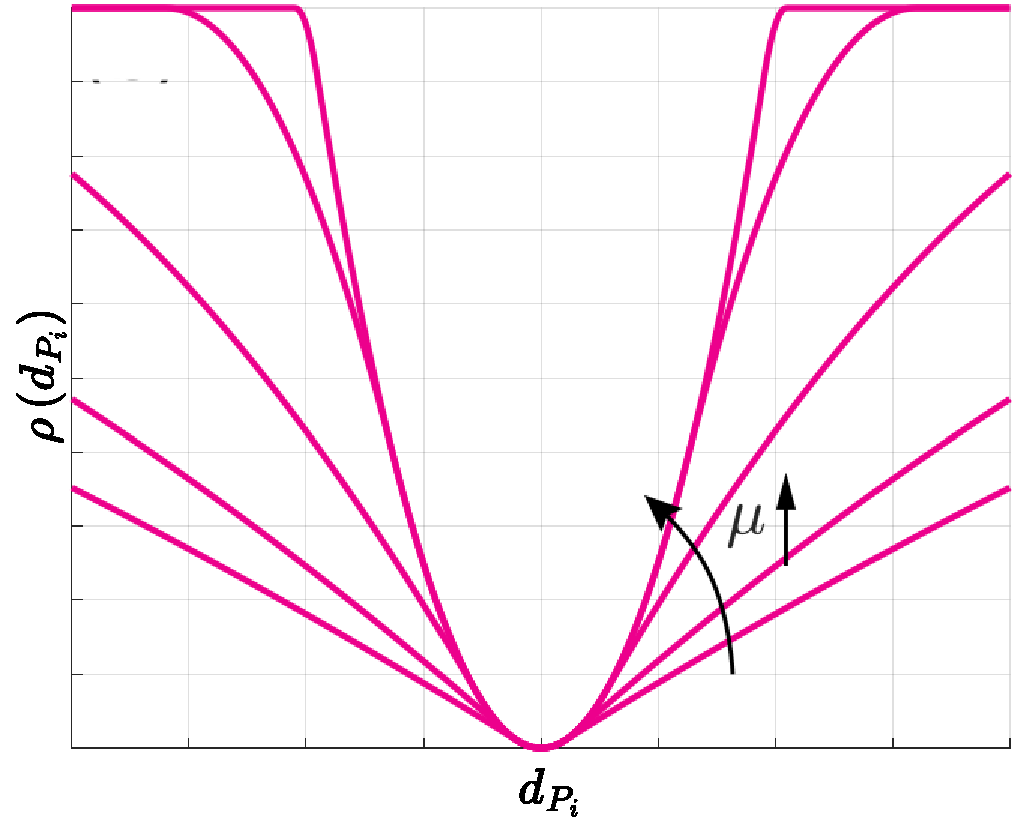
\includegraphics[width=0.3\textwidth]{chapters/2-pose-estimation/fig/tls-cost.pdf}
	\end{center}
	\caption{Cost function for the \gls{tls} with }
	\label{fig:tls-cost}
\end{figure}
\mvar{\bar{c}^2} is a given truncation threshold, which in practice is set to the maximum error expected for the inliers. Finally, \mvar{w_i} can be computed when using \gls{tls} by
%
\begin{equation}\label{eq:tls-weights}
	w_i^{(t)} = \begin{cases}
		0 & \text{ if } \hat{r}_i^2\in\left[ \frac{\mu+1}{\mu}\bar{c}^2, +\infty \right] \\
		\frac{\bar{c}}{\hat{r}_i}\sqrt{\mu(\mu+1)} - \mu & \text{ if } \hat{r}_i^2\in\left[ \frac{\mu}{\mu+1}\bar{c}^2, \frac{\mu + 1}{\mu}\bar{c}^2 \right] \\
		1 & \text{ if } \hat{r}_i^2\in\left[ 0, \frac{\mu}{\mu + 1}\bar{c}^2 \right] \\
	\end{cases}
\end{equation}
where \mvar{\hat{r}_i^2\overset{\cdot}{=} d_{P_i}(\cdot)^2}. \eqref{eq:br-result} can now be solved through a two-step alternating optimization. First, an outer loop is defined to which increases control parameter \mvar{\mu} from \num{0} to \mvar{\infty}, until a stop criterion, dictated by the cost function, is met.~\cite{graduated-non-convexity-for-robust-spatial-perception:-from-non-minimal-solvers-to-global-outlier-rejection} found that an increase of \mvar{\mu} by a factor of \num{1.4} provided satisfactory results.
The inner loop is two-fold 1) the current estimate of \tf[R]{(t)}{} is computed by optimizing over \tf[R]{}{} with fixed weights \mvar{w_i}, also referred to as the variable update step. The variable update step can thus be written as
%
\begin{equation}\label{eq:variable-update}
	\tf[R]{(t)}{} = \arg\min_{\mat{R}\in\SE (3)} \sum^N_{i=1}w_i^{(t-1)}d_{P_i}(\vec{x}_i,\mat{R}) + \underbrace{\Phi_{\rho_\mu}\left(w_i^{(t-1)}\right)}_{\text{constant}}
\end{equation}

This optimization problem is non-convex and is solved using \gls{rcqp}, which is described in~\secref{subs:2-pose-estimation-relaxed-convex-quadratic-programming}. 2) the found \tf[R]{}{} is then used to update the weights \mvar{w_i\forall i =1,2,\dots, N}, which typically can be solved in closed form, as formulated in~\eqref{eq:tls-weights}, which also is referred to as the weight update step. \medskip

When executing \gls{gnc} in practice, values are needed for \mvar{\mu_0} and \mvar{\vec{w}^(0)}, i.e. the parameters' initial values, along with an update rule for \mvar{\mu} and a stopping criterion. 
In this project the initial value for \mvar{\mu} is \mvar{\mu=2r_{\max}^2/\bar{c}^2} where \mvar{r_{\max}^2 \overset{\cdot}{=}\max_i \left(r^2(\vec{x}_i,\mat{R}^{(0)})\right)}, meaning the maximum residual after the first variable update, while \mvar{\vec{w}^{(0)}_i=1 \forall i=1,2,\dots,N}. The update rule used for \mvar{\mu} is \mvar{\mu\leftarrow 1.4\mu}, and as mentioned previously \mvar{\bar{c}^2} is set to the maximum error expected for the inliers. For \gls{tls} a fitting stop criterion is chosen to be the sum weighted squared residuals, i.e.
\begin{equation}
	\sum^N_{i=1}w_i\hat{r}_i^2.
\end{equation}
These initial values, update rules and stop criterion are based on the discoveries of~\cite{graduated-non-convexity-for-robust-spatial-perception:-from-non-minimal-solvers-to-global-outlier-rejection}. The \gls{gnc} algorithm can be seen summarized in~\algoref{alg:gnc}.

\begin{algorithm}
	\floatname{algorithm}{Algorithm}
	\algrenewcommand\algorithmicrequire{\textbf{Input: }}
	\algrenewcommand\algorithmicensure{\textbf{Output: }}
	\caption{\gls{gnc} algorithm when using \gls{tls} as \mvar{\rho(\cdot)}}
	\label{alg:gnc}
	\begin{algorithmic}[1]
		\Require matching pairs from (\mat{X},\mat{Y}) 
		\Ensure inliers, stats
		\While {true} // outer loop
			\State $\mu\gets 1.4\mu$
			\State $\mat{R}^{(t)} \gets $ Variable Update
			\State $\vec{w}^{(t)} \gets $ Weight Update
			\If{$\sum^N_{i=1}w_i\hat{r}_i^2$ has converged}
				\State \textbf{break}
			\EndIf
		\EndWhile
		\State \textbf{return} inliers, stats
	\end{algorithmic}
\end{algorithm}

In~\algoref{alg:gnc} the stats output generally contains information about the algorithm execution such as execution time, number of iterations, and the weights \vec{w}.

% \gls{gnc} refers to a phenomenon that arises in optimization problems where the objective function exhibits non-convexity and has multiple local optima. In contrast to traditional non-convex optimization, \gls{gnc} exploits the presence of these local optima to find better solutions progressively. \medskip

% To understand \gls{gnc}, let's start by defining some terms. In optimization, a convex function is one that has a unique global minimum. Mathematically, a function \mvar{f(\vec{x})} defined on a convex set \mat{X} is convex if for any two points \mvar{\vec{x}_1} and \mvar{\vec{x}_2} in \mat{X} and any $\lambda \in [0,1]$, the following inequality holds:
% \begin{equation}
% 	f(\lambda \vec{x}_1 + (1-\lambda)\vec{x}_2) \leq \lambda f(\vec{x}_1) + (1-\lambda)f(\vec{x}_2)
% \end{equation}

% This inequality essentially means that the function lies below the line segment connecting any two points on its graph. Convex optimization is a well-studied field with efficient algorithms for finding the global minimum.

% However, many real-world problems involve non-convex functions, which may have multiple local minima, saddle points, or other complex structures. Traditional optimization methods struggle with non-convex problems because they can get stuck in local optima, unable to find the global optimum.

% \gls{gnc} takes a different approach. Instead of trying to escape local optima, it leverages them to improve the optimization process. The idea is to gradually increase the level of non-convexity in the objective function during optimization. This process allows the algorithm to refine its solution by escaping local optima at a controlled pace.

% A common technique used in GNC is to introduce a parameter $t$ that controls the level of non-convexity. As \mvar{t} increases, the objective function becomes more non-convex. The optimization algorithm starts with a low value of $t$ where the objective function is approximately convex. It then gradually increases $t$ over time, exploring the non-convex landscape.

% The introduction of $t$ is often done by incorporating a regularization term into the objective function. The regularization term helps to maintain the properties of the convex function, ensuring that the optimization algorithm does not diverge. As $t$ increases, the regularization term becomes less significant compared to the non-convex part of the objective function, allowing the algorithm to escape local optima.

% A common form of the objective function in GNC is:

% \begin{equation}
% 	F_t(x) = f(x) + t\phi(x)
% \end{equation}

% where $f(x)$ is the original non-convex function to be optimized, $\phi(x)$ is a convex regularization term, and $t$ is the parameter controlling the non-convexity level.

% The choice of the regularization term $\phi(x)$ depends on the problem at hand and the desired behavior of the optimization algorithm. It should be designed in such a way that it encourages exploration of the non-convex landscape as $t$ increases.

% During the optimization process, as $t$ gradually increases, the algorithm starts with a nearly convex objective and finds a solution that is close to a local optimum. Then, it gradually explores the non-convex landscape by increasing the influence of the non-convex part of the objective function. This exploration helps the algorithm find better solutions that are not trapped in local optima.

% In summary, Graduated Non-Convexity is a technique used in optimization problems with non-convex objective functions. It gradually increases the level of non-convexity to explore the landscape and escape local optima. By incorporating a regularization term that maintains convexity at

% Let's consider a specific optimization problem with a non-convex objective function $f(x)$ that we want to minimize. We introduce a parameter $t$ to control the level of non-convexity.

% First, let's define the problem in a matrix and vector form. Suppose we have a vector of variables $x \in \mathbb{R}^n$ and a matrix $A \in \mathbb{R}^{m \times n}$ representing the problem's constraints. The optimization problem can be formulated as:

% \begin{align*}
% \text{minimize} & \quad f(x) \\
% \text{subject to} & \quad Ax \leq b,
% \end{align*}

% where $b \in \mathbb{R}^m$ is the vector of constraint values.

% To incorporate Graduated Non-Convexity, we introduce a convex regularization term $\phi(x)$ that helps maintain the properties of a convex function. The objective function $F_t(x)$ becomes:

% \begin{equation}
% 	F_t(x) = f(x) + t\phi(x).
% \end{equation}


% Here, $t$ controls the level of non-convexity, and as $t$ increases, the influence of the non-convex part ($t\phi(x)$) becomes more significant.

% For example, let's consider a simple case where $f(x)$ is a quadratic function and $\phi(x)$ is a convex regularization term. We can express $f(x)$ using a matrix form as:

% \begin{equation}
% 	f(x) = \frac{1}{2} x^T Q x + c^T x,
% \end{equation}

% where $Q \in \mathbb{R}^{n \times n}$ is a symmetric positive semi-definite matrix, and $c \in \mathbb{R}^n$ is a vector.
% The convex regularization term $\phi(x)$ can be written as:

% \begin{equation}
% 	\phi(x) = g(Dx),
% \end{equation}

% where $D \in \mathbb{R}^{p \times n}$ is a matrix, and $g(\cdot)$ is a convex function.

% The objective function $F_t(x)$ with GNC can be written as:

% \begin{equation}
% 	F_t(x) = \frac{1}{2} x^T Q x + c^T x + t g(Dx).
% \end{equation}

% Now, during the optimization process, we start with a small value of \mvar{t} e.g., \mvar{t = 0} where the objective function is approximately convex. We solve the optimization problem using traditional convex optimization techniques, such as quadratic programming, to find a solution \mvar{x_0} that is close to a local optimum.

% Then, we gradually increase \mvar{t} over time, which increases the non-convexity of the objective function. As \mvar{t} increases, the regularization term becomes less significant compared to the non-convex part \mvar{t g(Dx)}, allowing the algorithm to explore the non-convex landscape and potentially escape local optima.

% The specific choice of the convex regularization term \mvar{\phi(x)} and the function \mvar{g(\cdot)} depends on the problem at hand. Common choices include the \mvar{\ell_1} norm, total variation, or other convex functions that encourage certain properties or structures in the solution.

% In summary, the math behind Graduated Non-Convexity involves introducing a parameter \mvar{t} to control the level of non-convexity and incorporating a convex regularization term \mvar{\phi(x)}


% Step 1: Initialize the algorithm

% \begin{align*}
% &\text{Set } t = t_0 \text{ initial value of } t \\
% &\text{Set } x_0 \text{ as an initial feasible solution} \\
% &\text{Set iteration counter } k = 0
% \end{align*}


% Step 2: Solve the convex subproblem

% \begin{align*}
% &\text{Solve the following convex subproblem to obtain a solution } x_k: \\
% &\quad \min_{x} \frac{1}{2}x^TQx + c^Tx \\
% &\quad \text{subject to } Ax \leq b
% \end{align*}

% Step 3: Update the parameter \mvar{t}
% % \begin{align*}
% % &\text{Update } t \text{ based on a predefined schedule, e.g., } t = g(k) \text{ for some function } g(\cdot) \\
% % &\text{Increment } k \text{ by 1 (} k = k + 1\text{)}
% % \end{align*}

% Step 4: Update the objective function

% \begin{align*}
% &\text{Compute the convex regularization term: } \phi(x_k) \\
% &\text{Update the objective function with the increased non-convexity: } \\
% &\quad F_t(x) = \frac{1}{2}x^TQx + c^Tx + t\phi(x)
% \end{align*}

% Step 5: Solve the updated non-convex problem

% \begin{align*}
% &\text{Solve the following non-convex problem to obtain a new solution } x_{k+1}: \\
% &\quad \min_{x} F_t(x)
% \end{align*}

% Step 6: Check termination criteria

% \begin{align*}
% &\text{If termination criteria are satisfied, stop and return the current solution } x_{k+1} \\
% &\text{Otherwise, go to Step 3}
% \end{align*}

% In Step 2, the convex subproblem represents a traditional convex optimization problem that can be solved using various techniques such as quadratic programming or linear programming.

% In Step 4, the convex regularization term $\phi(x_k)$ can take different forms based on the problem requirements. For example, if $\phi(x_k)$ is based on the $\ell_1$ norm, it can be computed as $\phi(x_k) = \|Dx_k\|_1$ where $D$ is a matrix that determines the sparsity pattern.

% In Step 6, the termination criteria can be defined based on the problem's requirements or convergence properties, such as reaching a maximum number of iterations, achieving a desired objective value, or satisfying certain optimality conditions.

% The algorithm iteratively solves a sequence of convex subproblems and updated non-convex problems, gradually increasing the non-convexity level with the parameter \mvar{$t$}. By exploring the non-convex landscape, the algorithm aims to escape local optima and find better solutions.

% Remember that the specific implementation details of the GNC algorithm may vary depending on the problem, the chosen convex regularization term, and the optimization techniques used in solving the convex subproblems.

\subsection{Relaxed Convex Quadratic Programming} \label{subs:2-pose-estimation-relaxed-convex-quadratic-programming}

% Chapter: Tight Dual Relaxation for Non-Convex Optimization

To compute the optimal rotation matrix \tf[R]{}{}, the problem definition must be expressed purely in \tf[R]{}{}. To do so, it will be derived from the optimization problem involving the full transformation matrix \tf[T]{}{}, formulated as
%
\begin{equation}\label{eq:linear-in-r-and-t}
	d_{P_i}^2(\vec{x}_i, \mat{T})=(\mat{T}\oplus \vec{x}_i - \vec{y}_i)^\T\mat{C}_i (\mat{T}\oplus \vec{x}_i - \vec{y}_i).
\end{equation}
Here \mvar{\mat{T}\oplus \vec{x}_i} is the Euclidean transformation of \mvar{\vec{x}_i}, which is an expression linear in \tf[R]{}{} and \vec{t}
%
\begin{equation}
	\tf[T]{}{} \oplus \vec{x}_i = \mat{R}\vec{x}_i + \vec{t} = \left( \tilde{\vec{x}}^\T \otimes \mat{I}_3\right) \text{vec}(\mat{T}).
\end{equation}
Here \mvar{\tilde{\vec{x}}=\rvec{\vec{x}^\T, 1}^\T} is the homogeneous coordinate of \vec{x}, \mvar{\otimes} is the Kronecker product and \mvar{\text{vec}(\mat{T})} is the vectorization of \mat{T} i.e.
%
\begin{align}
	\text{vec}(\mat{T}) &= \rvec{\text{vec}(\mat{R})^\T, \vec{t}^\T}^\T \\
	&= \rvec{r_{11},r_{12},\dots,r_{32},r_{33},t_{1},t_{2},t_{3}}^\T.
\end{align}
Using this linear relationship in \mat{T},~\eqref{eq:linear-in-r-and-t} can be reformulated as 
%
\begin{equation}\label{eq:quadratic-nature}
	d_{P_i}(\vec{x}_i,\mat{T})=\tilde{\vec{\tau}}^\T \mat{N}_i^\T \mat{C}_i \mat{N}_i \tilde{\vec{\tau}}
\end{equation}
where \mvar{\vec{\tau}} is \mvar{\text{vec}(\mat{T})}, \mvar{\tilde{\vec{\tau}}} is the homogenized \mvar{\text{vec}(\mat{T})} i.e. \mvar{\rvec{\text{vec}(\mat{T})^\T,1}^\T}, and \mvar{\mat{N}_i=\rvec{\tilde{\vec{x}}_i^\T \otimes \mat{I}_3 | -\vec{y}_i }\inR{3\times 10}}. Due to the quadratic nature of~\eqref{eq:quadratic-nature}, it is possible to organize the observations and compress all the data into a single matrix \mvar{\tilde{\mat{M}}} from \mvar{\tilde{\mat{M}}_i = \mat{N}_i^\T \mat{C}_i \mat{N}_i\inR{13\times 13}}
%
\begin{equation}
	f(\mat{T})=\sum^N d_{P_i}(\vec{x}_i,\mat{T})=\tilde{\vec{\tau}}^\T \left( \sum^N_{i=1} \tilde{\mat{M}}_i \right) \tilde{\vec{\tau}} = \tilde{\vec{\tau}}^\T \tilde{\mat{M}} \tilde{\vec{\tau}}.
\end{equation}
From this expression, it can now be seen that the problem has been made independent of \mvar{N}. By then applying marginalization to the unconstrained parts of the known \mat{T} i.e. the translation \vec{t}, further compression of the problem is achieved, such that
%
\begin{equation}\label{eq:prep-primary-problem}
	f^\star = \min_{\mat{R}\in \SE (3)} \tilde{\vec{r}}^\T \tilde{\mat{Q}} \tilde{\vec{r}} \qquad, \qquad \tilde{\vec{r}}=\rvec{\text{vec}(\mat{R})^\T, 1}^\T
\end{equation}
Here \mvar{\tilde{\mat{Q}}} is the Schur complement of the block matrix \mvar{\tilde{\mat{M}}_{t,t}} in \mvar{\tilde{\mat{M}}}. Here the \mvar{t} subscript indicates the indexes of the corresponding to translation variables and
\begin{equation}
	\mat{Q} = \tilde{\mat{M}}_{!t,!t} - \tilde{\mat{M}}_{!t,t}\tilde{\mat{M}}_{t,t}\inv \tilde{\mat{M}}_{t,!t}
\end{equation}
with \mvar{!t} being the complement of \mvar{t}.\medskip 

Although the problem is originally non-convex, it is approached by applying a convex relaxation technique to facilitate its solution. Although a formal proof is not presented, empirical evidence from~\cite{convex-global-3d-registration-with-lagrangian-duality} demonstrates that this relaxation method consistently produces results that are close to the globally optimal solution for the marginalized problem. \medskip

This convex relaxation is achieved by applying Lagrangian duality to define two problems, a primary problem~\ref{eq:P} and a dual problem~\ref{eq:D}. The primary problem is an extension of~\eqref{eq:prep-primary-problem}, such that the necessary constraints for legal rotation matrices solutions are enforced, while the dual problem will be corresponding to a homogeneous version of the primal problem \ref{eq:P}, which makes~\ref{eq:D} a Semidefinite Program (SDP), meaning the problem is convex and can be solved using off the shelf solvers. \medskip

To apply Lagrangian duality, strong duality must hold between~\ref{eq:P} and~\ref{eq:D}, meaning the solution to each of the problems are equal and their objective function values coincide. While this is not proven to hold, empirically this relaxation appears always to be tight, meaning strong duality holds, even under extreme conditions as asserted by~\cite{convex-global-3d-registration-with-lagrangian-duality}. This project will continue under the assumption that strong duality holds. \medskip

To formulate~\ref{eq:P}, the constraints of \mvar{\mat{R}\in \SE (3)} state that orthonormality and positive unit determinant must hold i.e.
%
\begin{equation}
	\mat{R}^\T\mat{R} = \mat{I}_3 \qquad \text{and} \qquad \det(\mat{R})=+1
\end{equation}

While it is appealing to formulate~\ref{eq:P} as a \gls{qcqp}, the determinant constraint is cubic and thus does not allow this formulation. In other solutions to this problem, it is not uncommon to discard the determinant constraint~\cite{lagrangian-duality-in-3d-slam:-verification-techniques-and-optimal-solutions,planar-pose-graph-optimization:-duality-optimal-solutions-and-verification} resulting in the problem only being constrained by the orthonormality constraint. This amounts to optimizing in O(3) rather than in SO(3). \medskip

Instead, by introducing additional constraints, the duality of the problem can be enhanced. Each time a new scalar constraint $c_{k+1}(\cdot)$ is incorporated into the Lagrangian, a corresponding dual variable $\lambda_{k+1}$ is introduced, and the dimension of the dual problem increases by one. This causes the new \ref{eq:D} bound \mvar{d^\star_{k+1}} to be at least as good as the previous problem's bound i.e.
%
\begin{equation}
	d^\star_{k} \le d^\star_{k+1} \le f^\star.
\end{equation}
Since this change in \ref{eq:P} causes direct changes to \ref{eq:D}, \ref{eq:D} is not intrinsic, instead it is dependant on the feasible region of \ref{eq:P}. By utilizing this property, adding more valid quadratic constraints has been shown to improve the quality of the dual relaxation~\cite[Chapter 13]{semidefinite-programming-relaxations-of-nonconvex-quadratic-optimization}. \medskip

Thus additional linearly independent quadratic constraints are added such as column and row-based orthonormality, along with additional quadratic constraints, which enforce the positive unit determinant, referred to as the rotation matrices handedness. This constraint states that a positive unit determinant is guaranteed if the column space of \mat{R} respects the right-hand rule i.e.
%
\begin{equation}
	\mat{R}^{(1)}\times \mat{R}^{(2)} = \mat{R}^{(3)},
\end{equation}
where \mvar{\mat{R}^{(k)}} is the $k$-th column of \mat{R}. Utilizing the three possible cyclic permutations of this equation provides exactly three independent quadratic constraints, which strengthens the duality between \ref{eq:P} and \ref{eq:D}. A final constraint can be added by homogenizing~\ref{eq:P} by introducing an auxiliary variable $y$ with the constraint $y^2 = 1$. The primary problem~\ref*{eq:P} can thus be expressed as
%
\begin{align*}
	&\min_{\mat{R}\in \SE (3)} \tilde{\vec{r}}^\T \tilde{\mat{Q}} \tilde{\vec{r}}  \quad , \quad \tilde{\vec{r}}=\rvec{\text{vec}(\mat{R})^\T, y}^\T, \\
	& \text{s.t. }         \\ 
	&\qquad \qquad \mat{R}^\T\mat{R} = y^2\mat{I}_3, \tag{$\mathcal{P}$} \label{eq:P}\\
	&\qquad \qquad \mat{R}\mat{R}^\T = y^2 \mat{I}_3, \\
	&\qquad \qquad \mat{R}^{(i)}\times \mat{R}^{(j)}=y \mat{R}^{(k)} \quad , \quad i,j,k = \text{cyclic}(1,2,3), \\
	&\qquad \qquad y^2 = 1.
\end{align*}

To derive the dual problem~\ref{eq:D}, the \gls{qcqp} nature of~\ref{eq:P} is utilized to express its Lagrangian as
%
\begin{equation}\label{eq:lagrangian-p}
	\mathcal{L}(\tilde{\vec{r}}, \tilde{\vec{\lambda}}) = \gamma + \tilde{\vec{r}}^\T  \tilde{\mat{Z}}  \tilde{\vec{r}}.
\end{equation}
Here \mvar{\tilde{\vec{\lambda}}=\rvec{\vec{\lambda}^\T, \gamma}^\T\inR{22}}, where \num{22} is the number of constraints of~\ref{eq:P}, \mvar{\tilde{\mat{Z}}=\tilde{\mat{Q}} + \tilde{\mat{P}}(\tilde{\vec{\lambda}})}, which is a penalization matrix as the sum of \mvar{\tilde{\mat{Q}}}, which contains all the data from~\ref{eq:P}, and \mvar{\tilde{\mat{P}}(\tilde{\vec{\lambda}})} is the accumulation of all the penalization terms corresponding to different constrain types. \mvar{\tilde{\mat{P}}(\tilde{\vec{\lambda}})} can be computed as
%
\begin{equation}\label{eq:penalty-matrix}
	\tilde{\mat{P}}(\tilde{\vec{\lambda}}) = \tilde{\mat{P}}_r(\mat{\Lambda}_r) + \tilde{\mat{P}}_c(\mat{\Lambda}_c) + \tilde{\mat{P}}_d(\{ \vec{\lambda}_{d_{ijk}} \}) + \tilde{\mat{P}}_h(\gamma),
\end{equation}
which by definition is a linear function of the dual variables, where the structural pattern of the involved matrices can be found in~\cite{convex-global-3d-registration-with-lagrangian-duality}. Using this formulation of the Lagrangian, its relaxation can be solved in closed form as 
\begin{align}
	d(\tilde{\vec{\lambda}})&=\min_{\tilde{\vec{r}}}\mathcal{L}(\tilde{\vec{r}},\tilde{\vec{\lambda}})=\min_{\tilde{\vec{r}}} \gamma + \tilde{\vec{r}}^\T \tilde{\vec{Z}} \tilde{\vec{r}} \\
	&= \begin{cases}
		\gamma & \text{ if } \tilde{\mat{Z}} \succeq \vec{0}, \\
		-\infty & \text{ otherwise }.
	\end{cases}
\end{align}
In cases where \mvar{\tilde{\mat{Z}}} is not \gls{psd} no lower bound exists for this problem, and thus no optimal solution can be found. But by restricting all \mvar{\tilde{\vec{\lambda}}}, to the solutions of \mvar{d(\tilde{\vec{\lambda}})} which satisfy \mvar{\tilde{\mat{Z}} \succeq \vec{0}}, the dual problem \ref{eq:D} to the homogeneous primal problem \ref{eq:P} is a Semidefinite Program on the form 
%
\begin{align*}
	& d^\star = \max_{\tilde{\vec{\lambda}}} \gamma, \\
	& \text{s.t. }         \tag{$\mathcal{D}$} \label{eq:D}\\ 
	&\qquad \qquad \tilde{\mat{Z}}(\tilde{\vec{\lambda}})=\tilde{\mat{Q}} + \tilde{\mat{P}}(\tilde{\vec{\lambda}}) \succeq 0. 
\end{align*}
Which is a semidefinite program i.e. a convex problem that can be solved by out-of-the-box solvers. \medskip

From the now defined primal problem~\ref{eq:P} and dual problem~\ref{eq:D}, and under the assumption that strong duality holds \mvar{f^\star = d^\star}, by duality theory \mvar{\tilde{\vec{r}}^\star} must be a minimizer of the Lagrangian~\ref{eq:lagrangian-p} evaluated at \mvar{\tilde{\vec{\lambda}}^\star}, such that
%
\begin{equation}
	\vec{r}^\star = \arg\min_{\vec{r}} \mathcal{L}(\vec{r},\vec{\lambda}^\star) \quad \Rightarrow \quad \left( \tilde{\vec{r}}^\star \right)^\T \tilde{\mat{Z}}^\star \tilde{\vec{r}}^\star = 0.
\end{equation}
Assuming \mvar{\tilde{\mat{Z}}^\star} is \gls{psd} i.e. \mvar{\tilde{\mat{Z}}^\star \succeq 0}, then the optimal solution \mvar{\tilde{\vec{r}}^\star} must lie in the nullspace of \mvar{\tilde{\mat{Z}}^\star} i.e. \mvar{\tilde{\vec{r}}^\star \in \text{null}\left( \tilde{\mat{Z}}^\star \right)}. If this was not the case, either \mvar{\text{null}\left( \tilde{\mat{Z}}^\star \right) = \emptyset} or \mvar{\tilde{\vec{r}}^\star \notin \text{null}\left( \tilde{\mat{Z}}^\star \right)}, as a direct consequence of \mvar{\tilde{\mat{Z}}^\star} being \gls{psd}. \medskip

Here the nullspace basis \mat{V} of \mvar{ \tilde{\mat{Z}}^\star } i.e. \mvar{\mat{V}=\text{null}\left( \tilde{\mat{Z}}^\star \right)} can be computed using QR decomposition. \medskip

If it here is the case that \mvar{\text{rank}(\mat{V})=1} then the optimal solution \mvar{\tilde{\vec{r}}^\star} is achieved up to a scaling factor of \mvar{1/y}, due to~\ref{eq:P} being homogenous. By simply dehomogenizing \mvar{\tilde{\vec{r}}^\star}, the optimal rotation \mvar{\vec{r}^\star} is found. \medskip

Verifying the legitimacy of this solution is simply done by evaluating the nullspace determinant to be unit, and the difference between the optimal value of~\ref{eq:P} and~\ref{eq:D} being \num{0} i.e.
%
\begin{equation}
	\text{rank} \left(\text{null}( \tilde{\mat{Z}}^\star )\right) = 1 \qquad \text{ and } \qquad  d^\star - f^\star(\vec{r}^\star) = 0
\end{equation}
where \mvar{\mat{R}^\star = \text{reshape}(\vec{r}^\star)}. \medskip

To summarize, the \gls{rcqp} algorithm can be seen in~\algoref{alg:rcqp}.

\begin{algorithm}
	\floatname{algorithm}{Algorithm}
	\algrenewcommand\algorithmicrequire{\textbf{Input: }}
	\algrenewcommand\algorithmicensure{\textbf{Output: }}
	\caption{\gls{rcqp} algorithm for determining \tf[R]{\star}{} from \mvar{\tilde{\vec{r}}^\T \tilde{\mat{Q}} \tilde{\vec{r}}}}
	\label{alg:rcqp}
	\begin{algorithmic}[1]
		\Require Marginalized quadratic form of the primary problem, \ref{eq:P} i.e. \mvar{\tilde{\vec{r}}^\T \tilde{\mat{Q}} \tilde{\vec{r}}}
		\Ensure Globally optimal \tf[R]{\star}{}, if strong duality holds
		\State \mvar{ \tilde{\mat{Z}} ( \tilde{\vec{\lambda}})  \gets } build\mvar{\left(\tilde{\mat{Q}} + \tilde{\mat{P}}(\tilde{\vec{\lambda}})\right)} based on~\ref{eq:penalty-matrix}

		\State \mvar{(\tilde{\vec{\lambda}}^\star, \tilde{\mat{Z}}^\star) \gets} \texttt{cvx}(\ref{eq:D}\mvar{(\tilde{\vec{\lambda}}, \tilde{\mat{Z}})}) i.e. solve the Semidefinite Program using optimization tools such as \texttt{cvx} 

		\State \mvar{\mat{V} \gets \text{null}(\tilde{\mat{Z}}^\star)}, from methods such as QR decomposition.

		\State \texttt{ASSERT} (rank\mvar{(\mat{V} ) == 1}), ensure the nullspace rank is unit
		\State \texttt{ASSERT} \mvar{\left( \left(\tilde{\vec{r}}^\star\right)^\T \tilde{\mat{Q}} \tilde{\vec{r}}^\star - d^\star < \epsilon \right)}  , where \mvar{\epsilon} is some threshold close to \num{0}, to ensure strong duality
		
		\State \mvar{\vec{r}^\star \gets \tilde{\vec{r}}^\star}, dehomogenize \mvar{\tilde{\vec{r}}^\star}

		\State \mvar{\tf[R]{\star}{} \gets} reshape(\mvar{\vec{r}^\star}), reshape \mvar{\vec{r}^\star\inR{9}} to \mvar{\mat{R}^\star\inR{3 \times 3}}
		\State \textbf{return} \tf[R]{\star}{}, return the globally optimal rotation
	\end{algorithmic}
\end{algorithm}

% While the problem remains non-convex, convex relaxation is applied to enable the solving of the problem. While no proof has been provided, this relaxation empirically proves to be tight in all the evaluated cases from~\cite{convex-global-3d-registration-with-lagrangian-duality}, enabling the recovery of a globally optimal solution for the marginalized problem.

% % 1. Introduction
% The tight dual relaxation method is a powerful approach for solving non-convex optimization problems. It leverages Lagrangian duality theory to obtain a globally optimal solution. This chapter provides an extensive explanation of the method presented in the paper, focusing on the mathematical formulations and key concepts involved. The sizes of vectors and matrices are explicitly mentioned to enhance clarity and understanding.

% % 2. Lagrangian Duality Basics
% Before delving into the tight dual relaxation method, it is essential to understand some fundamental concepts from Lagrangian duality theory. In Lagrangian duality, we consider an optimization problem with a primal objective function, subject to constraints. The Lagrangian function is formed by introducing dual variables associated with each constraint. The dual problem seeks to maximize the Lagrangian function over the feasible region defined by the dual variables. Duality theory establishes a relationship between the primal and dual problems, providing bounds on the optimal solutions.

% % 3. Problem Formulation
% Let's consider a non-convex optimization problem denoted as \mvar{P}. The objective is to find an optimal solution to this problem. The problem involves minimizing a cost function, subject to a set of constraints. The problem can be expressed as follows:

% \begin{align*}
% 	&\text{minimize } f(\vec{x}) \\
% 	& \text{subject to }         \\ 
% 	&\qquad \qquad g_i(\vec{x}) \leq 0, \quad i = 1, 2, \ldots, m \\
% 	&\qquad \qquad h_j(\vec{x}) = 0, \quad j = 1, 2, \ldots, p \\
% \end{align*}


% Here, \vec{x} represents the optimization variables, \mvar{f(\vec{x})} is the cost function, \mvar{g_i(\vec{x})} are the inequality constraints, and \mvar{h_j(\vec{x})} are the equality constraints.

% % 4. Lagrangian Dual Formulation
% To apply Lagrangian duality, we introduce dual variables \mvar{\lambda_i} for the inequality constraints and \mvar{\nu_j} for the equality constraints. The Lagrangian function for problem \mvar{P} is defined as:

% \begin{equation}
% 	L(\vec{x}, \lambda, \nu) = f(\vec{x}) + \sum_{i=1}^{m} \lambda_i g_i(\vec{x}) + \sum_{j=1}^{p} \nu_j h_j(\vec{x})
% \end{equation}


% Here, \mvar{\lambda = (\lambda_1, \lambda_2, \ldots, \lambda_m)} and \mvar{\nu = (\nu_1, \nu_2, \ldots, \nu_p)} are the vectors of dual variables.

% % 5. Lagrangian Dual Problem
% The Lagrangian dual problem seeks to maximize the Lagrangian function over the feasible region defined by the dual variables. The dual problem is formulated as follows:

% \begin{align*}
% 	 & \text{maximize } \theta(\lambda, \nu) = \inf_{x} L(x, \lambda, \nu) \\
% 	 & \text{subject to } \\
% 	 & \qquad \qquad \lambda \geq 0\\
% \end{align*}


% The function \mvar{\theta(\lambda, \nu)} represents the optimal value of the Lagrangian function.

% % 6. Tight Dual Relaxation Approach
% The tight dual relaxation approach aims to solve non-convex optimization problems by leveraging Lagrangian duality. The key idea is to formulate a dual problem that provides tight bounds on the optimal solution. In the tight dual relaxation, we carefully select the set of constraints to maximize the tightness of the relaxation.

% % 7. Primal Problem Formulation
% In the context of the paper, we consider a specific non-convex optimization problem denoted as \mvar{\tilde{P}}. The objective is to find an optimal 3x3

%  rotation matrix \mat{R} that satisfies orthonormality and determinant constraints. The primal problem \mvar{\tilde{P}} can be formulated as a Quadratically Constrained Quadratic Program (QCPQ):

% \begin{align*}
% 	& \text{minimize } \text{tr}(R^\top R - I)^2 \\
% 	& \text{subject to } \\
% 	& \quad\quad R^\top R = I \\
% 	& \quad\quad \text{det}(R) = 1
% \end{align*}


% Here, \mat{I} represents the identity matrix.

% % 8. Dual Problem Derivation
% To derive the dual problem for \mvar{\tilde{P}}, we construct the Lagrangian function \mvar{L(\mat{R}, \Lambda)}, where \mat{R} is the rotation matrix and \mvar{\Lambda} represents the dual variables associated with the constraints. The Lagrangian function is defined as:

% \begin{equation}
% 	L(R, \Lambda) = \text{tr}(\mat{R}^\top \mat{R} - \mat{I})^2 + \text{tr}(\Lambda^\top (R^\top \mat{R} - I)) + \lambda(\text{det}(\mat{R}) - 1)
% \end{equation}


% Here, \mvar{\Lambda} represents a symmetric matrix of dual variables and \mvar{\lambda} is a scalar dual variable.

% % 9. Penalized Matrix
% The tight dual relaxation approach involves constructing a penalized matrix to incorporate the penalization terms corresponding to the different kinds of constraints. The penalized matrix is denoted as \mvar{\mathcal{M}} and defined as:

% \begin{equation}
% 	\mathcal{M} = 2(R^\top R - I) + \Lambda + \lambda(I - R^\top R)
% \end{equation}


% Here, \mvar{\mathcal{M}} is a 3x3 matrix, \mvar{R^\top R} is a 3x3 matrix representing the orthonormality constraints, and \mvar{I} is the identity matrix.

% % 10. Lagrangian Relaxation
% The Lagrangian relaxation involves expressing the dual problem as an unconstrained problem by eliminating the equality constraints. The dual problem can be reformulated as follows:

% \begin{equation}
% 	\text{maximize } \mathcal{D}(\Lambda, \lambda) = \inf_{R} L(R, \Lambda, \lambda)
% \end{equation}

% Here, \mvar{\mathcal{D}(\Lambda, \lambda)} represents the optimal value of the Lagrangian function after relaxation.

% % 11. Dual Bound Function
% The tight dual relaxation provides a dual bound function \mvar{d(\lambda)} that estimates the optimal value of the primal problem. The dual bound function is defined as:

% \begin{equation}
% 	d(\lambda) = \max_{\Lambda} \mathcal{D}(\Lambda, \lambda)
% \end{equation}


% Here, \mvar{d(\lambda)} represents the dual bound.

% % 12. Conclusion
% The tight dual relaxation method is a powerful technique for solving non-convex optimization problems. By carefully selecting the set of constraints and formulating the dual problem, this method provides tight bounds on the optimal solution. The Lagrangian relaxation and dual bound function play crucial roles in the process. Understanding and applying the tight dual relaxation approach can lead to efficient and effective solutions to challenging optimization problems.

% % Note: This chapter provides a general explanation of the method based on the information available. For a more detailed and accurate understanding, it is recommended to refer to the original paper.



\section{Experimental Setup}\label{sec:2-pose-estimation-experimental-setup}

To Test the performance of the algorithms presented in~\secref{sec:2-pose-estimation-method} synthetic source data is generated based on the target data sampled from \gls{cad} model of the object of interest i.e. the Stanford bunny. The mesh is sampled uniformly with \num{1000} data points and with corresponding normals making up the target data, while the source data is made from a homogeneous transformation matrix applied to a copy of the target data. This will ensure the index \mvar{i} of each point in each point cloud will be true correspondences even when transformation. The homogeneous transformation matrix chosen is
\begin{equation}
	\tf[T]{\text{Target}}{\text{Source}} = 
	\begin{bmatrix}
		\tf[R]{}{z}(\pi/4) & \vec{t}_x(1) \\
		\vec{0}_{1\times 3} & 1
	\end{bmatrix}\inR{4\times 4}
\end{equation} 
where \mvar{\mat{R}_z(\pi/4)\inR{3\times 3}} is the rotation matrix for a rotation of \mvar{\pi/4=45\deg} about the $z$-axis, \mvar{\vec{t}_x(1)\inR{3}} is a translation along the $x$-axis of \num{1} and \mvar{\vec{0}_{1\times 3}=\rvec{0,0,0}}. The target and synthetic source data can be seen in \figref{fig:synthetic-target-data} and~\figref{fig:synthetic-source-data} respectively.

\begin{figure}[!h]
	\centering
	\begin{subfigure}[b]{0.48\textwidth}
		\centering
		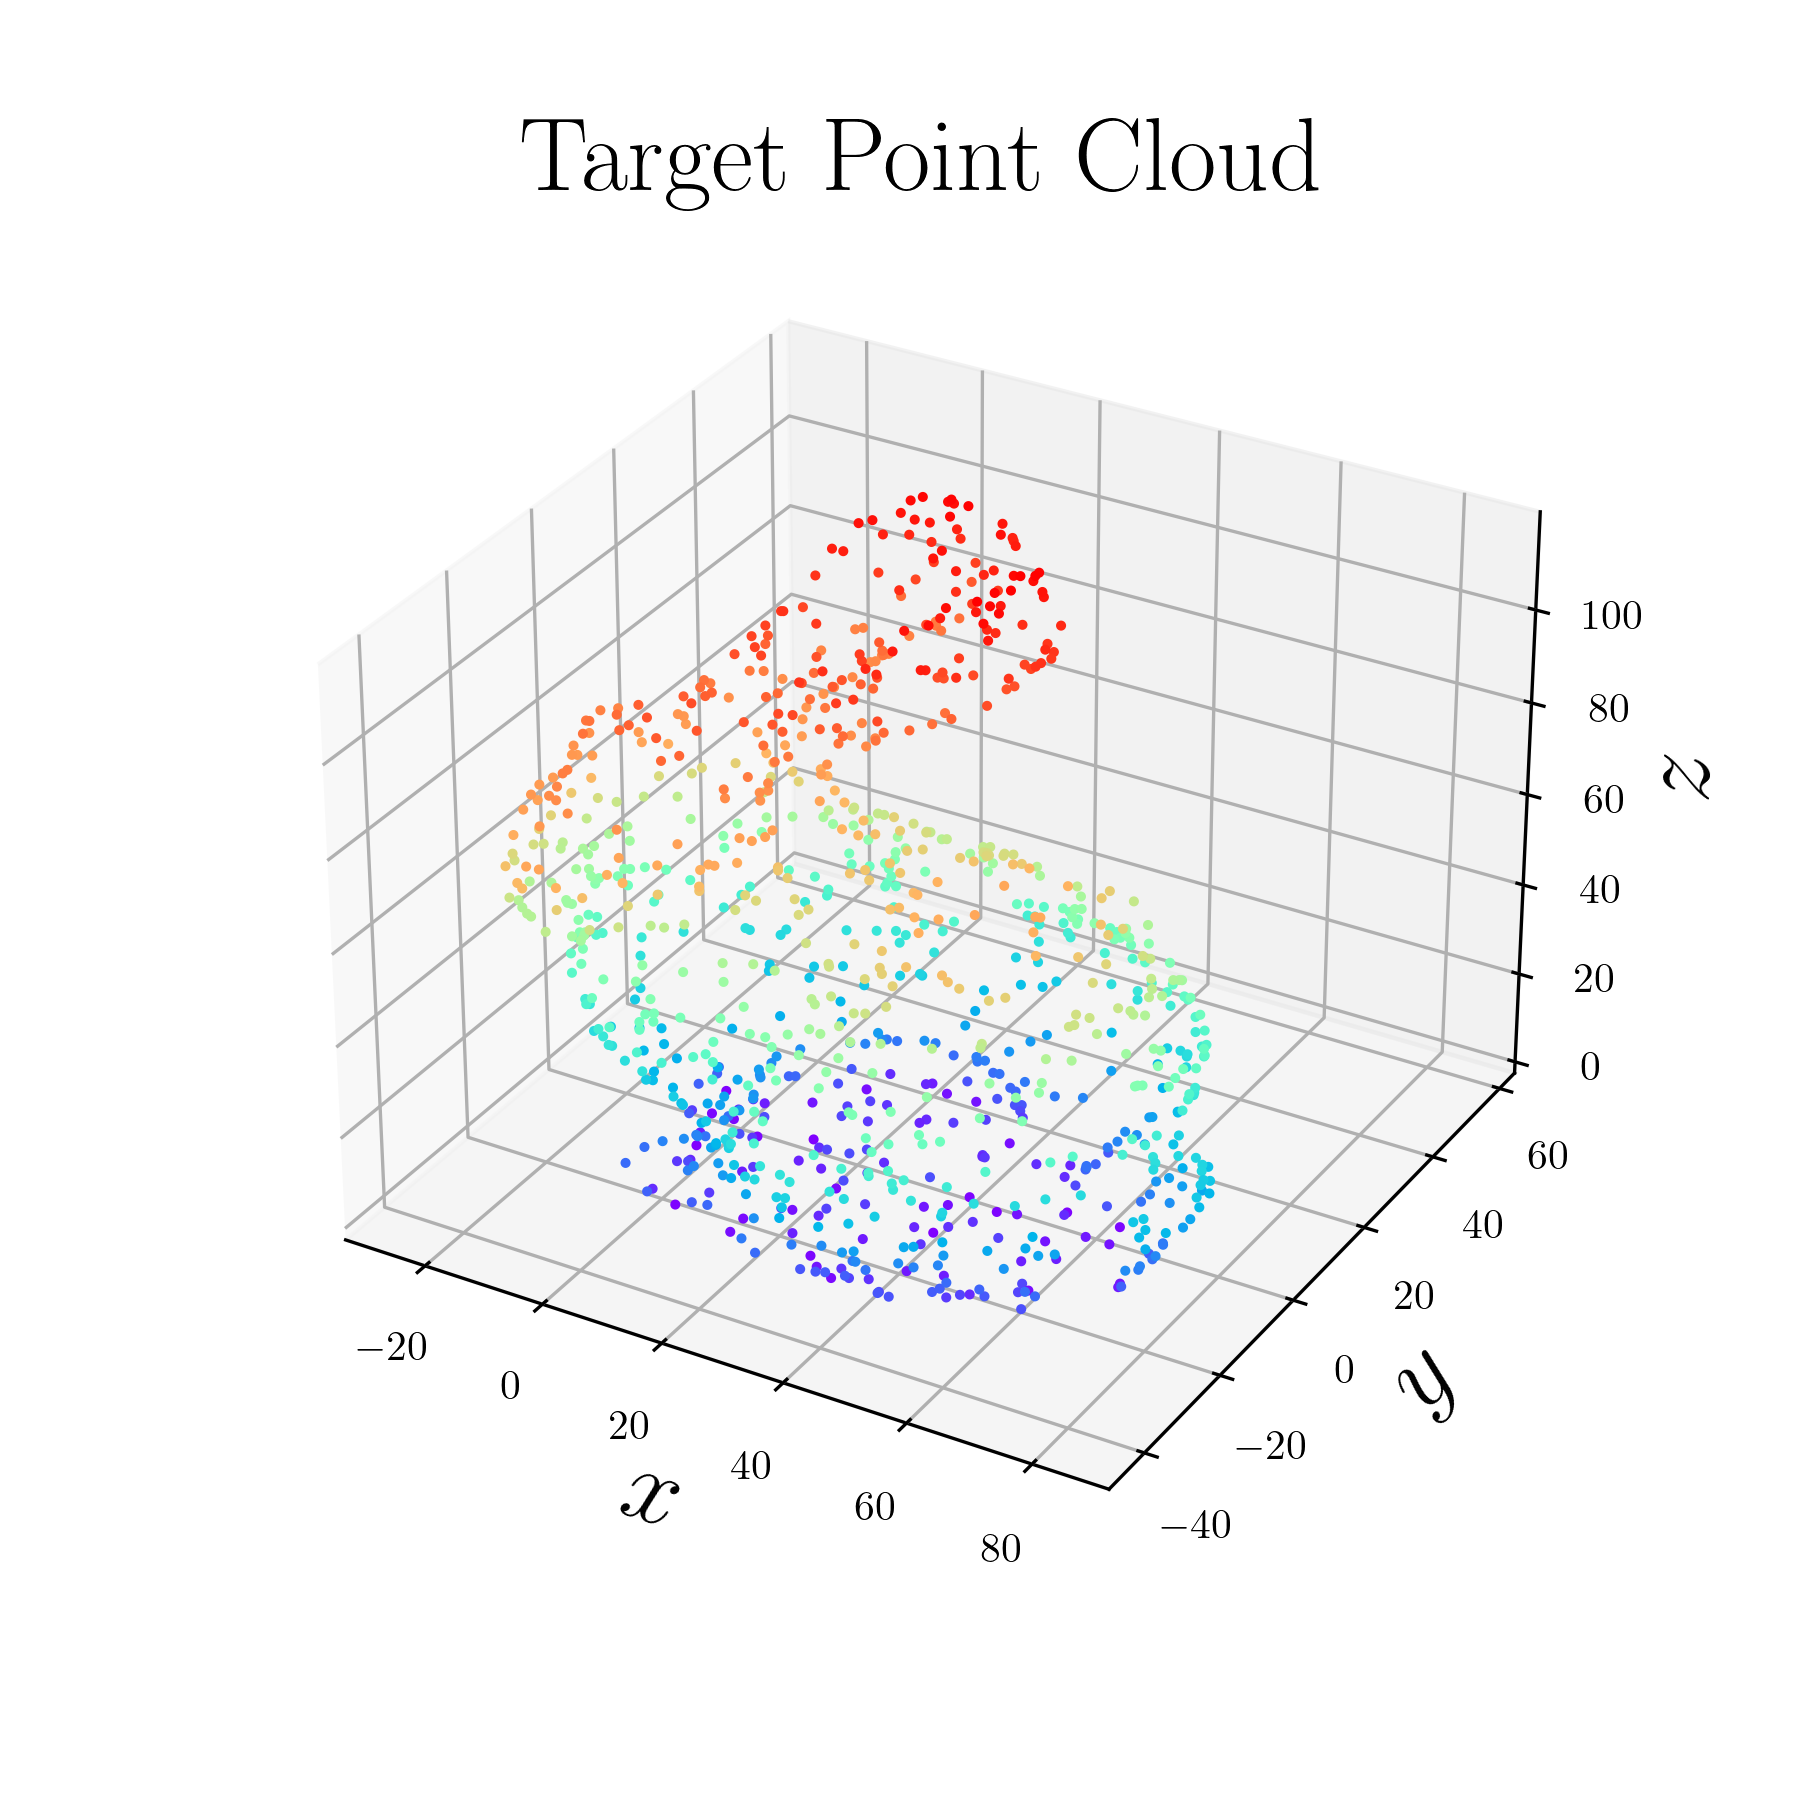
\includegraphics[width=\textwidth]{chapters/2-pose-estimation/fig/synthetic_pc_target.png}
		\caption{The target \gls{pc} generated from sampling \num{1000} points from the \gls{cad} model.}
		\label{fig:synthetic-source-data}
	\end{subfigure}
	\hfill
	\begin{subfigure}[b]{0.48\textwidth}
		\centering
		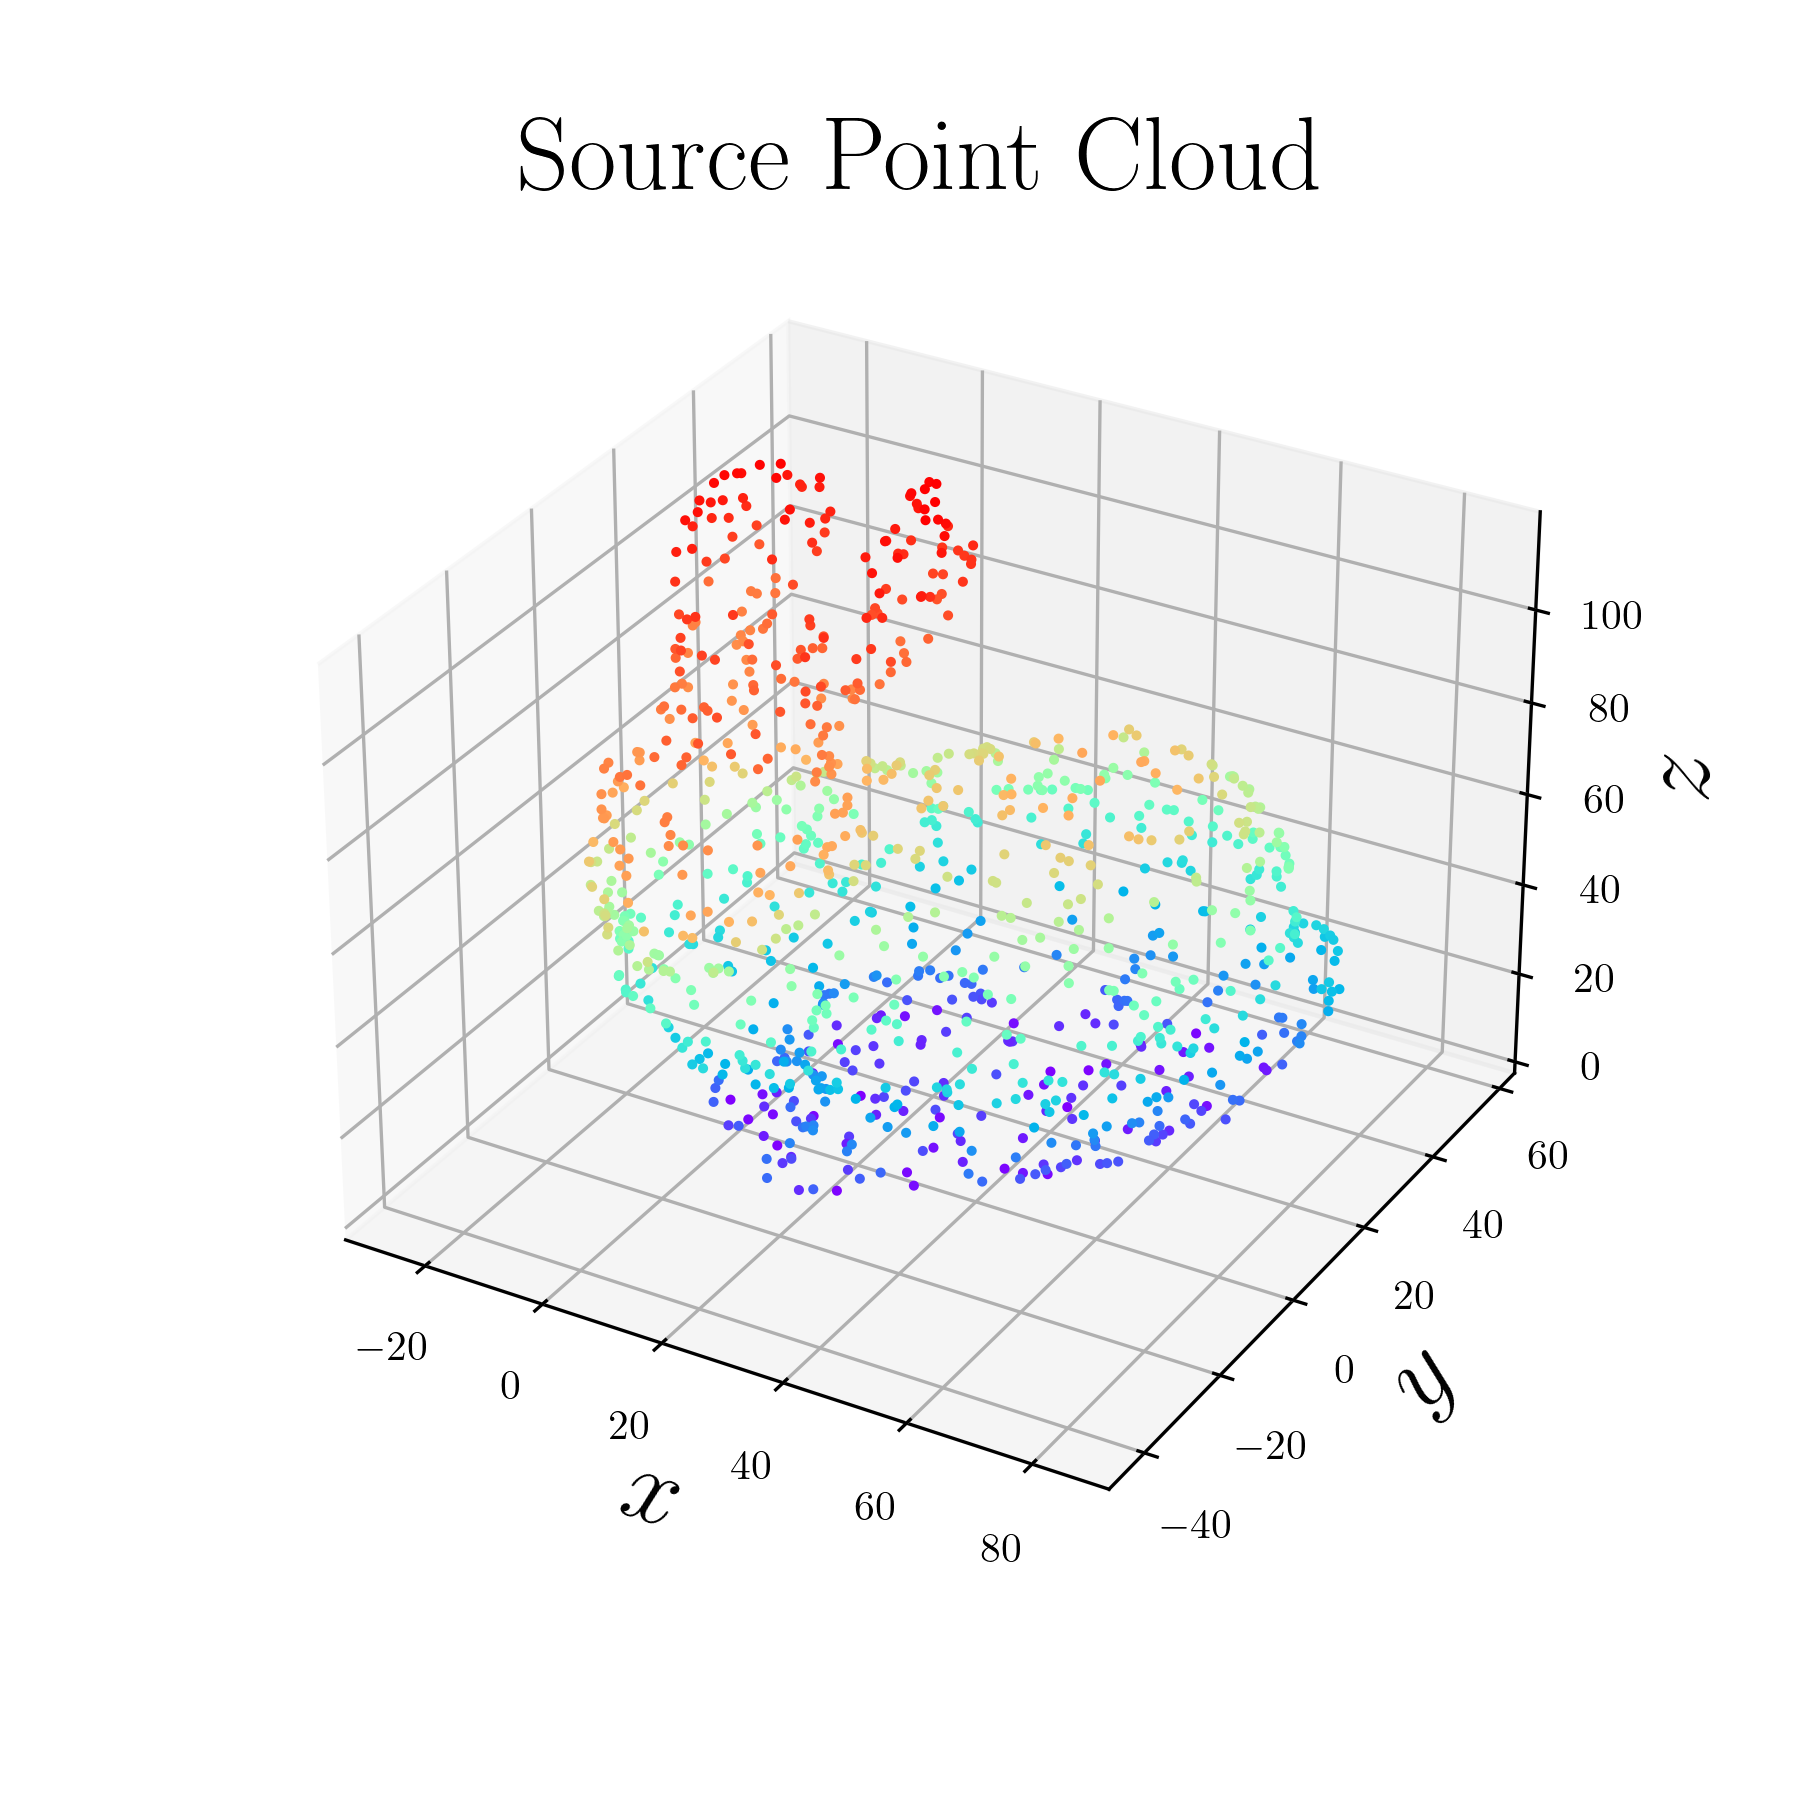
\includegraphics[width=\textwidth]{chapters/2-pose-estimation/fig/synthetic_pc_source.png}
		\caption{The synthetic source data based on the target data, but transformed \mvar{\tf[T]{\text{Target}}{\text{Source}}}.}
		\label{fig:synthetic-target-data}
	\end{subfigure}
	\caption{3D plots showing the synthetic source data and target data.}
	\label{fig:synthetic-source-and-target-data}
\end{figure}

On these points clouds \gls{gnc}+\gls{rcqp} are applied over \num{20} experiments with varying outlier percentages \mvar{\alpha=\rvec{10\%,20\%,\dots,90\%}}. \medskip

Once results are found, the method is applied to the sampled data shown in~\figref{fig:pe-pc-source}. This however includes the solving of the \gls{corr-problem} by finding feature correspondences between the point cloud. Due to self-collisions during the sampling process, a statistical outlier filter was applied with the number of neighbors \mvar{n_{nb}} being \num{1,000} and the standard deviation ratio \mvar{\sigma} being \num{0.5}.\medskip

Using \gls{fpfh} it was unfortunately found that the source data did not contain enough information to find a satisfactory number of feature matches with the target data for \gls{gnc}+\gls{rcqp} to function. This was found by sampling target data with a varying number of data points uniformly distributed while computing the number of feature matches with the sampled source data. These results can be seen in~\figref{fig:number-of-feature-matches-with-different-numbers-of-target-data-points}, where the number of target data points sampled are \mvar{\gamma = \rvec{100,200,\dots,900,1000,2000,\dots,50000}} and the largest number of feature matches show to be two, which is far from sufficient. Filtering the sampled source data did not increase the number of feature matches as shown in the figure.

\begin{figure}[!h]
	\begin{center}
		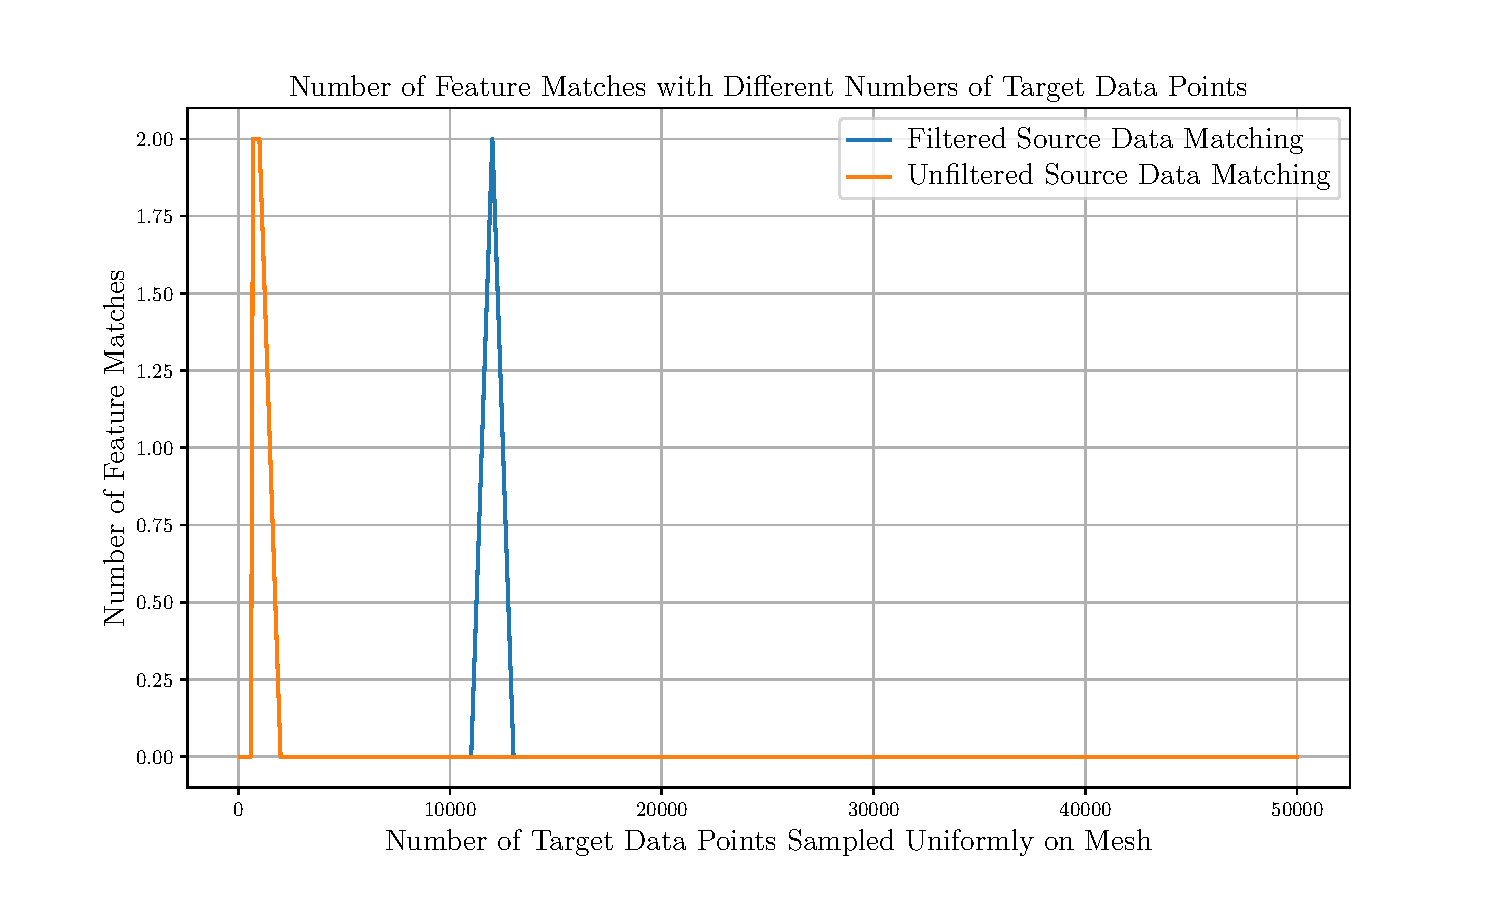
\includegraphics[width=0.8\textwidth]{chapters/2-pose-estimation/fig/number-of-feature-matches-with-different-numbers-of-target-data-points.pdf}
	\end{center}
	\caption{Number of feature matches between target data containing \mvar{\gamma} data points and the sampled source data, both filtered and unfiltered.}
	\label{fig:number-of-feature-matches-with-different-numbers-of-target-data-points}
\end{figure}
% Using these two, heatmaps were produced, where~\figref{fig:pe-feature-filtered-pc} shows the heatmap for the filtered source data while~\figref{fig:pe-feature-unfiltered-pc} shows the heatmap for the unfiltered source data. \medskip
% \begin{figure}[!h]
% 	\centering
% 	\begin{subfigure}[b]{0.48\textwidth}
% 		\centering
% 		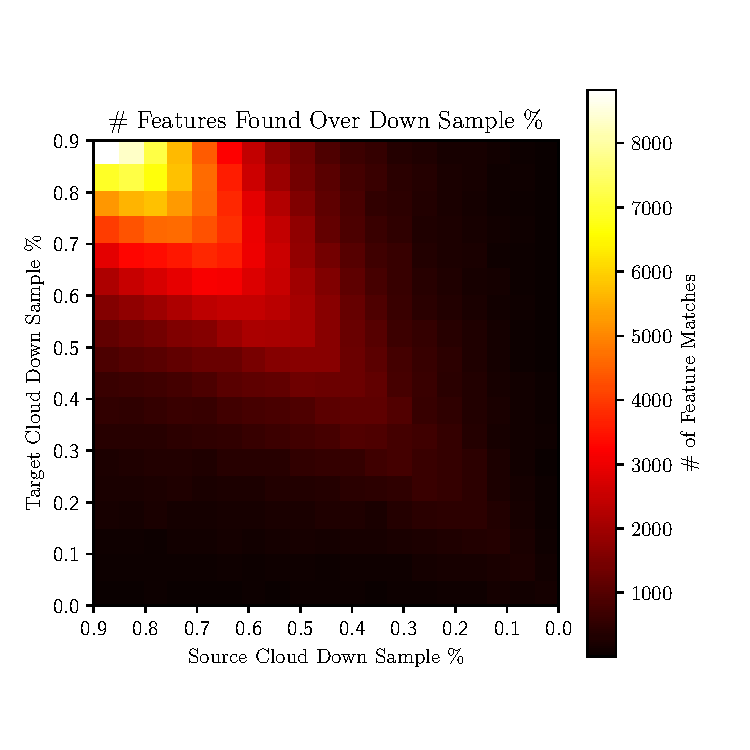
\includegraphics[width=\textwidth]{chapters/2-pose-estimation/fig/M.pdf}
% 		\caption{The source \gls{pc} generated from simulated contact points.\newline}
% 		\label{fig:pe-feature-filtered-pc}
% 	\end{subfigure}
% 	% \hfill
% 	\begin{subfigure}[b]{0.48\textwidth}
% 		\centering
% 		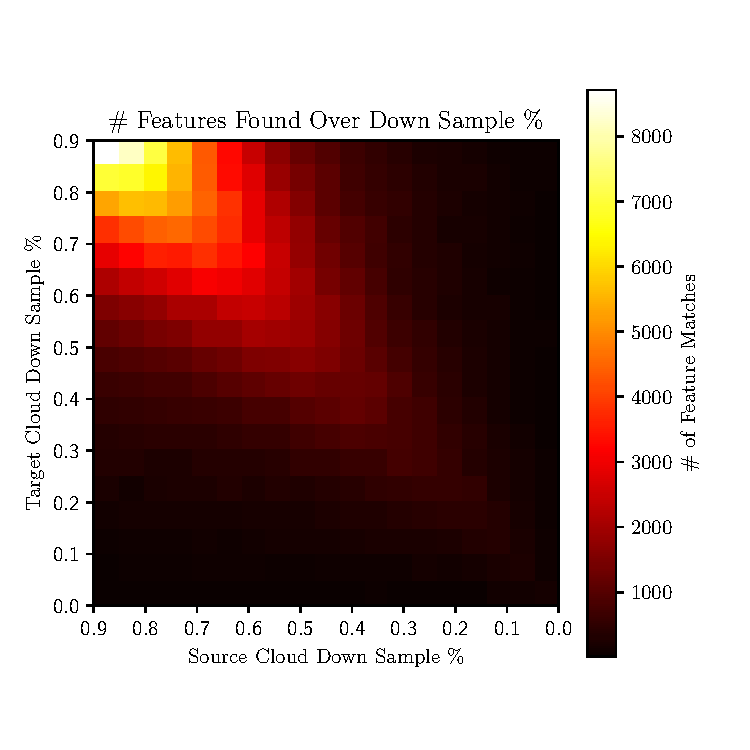
\includegraphics[width=\textwidth]{chapters/2-pose-estimation/fig/M_unfiltered.pdf}
% 		\caption{The target \gls{pc} generated by sampling the model mesh with \num{10,000} points.}
% 		\label{fig:pe-feature-unfiltered-pc}
% 	\end{subfigure}
% 	\caption{3D plots showing the sampled source and target \gls{pc}s along with a plot showing both of them overlaid.}
% 	\label{fig:pe-filture-and-unfiltered-pc}
% \end{figure}
% Here the greatest number of feature matches for the filtered source data was \num{11,450}, while \num{11,178} for the unfiltered. Since down-sampling the \gls{pc}s simply reduced the number of matches, the sample \gls{pc} used as source data is the filtered non-down sampled data i.e. the data shown in~\figref{fig:pe-pc-source}.
\section{Results}\label{sec:2-pose-estimation-results}

\subsection{Pose Estimation Performance Data}

Using the synthetic data source data, the number of iterations for each outlier percentage can be seen in~\figref{fig:GNC-TLS-iterations-e},~\figref{fig:GNC-TLS-time-e} shows the execution times for each outlier percentage,~\figref{fig:GNC-TLS-theta-e} shows the estimated orientation error as the angle \mvar{\theta_e} being the angle in \gls{eaa} format. Finally in~\figref{fig:GNC-TLS-t-e} the translational error is shown in. \medskip 
% \begin{figure}[!h]
% 	\centering
% 	\begin{subfigure}[b]{0.48\textwidth}
% 		\centering
% 		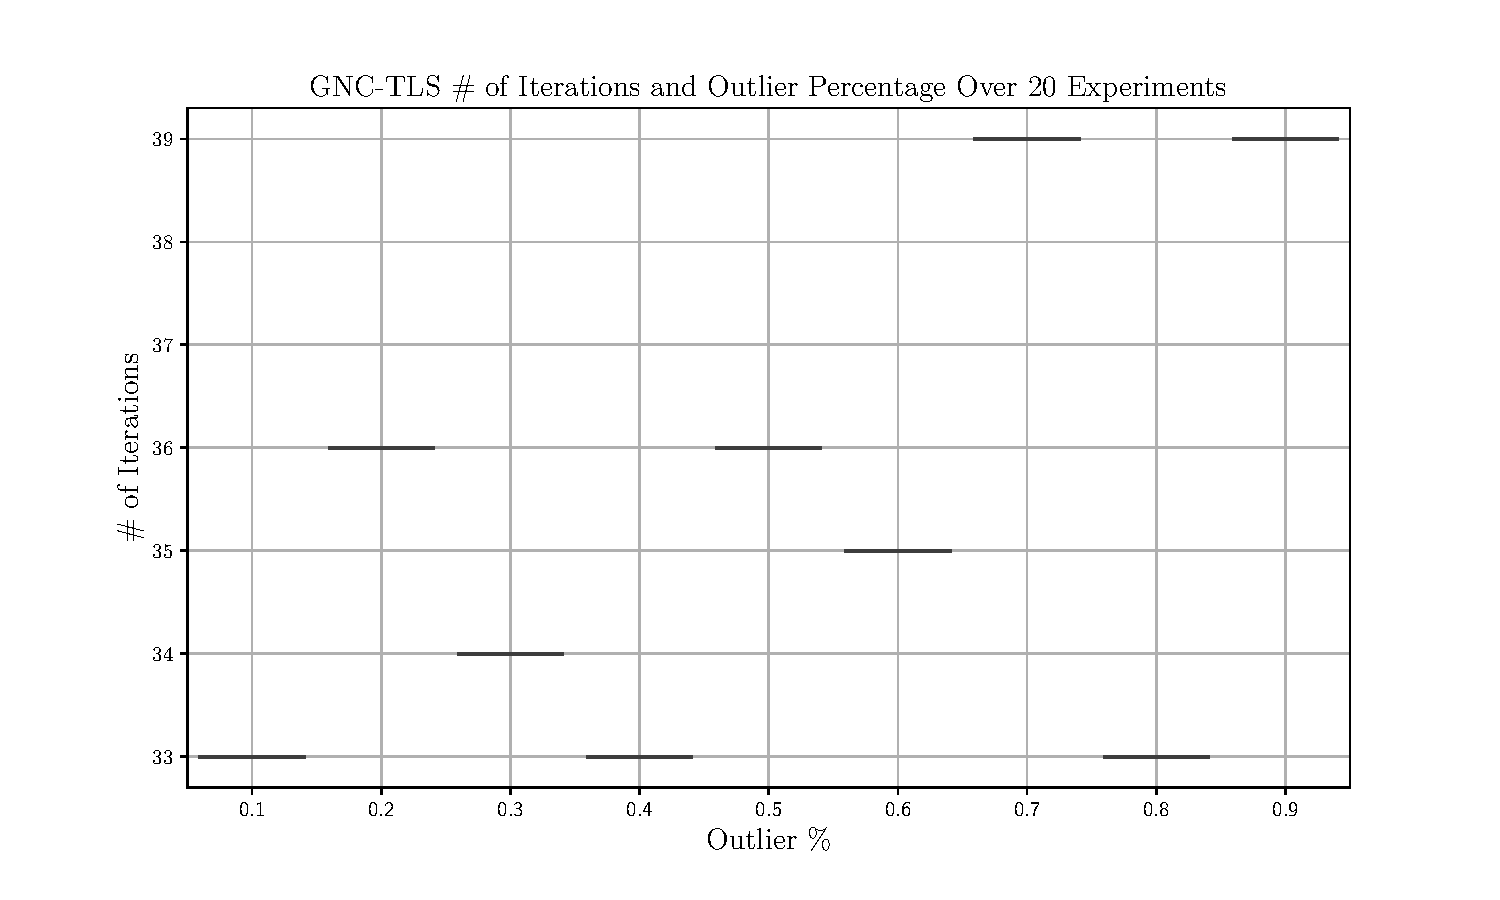
\includegraphics[width=\textwidth]{chapters/2-pose-estimation/fig/GNC-TLS-iterations-e.pdf}
% 		\caption{The source \gls{pc} generated from simulated contact points.\newline}
% 		\label{fig:pe-feature-filtered-pc2}
% 	\end{subfigure}
% 	% \hfill
% 	\begin{subfigure}[b]{0.48\textwidth}
% 		\centering
% 		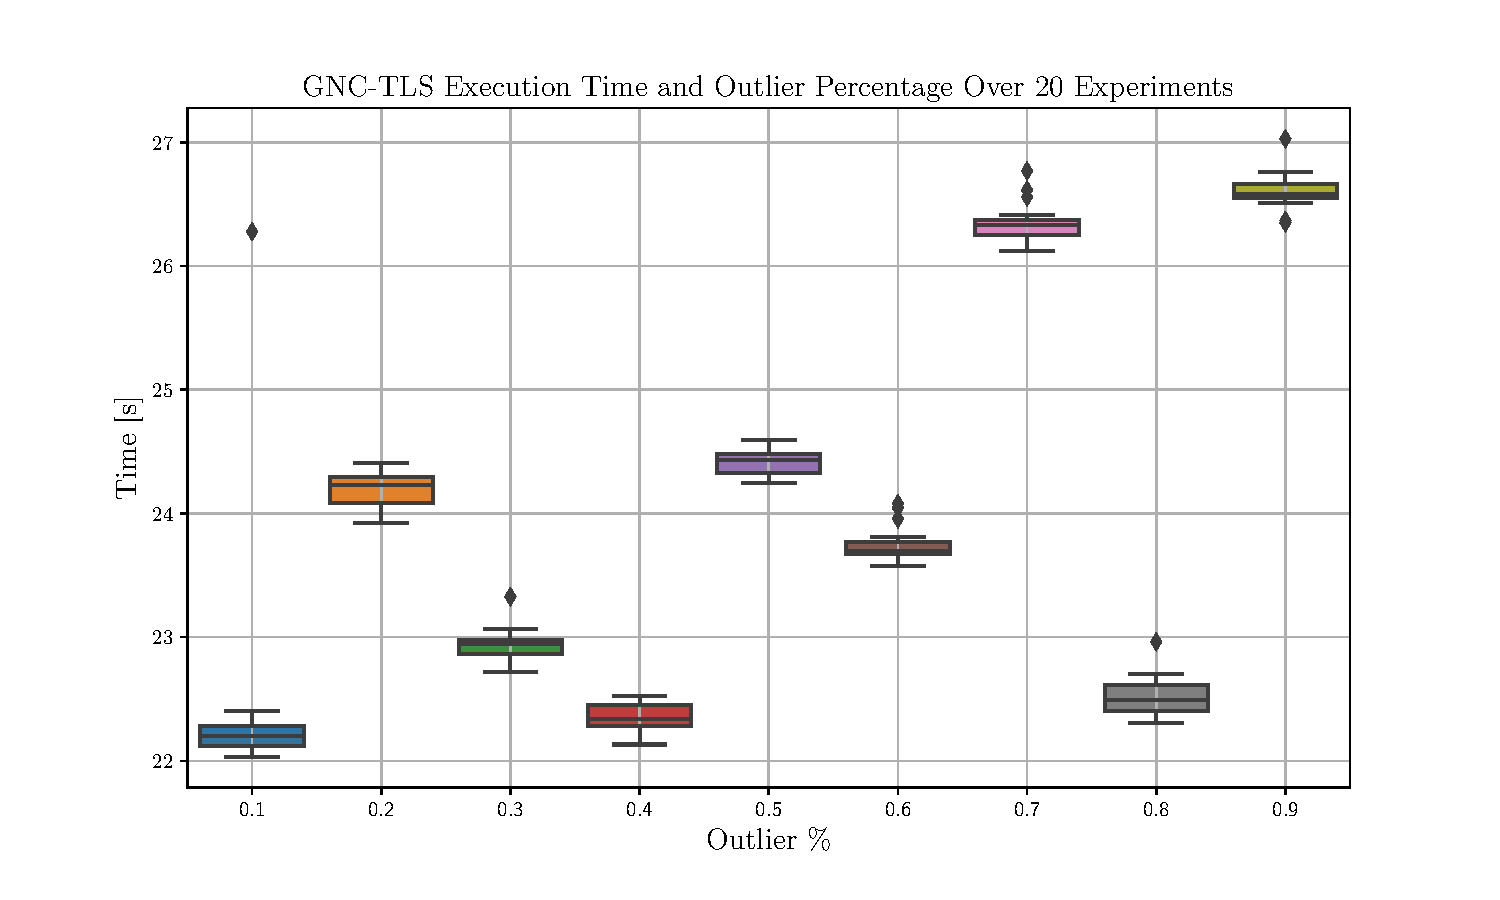
\includegraphics[width=\textwidth]{chapters/2-pose-estimation/fig/GNC-TLS-time-e.pdf}
% 		\caption{The target \gls{pc} generated by sampling the model mesh with \num{10,000} points.}
% 		\label{fig:pe-feature-unfiltered-pc2}
% 	\end{subfigure}
% 	\caption{3D plots showing the sampled source and target \gls{pc}s along with a plot showing both of them overlaid.}
% 	\label{fig:pe-filture-and-unfiltered-pc2}
% \end{figure}
\begin{figure}[!h]
	\begin{center}
		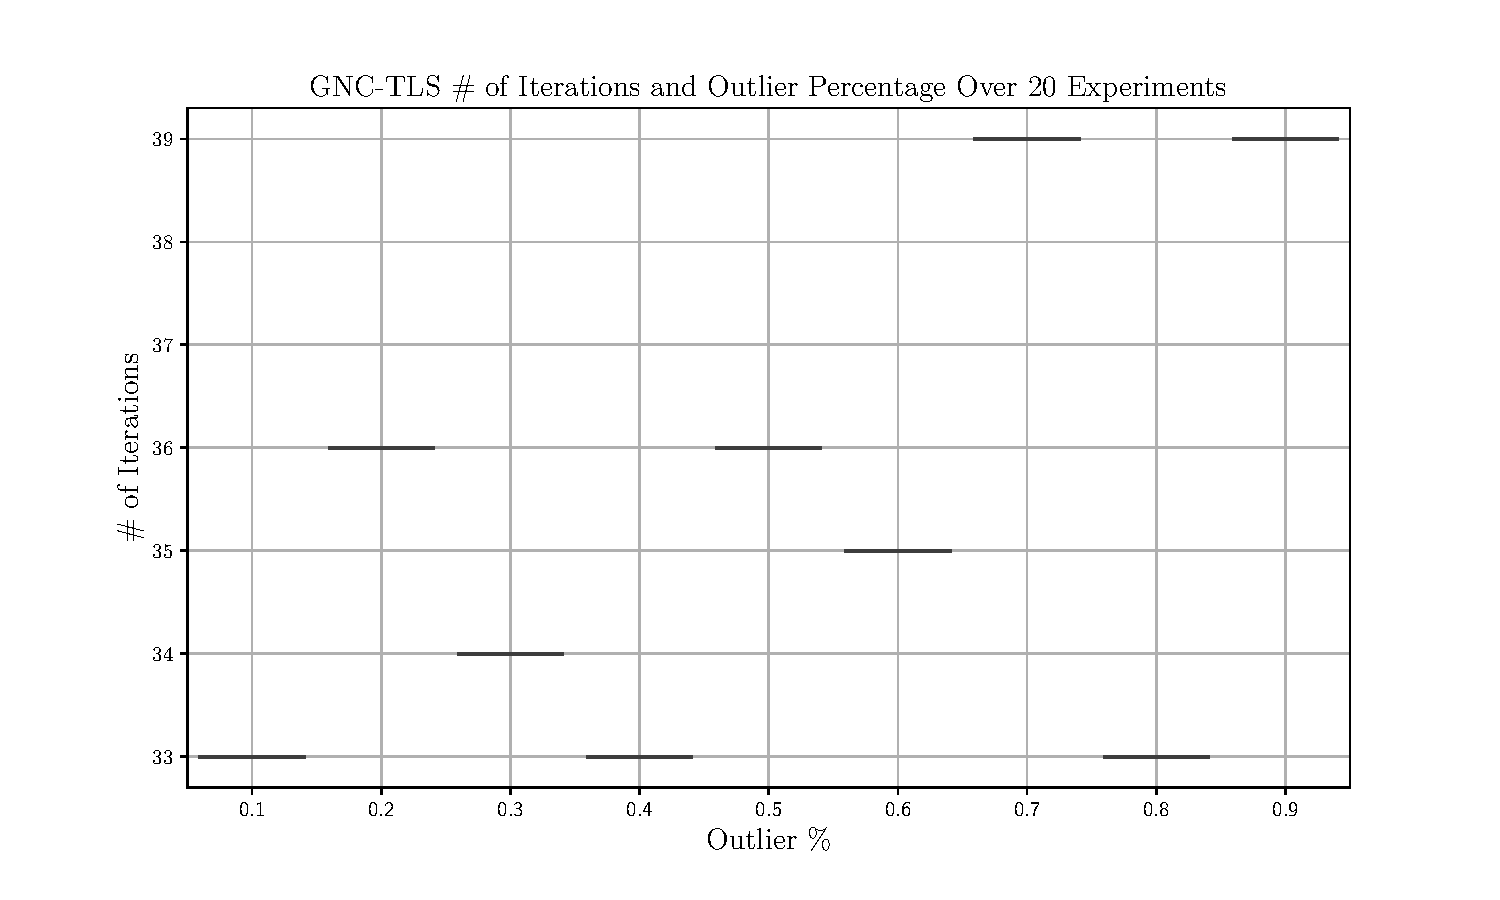
\includegraphics[width=\textwidth]{chapters/2-pose-estimation/fig/GNC-TLS-iterations-e.pdf}
	\end{center}
	\caption{Cost function for the \gls{tls} with }
	\label{fig:GNC-TLS-iterations-e}
\end{figure}

\begin{figure}[!h]
	\begin{center}
		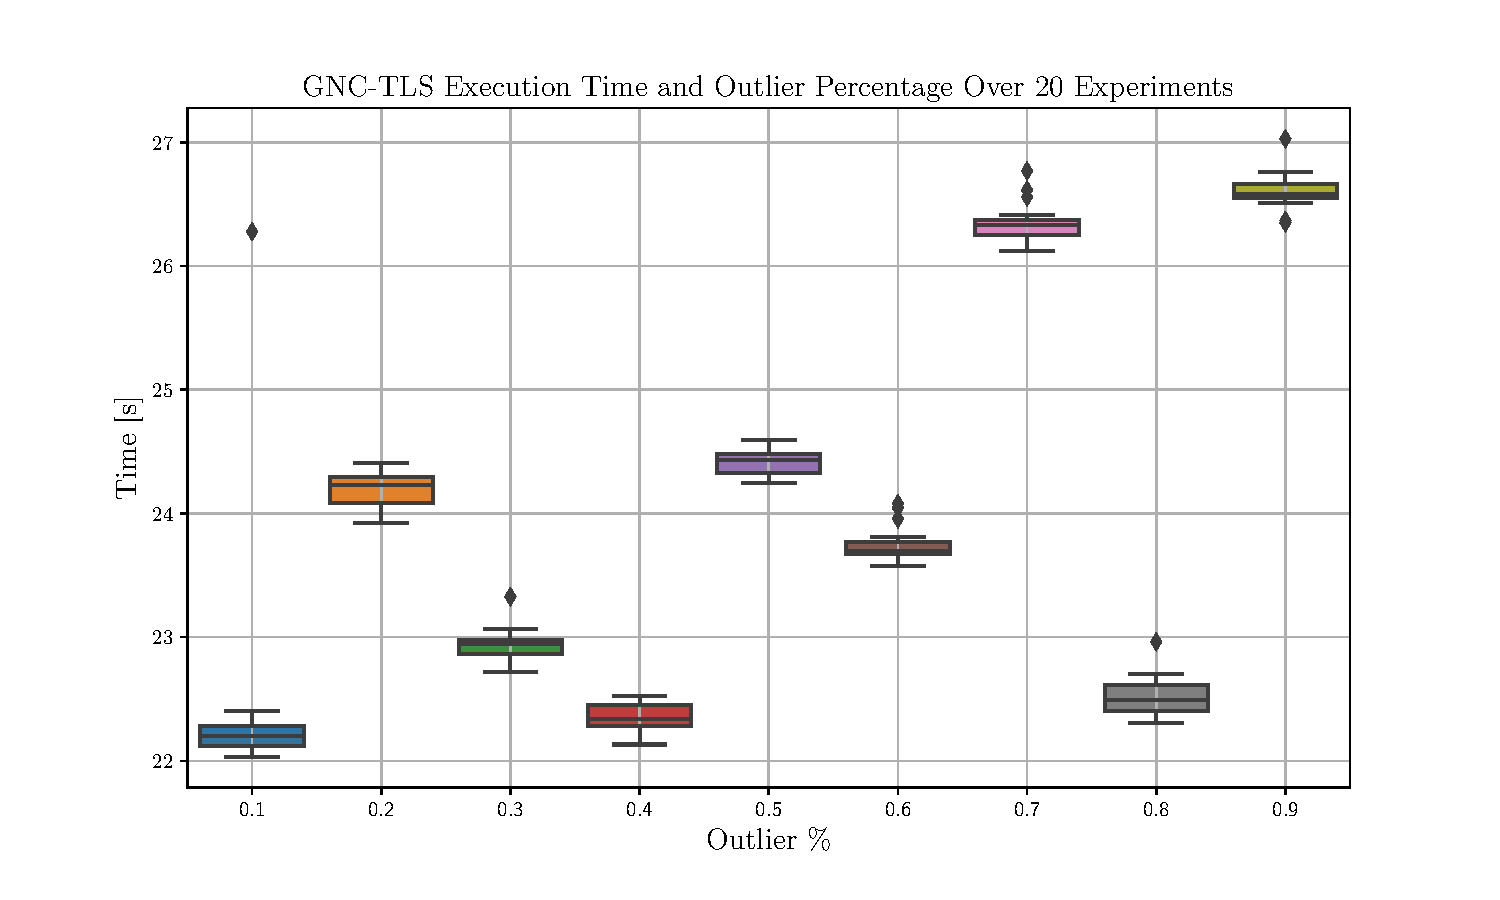
\includegraphics[width=\textwidth]{chapters/2-pose-estimation/fig/GNC-TLS-time-e.pdf}
	\end{center}
	\caption{Cost function for the \gls{tls} with }
	\label{fig:GNC-TLS-time-e}
\end{figure}

\begin{figure}[!h]
	\begin{center}
		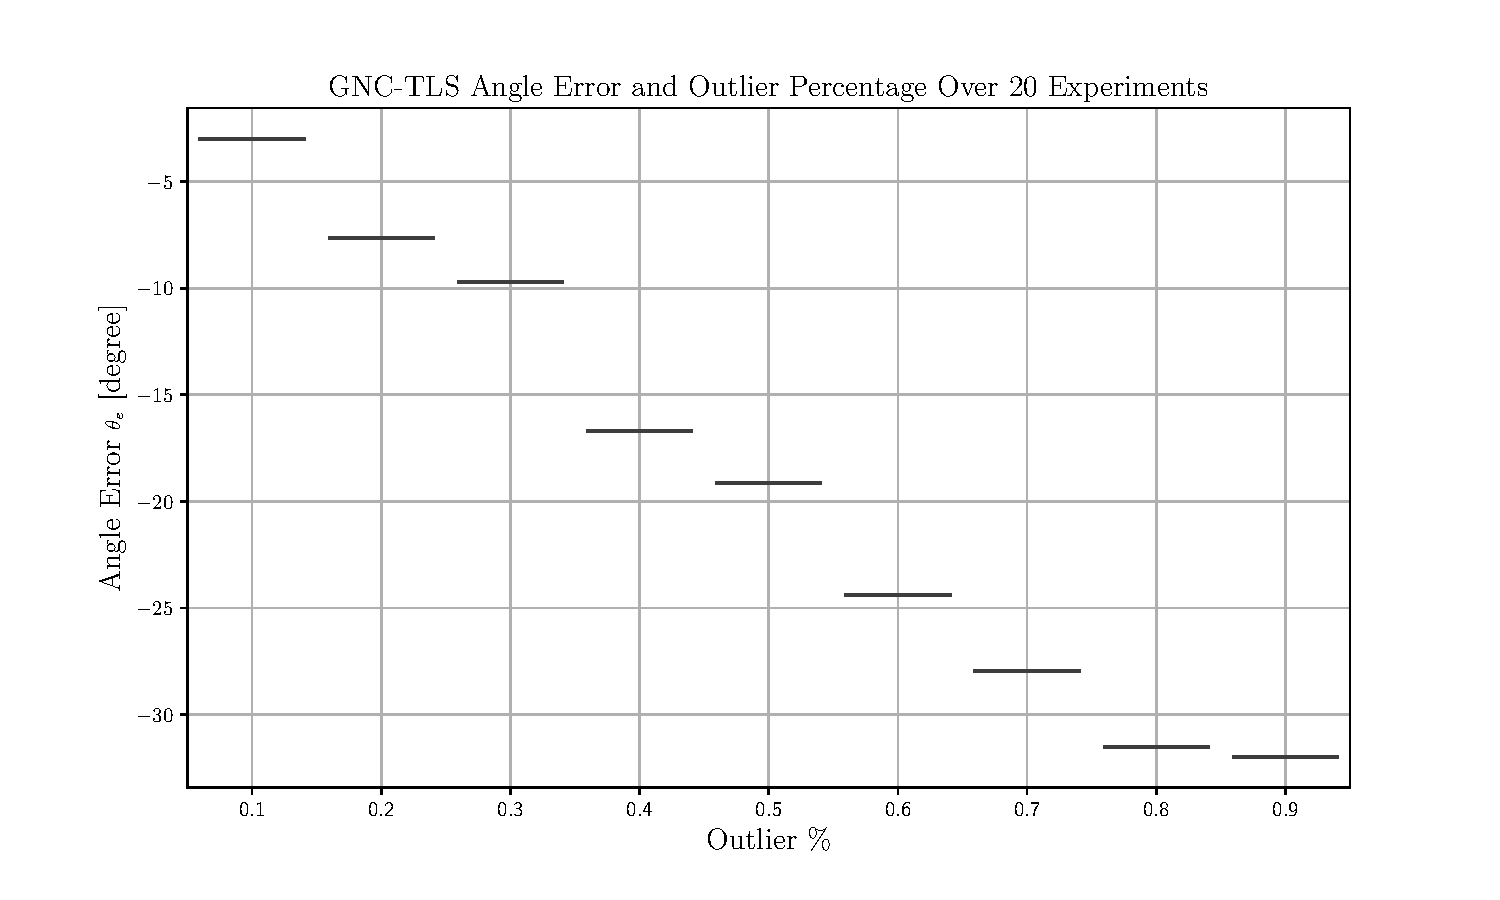
\includegraphics[width=\textwidth]{chapters/2-pose-estimation/fig/GNC-TLS-theta-e.pdf}
	\end{center}
	\caption{Cost function for the \gls{tls} with }
	\label{fig:GNC-TLS-theta-e}
\end{figure}

\begin{figure}[!h]
	\begin{center}
		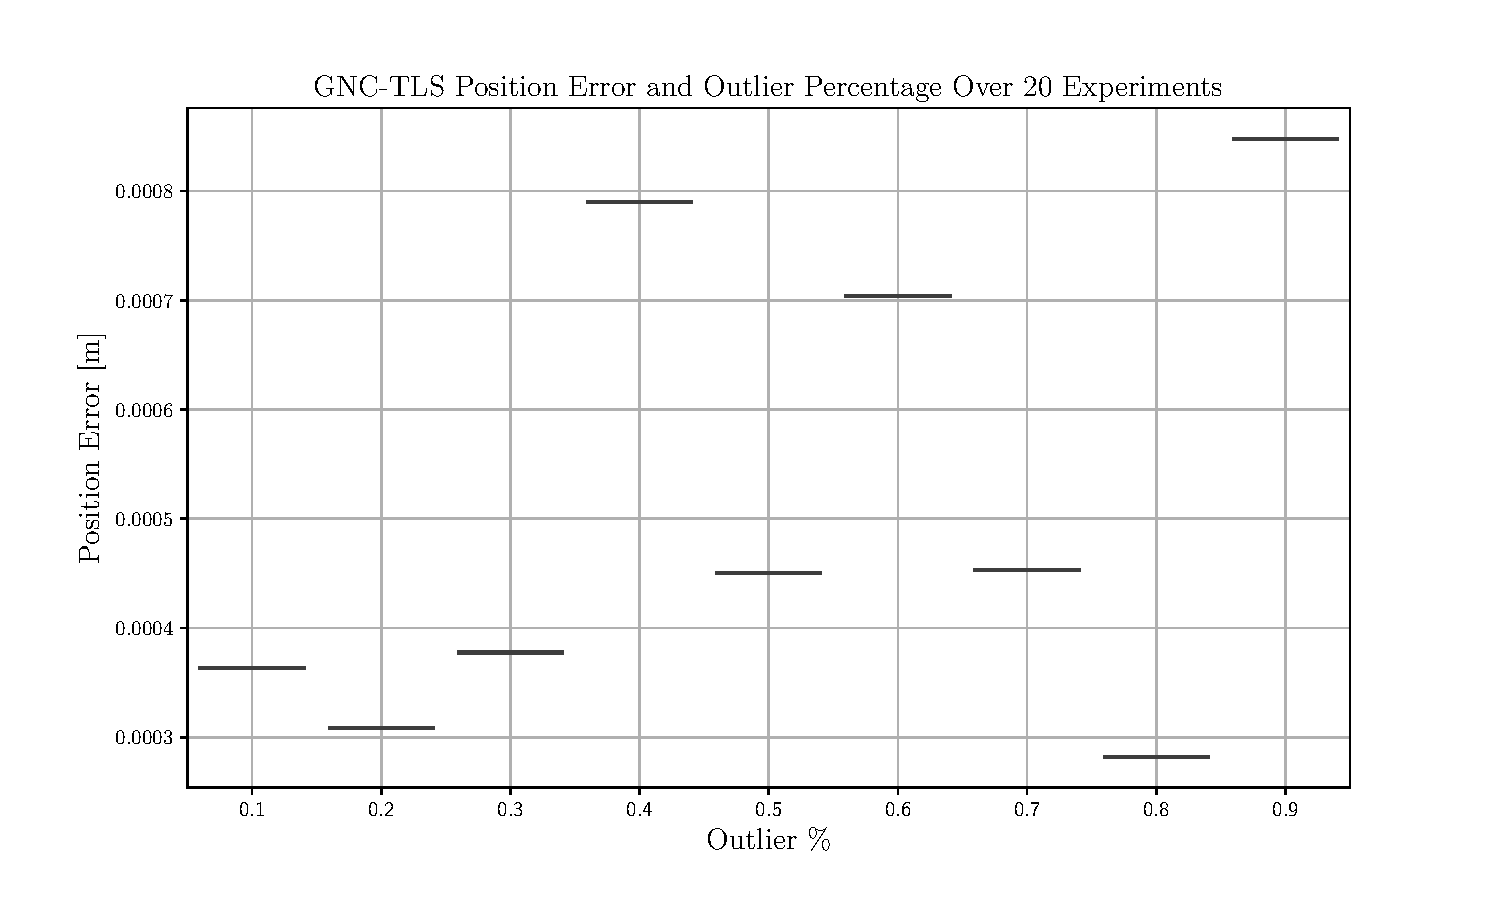
\includegraphics[width=\textwidth]{chapters/2-pose-estimation/fig/GNC-TLS-t-e.pdf}
	\end{center}
	\caption{Cost function for the \gls{tls} with }
	\label{fig:GNC-TLS-t-e}
\end{figure}

\newpage
\subsection{Weight Convergence Data}\label{sec:weight-convergence-data}

In~\figref{fig:GNC-TLS-w-history-conv} the weight history is shown for a single run with \SI{10}{\percent} outliers, meaning how each weight entry changes value for each outer loop iteration. It can here be seen that the weight tends to converge either to \num{0} or \num{1} as one would come to expect.\medskip

\figref{fig:GNC-TLS-w-run-conv} show the number of non-zero entries for \num{20} experiments with \SI{10}{\percent} outliers.

\begin{figure}[!h]
	\begin{center}
		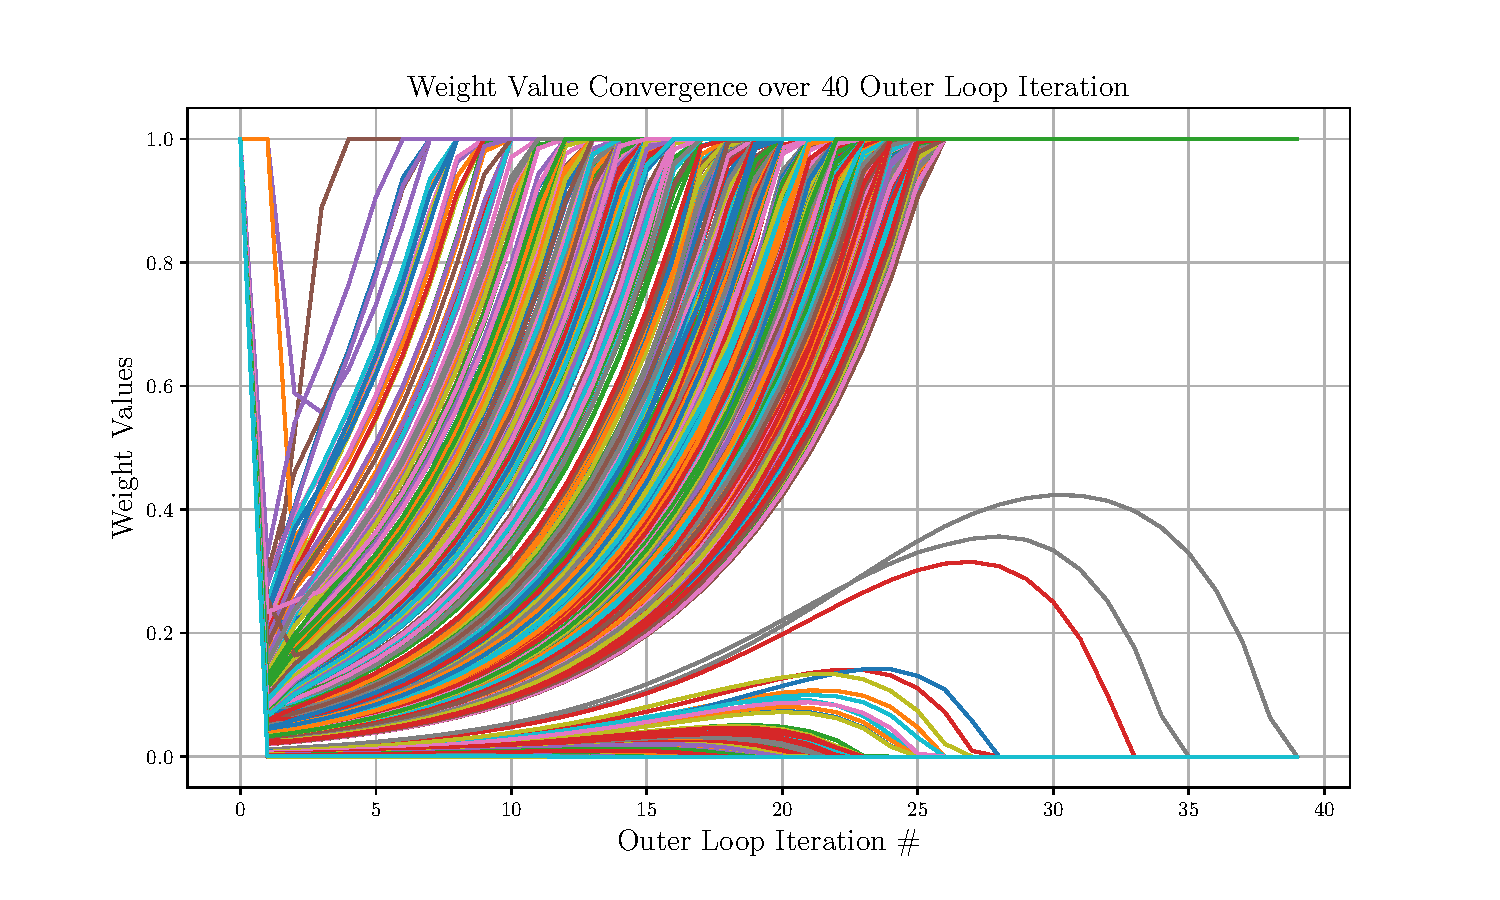
\includegraphics[width=\textwidth]{chapters/2-pose-estimation/fig/GNC-TLS-w-history-conv.pdf}
	\end{center}
	\caption{Cost function for the \gls{tls} with }
	\label{fig:GNC-TLS-w-history-conv}
\end{figure}

\begin{figure}[!h]
	\begin{center}
		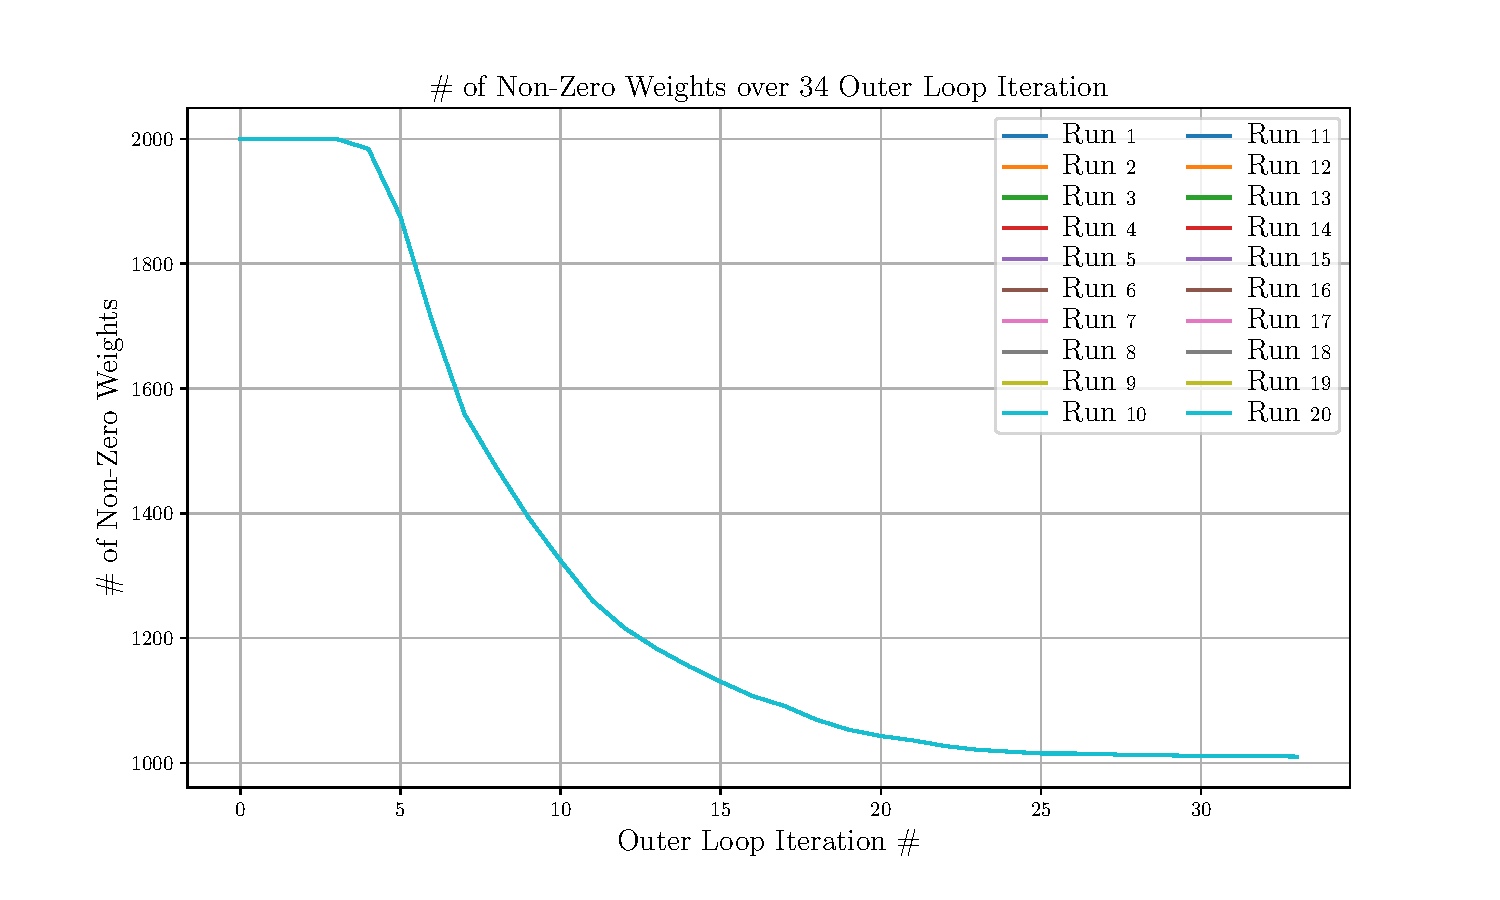
\includegraphics[width=\textwidth]{chapters/2-pose-estimation/fig/GNC-TLS-w-run-10-conv.pdf}
	\end{center}
	\caption{Cost function for the \gls{tls} with }
	\label{fig:GNC-TLS-w-run-conv}
\end{figure}


\section{Discussion \& Conclusion}\label{sec:2-pose-estimation-discussion}

% The results found showed the legitimacy of the \gls{gnc}+\gls{rcqp} method for pose estimation in the case of synthetic data. The methods could not be applied successfully to the sampled data due to lacking features.

% the problems include that it was not possible to find a functional number of feature correspondences. This is suggested based on the sparsity of the point cloud and techniques for intelligent probing is necessary.

% It was possible in the synthetic case, to successfully solve the pose estimation problem satisfactory for outlier percentage of \SI{10}{\percent} regarding the orientation estimation, while the position estimation performed satisfactorily. At \SI{20}{\percent} outliers the angle error reaches \SI{-7.66}{\degree} and thus does not fulfill the success criteria, which holds for greater outlier ratios as well. 

% The weight convergence results show an expected convergence towards \num{0} and \num{1}, yet the values at which the weight converges are yet to be explained. The expected result would here be that the number of non-zero weights should converge to \num{900} for a \SI{10}{\percent} outlier case. The remaining graphs can be seen in~\appref{app:pose-estimation-weight-convergence}.


The obtained results demonstrate the effectiveness of the \gls{gnc}+\gls{rcqp} method for pose estimation when applied to synthetic data. However, when dealing with sampled data, the methods faced challenges due to the lack of discernible features. One of the main difficulties encountered was the inability to identify a sufficient number of feature correspondences. This limitation can be attributed to the sparsity of the point cloud, indicating the need for intelligent probing techniques to enhance feature detection. \medskip

In the case of synthetic data, the pose estimation problem was successfully solved with satisfactory results for orientation estimation, even in the presence of a \SI{10}{\percent} outlier percentage. However, as the outlier percentage increased to \SI{20}{\percent}, the angle error reached \SI{-7.66}{\degree}, failing to meet the desired success criteria. This trend persisted for higher outlier ratios as well. \medskip

The weight convergence analysis revealed an expected trend of convergence towards 0 and 1. However, the specific values at which the weights converged require further investigation and explanation. For example, in the case of a \SI{10}{\percent} outlier scenario, the expected outcome would be the convergence of the number of non-zero weights to \num{900}. Detailed graphs illustrating the weight convergence results can be found in~\appref{app:pose-estimation-weight-convergence}.\medskip

In summary, the \gls{gnc}+\gls{rcqp} method exhibited promising performance in pose estimation for synthetic data. However, challenges arose when working with sampled data, emphasizing the need for improved feature detection techniques. The angle error increased with higher outlier percentages, suggesting the importance of robustness in handling outliers. Further analysis is required to understand the convergence values of the weights and refine the pose estimation algorithm accordingly.

\pagebreak
\chapter{In-Hand Manipulation} \label{ch:3-in-hand-manipulation}

\section{Introduction} \label{sec:3-in-hand-manipulation-introduction}
Here we write the introduction for problem 3.


\section{Related Work} \label{sec:3-in-hand-manipulation-related-work}

Here we cite the related work by \texttt{\textbackslash cite\{source-label\}} like this \cite{recent-progress-in-technologies-for-tactile-sensors}




For history see hand book of robotics chapter 38, the first section.


\pagebreak
\chapter{System Integration} \label{ch:4-system-integration}

\section{Introduction} \label{sec:4-system-integration-introduction}
Here we write the introduction for the system integration.


% Here we cite the related work by \texttt{\textbackslash cite\{source-label\}} like this \cite{recent-progress-in-technologies-for-tactile-sensors}

\pagebreak
\chapter{Discussion} \label{ch:discussion}

\pagebreak
\chapter{Conclusion}\label{ch:conclusion}

this is the conclusion

% bibliography
\pagebreak
% \printbibliography[heading=bibintoc]
% \begin{multicols}{2}[\printbibheading]
% \printbibliography[heading=none]
% \end{multicols}
\printbibliography

\appendix
\chapter{Shadow Dexterous Hand - Technical Specifications}\label{app:shadow-dexterous-hand-technical-specifications}

\tabref{app:range-of-motion-shadow-hand} shows the \gls{rom} for the Shadow Dexterous Hand and \tabref{app:range-of-motion-human-hand} shown the \gls{rom} for a human hand. The shorthand abbreviations used in these tables can be seen listed in \tabref{app:joint-abbreviations}. The joints are numbered from fingertip to base and thus FF1 refers to the first joint after the fingertip on the first finger i.e. the index finger.
\begin{table}[!h]
\begin{center}
	\begin{tabular}{ |p{0.22\textwidth}|p{0.08\textwidth}|p{0.08\textwidth}|p{0.08\textwidth}|p{0.08\textwidth}|p{0.3\textwidth}| } 
	\hline
	\multicolumn{6}{|c|}{\textbf{\gls{rom} - Shadow Dexterous Hand}} \\ \hline
	\textbf{Joint(s)} & \textbf{Min deg} & \textbf{Max deg} & \textbf{Min rad} & \textbf{Max rad} & \textbf{Notes} \\ \hline
	FF1, MF1, RF1, LF1 &0&90&0&1.571  & \multirow{2}{4em}{Coupled}\\ \cline{1-5}
	FF2, MF2, RF2, LF2 & 0   & 90 & 0      & 1.571 & \\ \hline
	FF3, MF3, RF3, LF3 & -15 & 90 & -0.262 & 1.571 & \\ \hline
	FF4, MF4, RF4, LF4 & -20 & 20 & -0.349 & 0.349 & \\ \hline
	LF5&0&45&0&0.785 &  \\ \hline
	TH1&-15&90&-0.262&1.571 &  \\ \hline
	TH2&-40&40&-0.698&0.698 &  \\ \hline
	TH3&-12&12&-0.209&0.209 &  \\ \hline
	TH4&0&70&0&1.222& \\ \hline
	TH5&-60&60&-1.047&1.047& \\ \hline
	WR1&-40&28&-0.698&0.489& \\ \hline
	WR2&-28&10&-0.489&0.174& \\ \hline
	\end{tabular}
	\caption{The ranges of motion for each joint in the Shadow Dexterous Hand~\cite{range-of-motion-shadow-hand}.}
	\label{app:range-of-motion-shadow-hand}
\end{center}
\end{table}

\begin{table}[!h]
	\begin{center}
		\begin{tabular}{ |p{0.22\textwidth}|p{0.08\textwidth}|p{0.08\textwidth}|p{0.08\textwidth}|p{0.08\textwidth}|p{0.3\textwidth}| } 
		\hline
		\multicolumn{6}{|c|}{\textbf{\gls{rom} - Human Hand}} \\ \hline
		\textbf{Joint(s)} & \textbf{Min deg} & \textbf{Max deg} & \textbf{Min rad} & \textbf{Max rad} & \textbf{Latin Name} \\ \hline
		TH1 & -15 & 80 & & & Interphalangeal (IP) \\ \hline
		TH2 + TH3 & -10 & 55 & & & Metacarpophalangeal (MCP)\\ \hline
		TH4 +TH5  & -10 & 55 & & & Carpometacarpal (CMC)\\ \hline
		FF1, MF1, RF1, LF1 & 0 & 80 & & & Distal interphalangeal (DIP) \\ \hline
		FF2, MF2, RF2, LF2 & 0 & 100 & & & Proximal interphalangeal (PIP) \\ \hline
		FF3, MF3, RF3, LF3 & -45 & 90 & & & Metacarpophalangeal (MCP) \\ \hline
		WR1 &-80&80& & & Radiocarpal \\ \hline
		WR2 &-28&20& & & Radiocarpal \\ \hline
		\end{tabular}
		\caption{The theoretical \gls{rom} for each finger joint in human hand~\cite{continuous-and-simultaneous-estimation-of-finger-kinematics-using-inputs-from-an-emg-to-muscle-activation-model} and found \gls{rom} for the wrist joints~\cite{functional-wrist-motion:-a-biomechanical-study}.}
		\label{app:range-of-motion-human-hand}
	\end{center}
\end{table}

\begin{table}[!h]
	\begin{center}
		\begin{tabular}{ |l|l| } 
		\hline
		\multicolumn{2}{|c|}{\textbf{Joint Name Abbreviation}} \\ \hline
		\textbf{Abbreviation} & \textbf{Full Name} \\ \hline
		FF & First Finger \\ \hline 
		MF & Middle Finger \\ \hline 
		RF & Ring Finger \\ \hline 
		LF & Little Finger \\ \hline 
		WR & Wrist \\ \hline 
		\end{tabular}
		\caption{The abbreviations used to reference ~\cite{joint-abbreviations-shadow-hand}.}
		\label{app:joint-abbreviations}
	\end{center}
	\end{table}

To compare the kinematic structure of the Shadow Dexterous Hand and a human hand, see~\figref{app:human-and-robot-hand-kinematics}.

\begin{figure}[!h]
	\centering
	\begin{subfigure}[b]{0.3\textwidth}
		\centering
		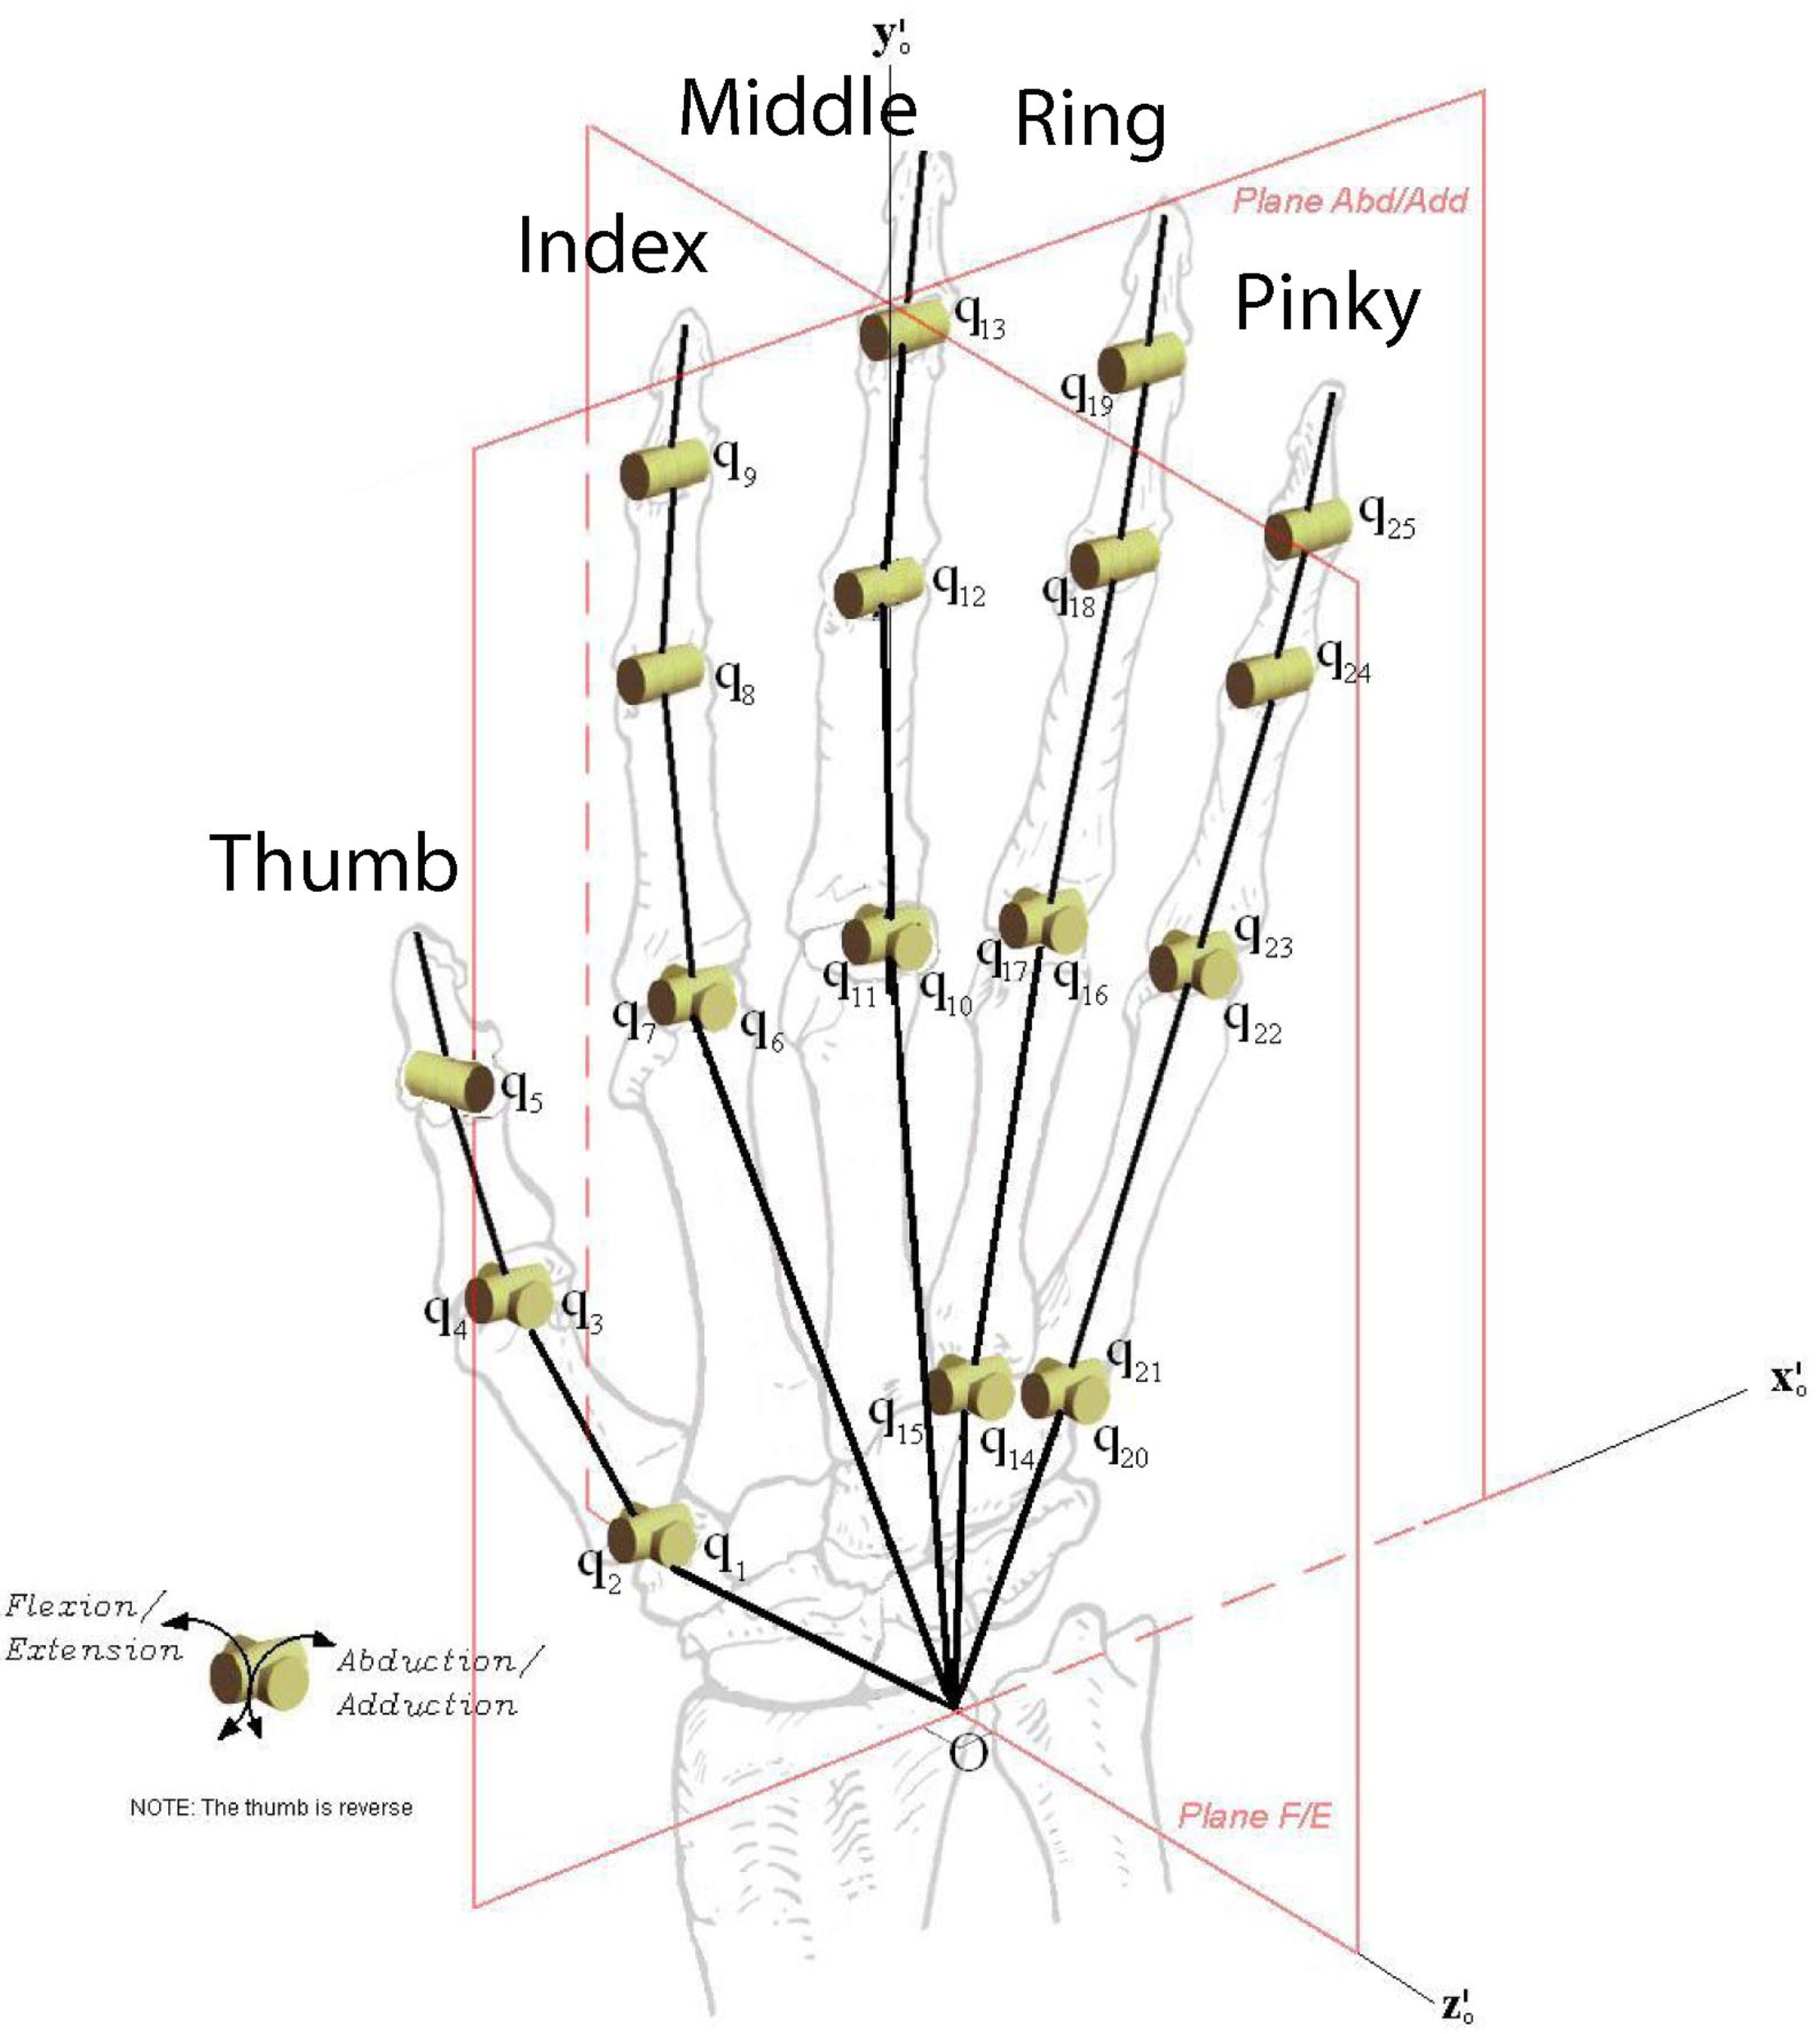
\includegraphics[width=\textwidth]{chapters/appendix/fig/human-hand-kinematics.pdf}
		\caption{The kinematic tree of a human hand according to~\cite{grasp-synthesis-algorithms-for-multifingered-robot-hands}.}
		\label{app:human-hand-kinematics}
	\end{subfigure}
	\hfill
	\begin{subfigure}[b]{0.69\textwidth}
		\centering
		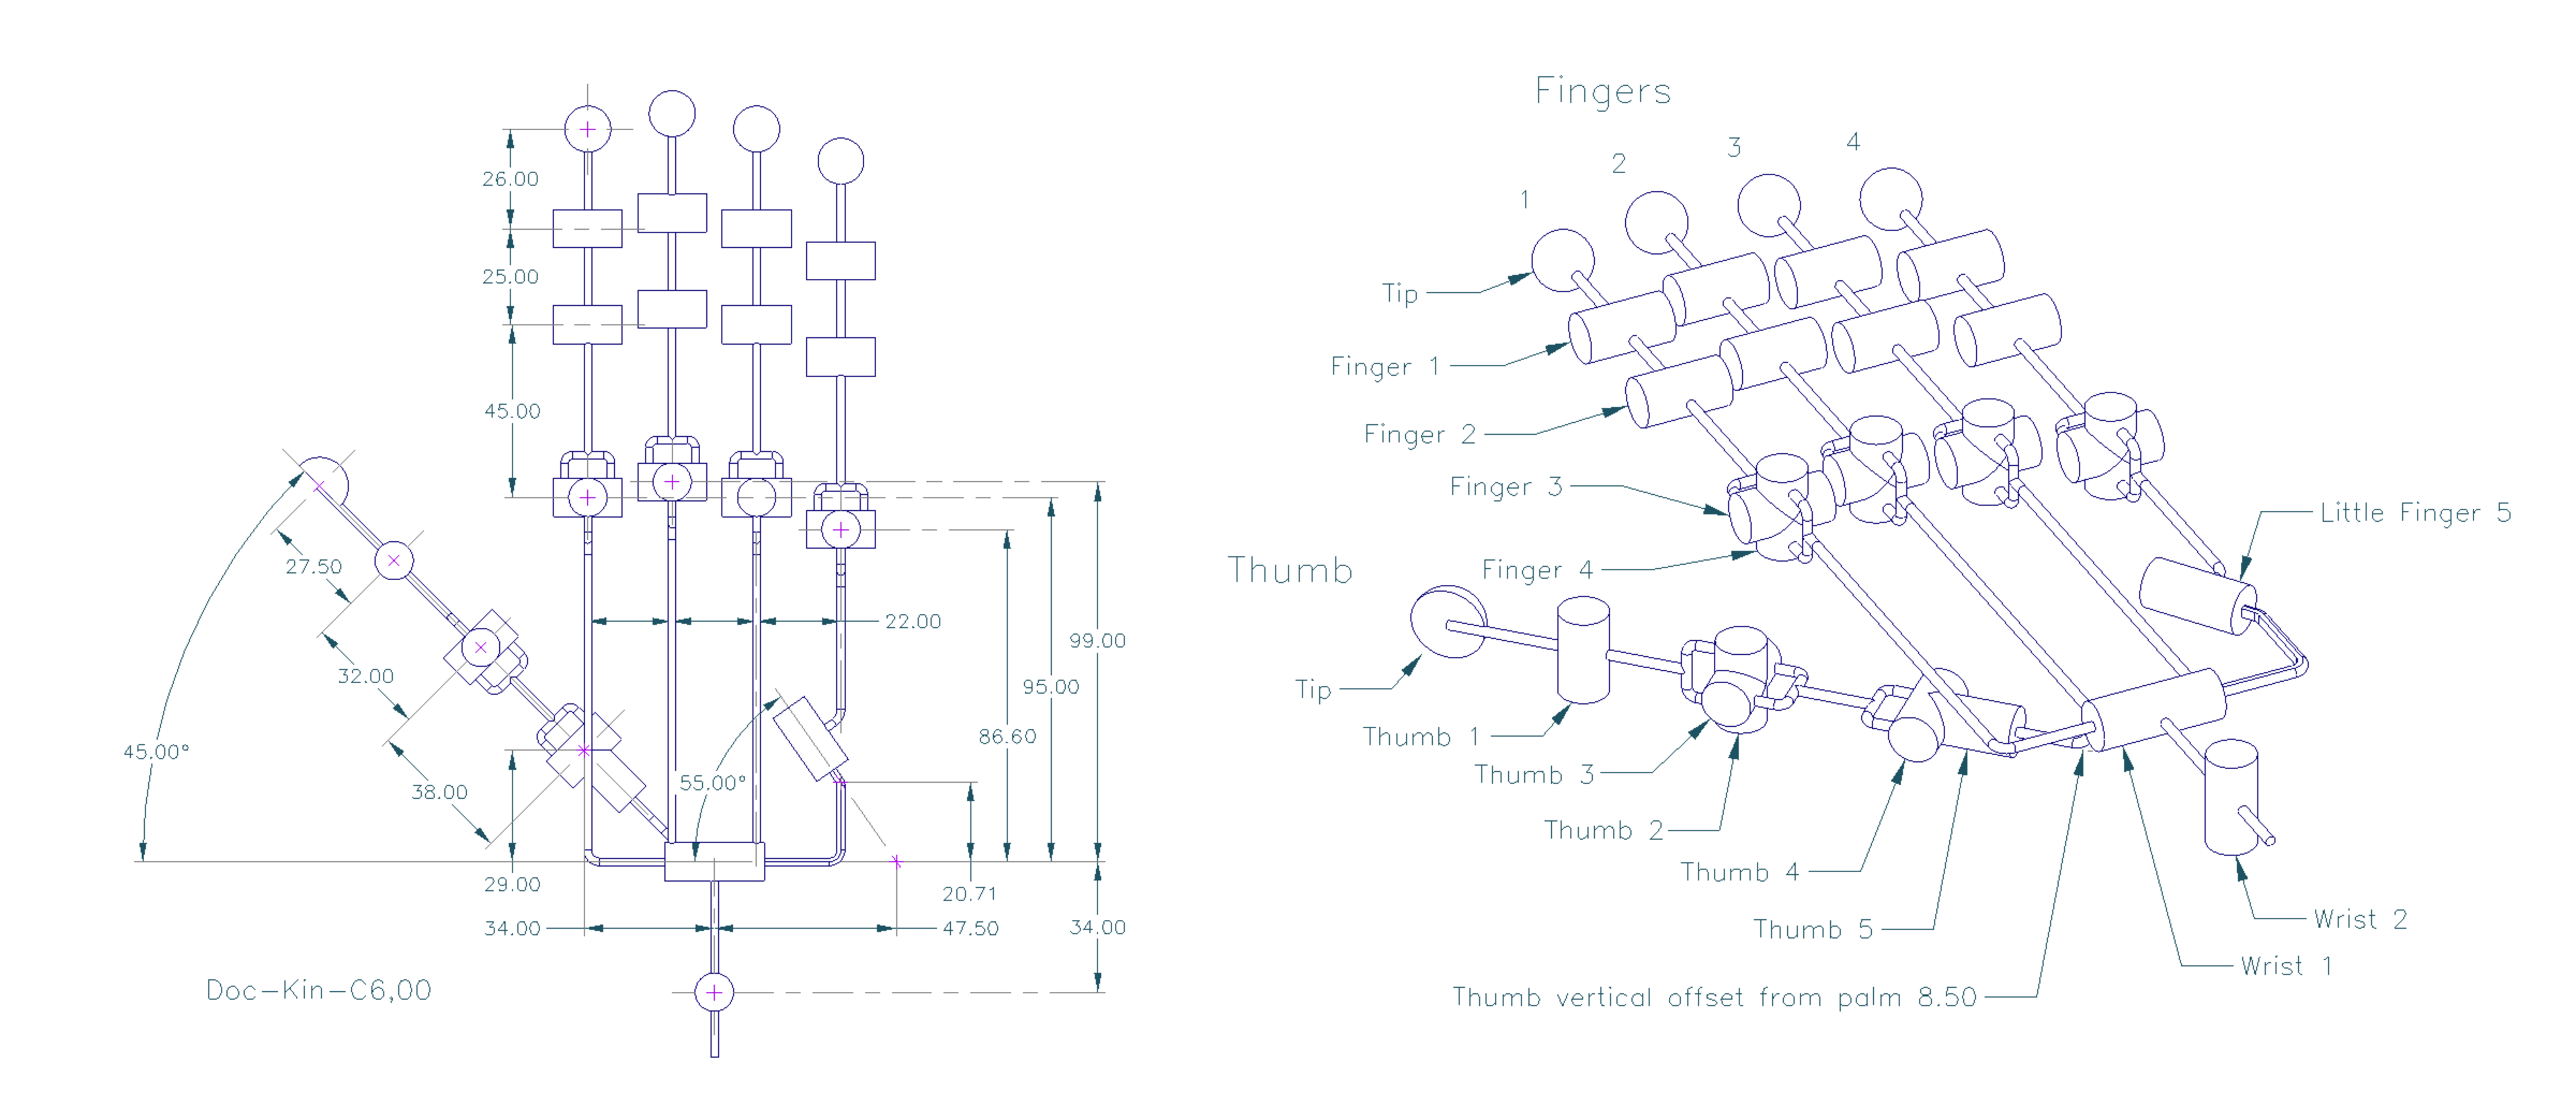
\includegraphics[width=\textwidth]{chapters/appendix/fig/robot-hand-kinematics.pdf}
		\caption{The kinematic tree of the Shadow Dexterous Hand according to~\cite{robot-hand-kinematics}. \newline}
		\label{app:robot-hand-kinematics}
	\end{subfigure}
	\caption{The kinematic trees of a human hand and the Shadow Dexterous hand.}
	\label{app:human-and-robot-hand-kinematics}
\end{figure}

\chapter{Tactile Perception - Simulated Electrode Activations}\label{app:tactile-perception-simulated-electrode-activations}

Below three 

\begin{figure}[!h]
	\begin{center}
		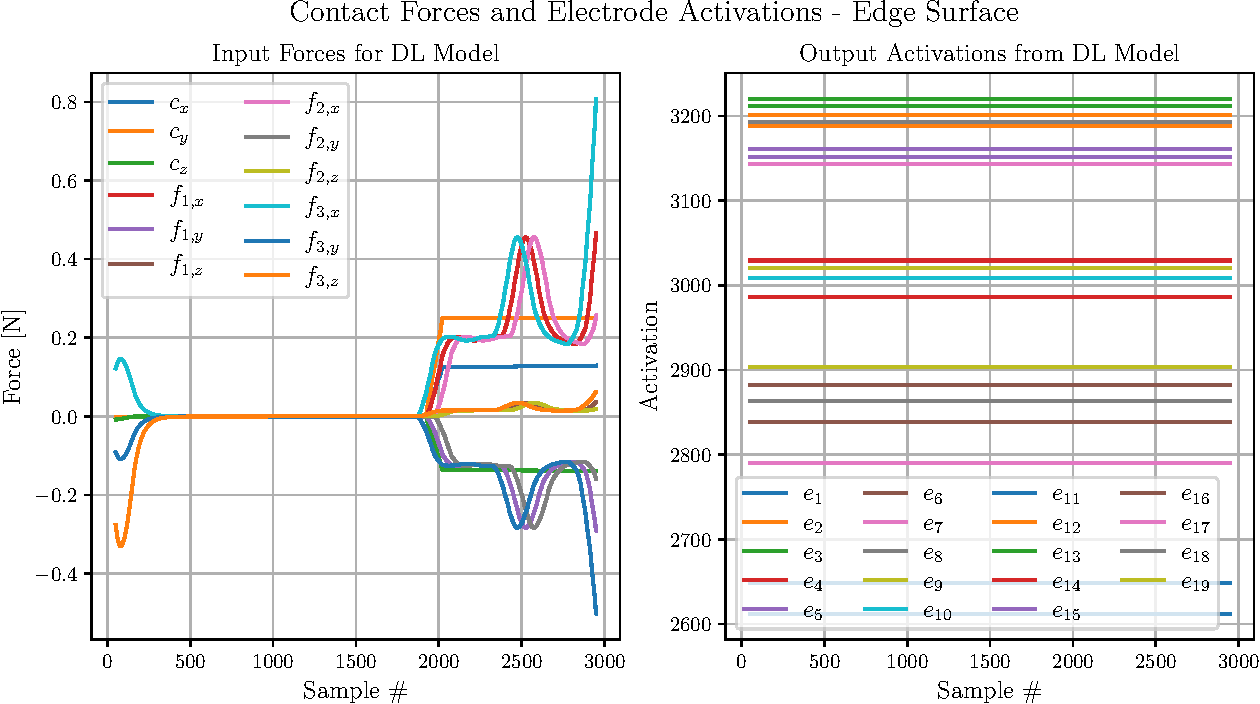
\includegraphics[width=\textwidth]{chapters/1-tactile-perception/fig/matplotlib/edge-contact-graph.pdf}
	\end{center}
	\caption{he simulated tactile electrode activations when the simulated Shadow Dexterous hand's index finger is in contact with an edge.}
	\label{app:edge-contact-graph}
\end{figure}

\begin{figure}[!h]
	\begin{center}
		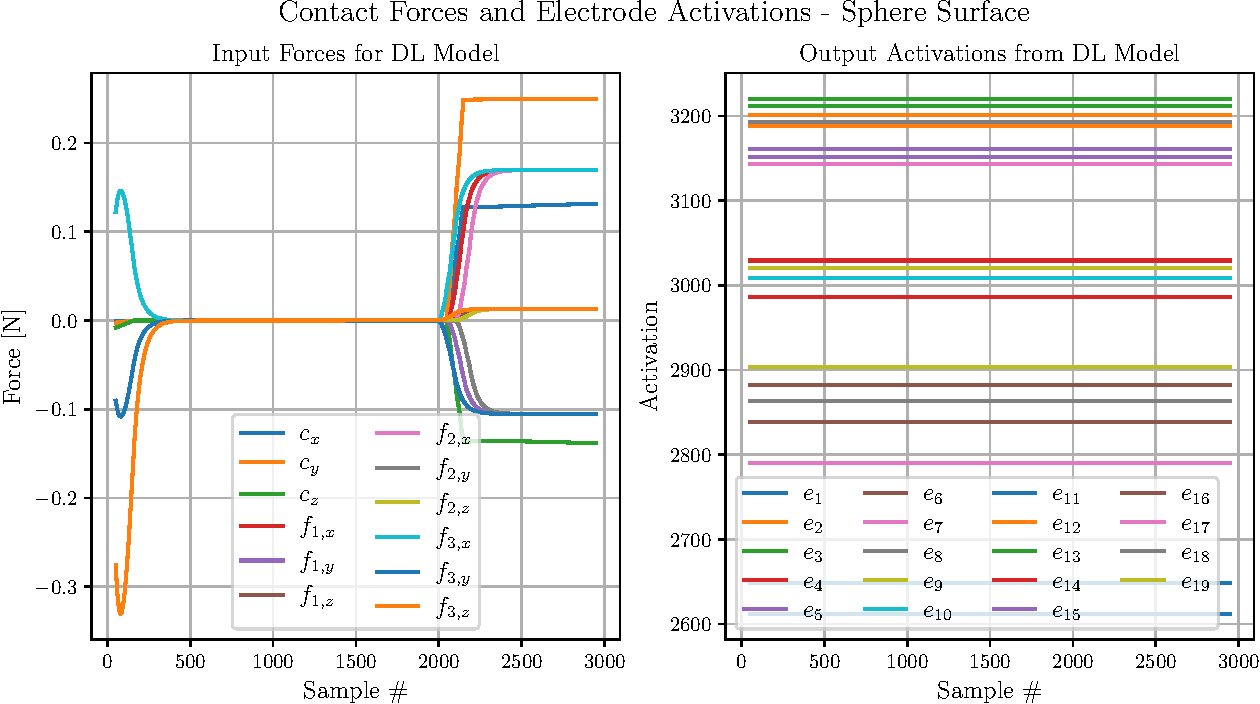
\includegraphics[width=\textwidth]{chapters/1-tactile-perception/fig/matplotlib/sphere-contact-graph.pdf}
	\end{center}
	\caption{The simulated tactile electrode activations when the simulated Shadow Dexterous hand's index finger is in contact with a smooth surface.}
	\label{app:smooth-contact-graph}
\end{figure}

\begin{figure}[!h]
	\begin{center}
		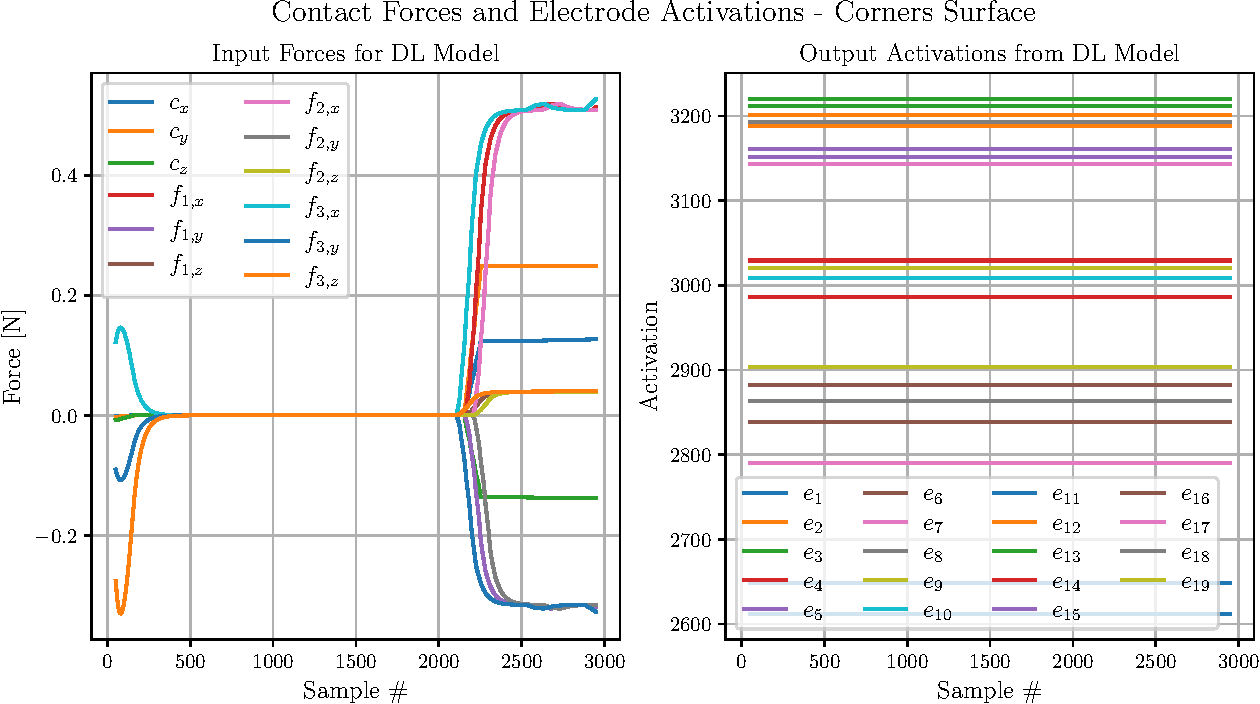
\includegraphics[width=\textwidth]{chapters/1-tactile-perception/fig/matplotlib/corners-contact-graph.pdf}
	\end{center}
	\caption{The simulated tactile electrode activations when the simulated Shadow Dexterous hand's index finger is in contact with a corner.}
	\label{app:corner-contact-graph}
\end{figure}

\end{document}